%% LyX 2.1.4 created this file.  For more info, see http://www.lyx.org/.
%% Do not edit unless you really know what you are doing.
\documentclass[a4paper,ngerman,naustrian,DIV=12,BCOR=1cm]{scrbook}
\usepackage[T1]{fontenc}
\usepackage[utf8]{inputenc}
\usepackage{fancyhdr}
\pagestyle{fancy}
\setcounter{secnumdepth}{3}
\usepackage{babel}
\usepackage{textcomp}
\usepackage{url}
\usepackage{makeidx}
\makeindex
\usepackage{graphicx}
\PassOptionsToPackage{normalem}{ulem}
\usepackage{ulem}
\usepackage[unicode=true,
 bookmarks=true,bookmarksnumbered=false,bookmarksopen=false,
 breaklinks=true,pdfborder={0 0 0},backref=false,colorlinks=false]
 {hyperref}
\hypersetup{pdftitle={Diplomarbeit Titel},
 pdfauthor={Wer auch immer},
 pdfsubject={Diplomarbeit},
 pdfkeywords={dies, das}}

\makeatletter

%%%%%%%%%%%%%%%%%%%%%%%%%%%%%% LyX specific LaTeX commands.
\pdfpageheight\paperheight
\pdfpagewidth\paperwidth

%% Because html converters don't know tabularnewline
\providecommand{\tabularnewline}{\\}

%%%%%%%%%%%%%%%%%%%%%%%%%%%%%% Textclass specific LaTeX commands.
\newcommand{\strong}[1]{\textbf{#1}}
\newcommand{\code}[1]{\texttt{#1}}

%%%%%%%%%%%%%%%%%%%%%%%%%%%%%% User specified LaTeX commands.
%%%%%%%%%%%%
% Latex-Vorspann
\usepackage{lastpage}
\usepackage{listings}
\usepackage{blindtext}

%% geht nicht mit jeder Latex Variante, gibt aber ein schöneres Layout
\usepackage{microtype}

%% Aufzählungen nicht so weit einrücken
\usepackage{enumitem}
%\setitemize{leftmargin=*}

%\usepackage{caladea}
%\usepackage[T1]{fontenc}
\usepackage{lmodern}

\usepackage{xspace}

%% für pandoc
%% maximale Breite der Bilder
\usepackage{graphicx}
\setkeys{Gin}{width=0.90\linewidth,keepaspectratio}
\providecommand{\tightlist}{%
\setlength{\itemsep}{0pt}\setlength{\parskip}{0pt}}

%um Schusterjungen und Hurenkinder vermeiden zu können
\usepackage{needspace}

%Farbpaket
\usepackage{xcolor}

%Für Bilddarstellung
\usepackage{subfigure}
\usepackage{float}
%\usepackage{subcaption}

%Darstellung im Abbildungsverzeichnis
\usepackage[subfigure]{tocloft}
\settowidth{\cftfignumwidth}{14.26\quad}
\setlength{\cftfignumwidth}{12mm}


%Einheitendarstellung
\usepackage{siunitx}
\sisetup{
  locale = DE ,
  per-mode = symbol
}


\usepackage{longtable}

%%%%%%%%%%% GLOSSAR teil 1/2 - muss getestet werden
\usepackage[toc,acronym]{glossaries}
\makeglossaries
%%%%%%%%%%%%%%%%%%%%%%%%%%%%%%%% BEISPIEL

% im Dokument: alles mit \gls{xxx} kann man anklicken :3

\newglossaryentry{partnership}{
	name=Partnerschaft,
	plural=Partnerschaften,
	description={Um Dateien/Dateiblöcke extern speichern zu können, muss eine
	sogenannte Partnerschaft mit anderen Geräten eingangen werden, bei der man
	Dateiblöcke auf den jeweilig anderen Geräten speichert, während man selber
	Speicherplatz für diese Partner freigibt, in dem deren verschlüsselte
	Dateiblöcke	gespeichert werden}
}

\newglossaryentry{syncpartner}{
	name=Synchronisationspartner,
	plural=Synchronisationspartner,
	description={Gerät mit dem der \sblit-Ordner synchronisiert wird}
}

\newglossaryentry{filecloud}{
	name=Filecloud,
	description={Externer Speicher im Internet, auf dem Dateien gespeichert werden
	können. Meistens bestehend aus einem oder mehreren Servern}
}

%%%%%% Glossar mit Akronym


%\newglossaryentry{gls_aes}{
%	name=Advanced Encryption Standard,
%	description={Standard-Verschlüsselungsverfahren für \glspl{link}},
%	see={[Siehe:]{link}}
%}
%\newacronym[see={[Glossar:]{gls_aes}}]{aes}{AES}{Advanced Encryption Standard\glsadd{gls_aes}}

%\newglossaryentry{gls_gcm}{
%	name=Galois/Counter Mode,
%	description={Standard-Betriebsmodus für die Verschlüsselung von \glspl{link} mit \acrshort{aes}}, %%%% glspl: Link zu Thema "Link" :b (bloedes bsp)
%}
%\newacronym[see={[Glossar:]{gls_gcm}}]{gcm}{GCM}{Galois/Counter Mode\glsadd{gls_gcm}}

%%%%%%%%%%%%%% Unsere Glossareinträge (evtl mit Akronym)

\newglossaryentry{Mitglied}{
	name=Mitglied,
  plural=Mitglieder,
	description={Mitglieder (eng. members) sind Variablen in einer Struktur}
}


%%% im dokument \glslink{Struktur}{Strukturen} muss getestet werden

\newglossaryentry{Struktur}{
	name=Struktur,
  plural=Strukturen,
	description={Eine Struktur (eng. struct) ist eine Speichermethode von Daten. Sie bietet die Möglichkeit einen neuen Datentypen zu erstellen.
  Die einzelnen Variablen/Mitglieder können, anders als bei einem Array, von verschiedenen Datentypen sein. \cite{Structs} }
}

\newglossaryentry{Infrarot}{
	name = Infrarot,
	description = {Infrarot ist ein Teil des Lichtspektrums im nicht sichtbaren Bereich. Die Wellenlänge beträgt dabei zwischen $\SI{1}{\milli\meter}$ und $\SI{800}{\nano\meter}$,
	jene des sichtbaren Lichts liegt zwischen $\SI{780}{\nano\meter}$ und $\SI{380}{\nano\meter}$\cite{Spektrum}, infrarotes Licht ist also langwelliger als sichtbares.}
}


\makeatother

\usepackage{listings}
\addto\captionsnaustrian{\renewcommand{\lstlistingname}{\inputencoding{latin9}Listing}}
\addto\captionsngerman{\renewcommand{\lstlistingname}{\inputencoding{latin9}Listing}}
\renewcommand{\lstlistingname}{\inputencoding{latin9}Listing}

\begin{document}
%%%%%%
% Weitere Einstellungen siehe Latex-Vorspann

\sloppy % weniger Meldungen

\voffset5mm % etwas nach unten%%%%%%%%%%%%%%%%%%%%%%%%%%%%%%%%%%%%%%%%%%%%%%%%%%%%%%%%%%%%%%%%%%%%%%%%%%%%%%%%%%
% falls man die erste Zeile der Absätze nicht einrücken will
% dann sollte man aber etwas mehr Abstand zwischen den Absätzen erlauben
% Alternative \usepackage{parskip}
\setlength{\parindent}{0pt}
\setlength{\parskip}{1.5ex plus0.5ex minus0.5ex}
% Auch Fußnoten bündig ausrichten
\deffootnote[]{1em}{1em}{\textsuperscript{\thefootnotemark\ }}
% Listen etwas wenige einrücken, erfordert enumitem
\setitemize{leftmargin=*}

%%%%%%%%%%%%%%%%%%%%%%%%%%%%%%%%%%%%%%%%%%%%%%%%%%%%%%%%%%%%%%%%%%%%%%%%%%%%%%%%%%
%  Kopf und Fußzeilen -- links und rechts verschieden
\newcommand{\kopfseitenummer}{{\bfseries \thepage}}
\newcommand{\kopfkapl}{{\bfseries\leftmark}}
\newcommand{\kopfkapr}{{\bfseries\rightmark}}
\newcommand{\kopfbild}{\includegraphics[width=25mm]{Bilder/HTL3RLogoRGB}}
\newcommand{\kopfHTL}{Höhere Technische Bundeslehranstalt Wien 3, \\Rennweg 	Abteilung für Informationstechnologie}
\renewcommand{\chaptermark}[1]%
  {\thispagestyle{fancy}\markboth{\thechapter.\ #1}{}}%\thispagestyle{fancy}

%\lhead[\fancyplain{\kopfbild}{\kopfbild}]% li aussen
%      {\fancyplain{\kopfHTL}{\kopfHTL}}% re innen
%\rhead[\kopfHTL]% li innen
%      {\kopfbild}% re aussen

%% mit kapitelautor kann man den Autor festlegen oder auf leer setzen - steht dann in der Fußzeile.
\newcommand{\kapitelautor}{}

%%%
% Alternative: am Rand (Marginale)
%\setlength{\marginparsep}{-5mm}
%\mbox{}\marginpar{\raggedleft\hspace{0pt}Autor: Hans Huber}

%% kopf links: [linke] und {rechte} Seite
\lhead[\kopfbild]{\kopfkapl}
\rhead[\kopfkapr]{\kopfbild}
\chead{}

\lfoot[\kopfseitenummer]{\kapitelautor}
\cfoot[]{}
\rfoot[\kapitelautor]{\kopfseitenummer}
\renewcommand{\footrulewidth}{0.2pt}
\renewcommand{\headrulewidth}{0.2pt}

%%
% einfaches "siehe ..." - das Ziel muss man markieren
\newcommand{\kap}[1]{Kapitel~\ref{#1}, Seite~\pageref{#1}}
\newcommand{\siehe}[1]{siehe \kap{#1}}

%% http://ieg.ifs.tuwien.ac.at/~aigner/download/tuwien.sty
%Div. Abkürzungen (in Anlehnung an Jochen Köpper, jkthesis):
%\RequirePackage{xspace}
\newcommand{\bzw}{bzw.\@\xspace}
\newcommand{\bzgl}{bzgl.\@\xspace}
\newcommand{\ca}{ca.\@\xspace}
\newcommand{\dah}{d.\thinspace{}h.\@\xspace}
\newcommand{\Dah}{D.\thinspace{}h.\@\xspace}
\newcommand{\ds}{d.\thinspace{}s.\@\xspace}
\newcommand{\evtl}{evtl.\@\xspace}
\newcommand{\ua}{u.\thinspace{}a.\@\xspace}
\newcommand{\Ua}{U.\thinspace{}a.\@\xspace}
\newcommand{\usw}{usw.\@\xspace}
\newcommand{\va}{v.\thinspace{}a.\@\xspace}
\newcommand{\vgl}{vgl.\@\xspace}
\newcommand{\zB}{z.\thinspace{}B.\@\xspace}
\newcommand{\ZB}{Zum Beispiel\xspace}

%%%%%Programmlisting%%%%%%%%
% das braucht man nur einmal
% das kann auch ganz oben stehen
\lstset{basicstyle = \ttfamily\footnotesize,
	keywordstyle = \color{blue},
	stringstyle = \color{orange},
	commentstyle = \color{lightgray},
	numbers = left,
	numberstyle = \tiny,
	stepnumber = 2,
	numbersep = 5pt,
	showspaces = false,
	frame = single,
  otherkeywords={bit},
	escapechar = §
}
%lstset{language=...} vor jedem Listing


% einmal oder immer was anderes
%vor jedem Listing: ********	\lstset{language=C}


%%%%%Anfang Titelseite
\pagenumbering{roman}
\title{Diplomarbeit}
\begin{titlepage}
\begin{minipage}[b]{1\columnwidth}
\parbox[b]{50mm}{\includegraphics[width=45mm]{Bilder/HTL3RLogoRGB}}
\hfill
\parbox[b]{130mm}{\footnotesize \textsc{Höhere Technische Bundeslehranstalt} Wien 3, Rennweg\\
IT \& Mechatronik\\
\\
HTL Rennweg :: Rennweg 89b\\
A-1030 Wien :: Tel +43 1 24215-10 :: Fax DW 18
}\\
\mbox{}
\end{minipage}

\vspace{1cm}


\begin{center}
\textbf{\LARGE{}Diplomarbeit}{\large{}}\\
{\large{}\vspace{15mm}
 }\textbf{\large{}}\\
\textbf{\large{}Hovering Steward}\\
 \vspace{15mm}
 ausgeführt an der\\
 Höheren Abteilung für Mechatronik \& Informationstechnologie/Medientechnik\\
 der Höheren Technischen Lehranstalt Wien 3 Rennweg\\
 \vspace{1cm}
 im Schuljahr 2015/2016\\
 \vspace{1cm}
 durch\\
 \vspace{0.5cm}
\textbf{\large{}Christina Bornberg}\\
\textbf{\large{}Katharina Joksch}\\
\textbf{\large{}Markus Kaiser}\\
\textbf{\large{}Alexander Punz}\\
\textbf{\large{}Lucas Ullrich}\\

\par\end{center}{\large \par}

\begin{center}
\vspace{20mm}
\normalsize unter der Anleitung von\\
\vspace{0.5cm}
Mag. Andreas Fink\\
DI Herbert Fleck
\par\end{center}

\begin{center}
\vspace{5mm}
Wien, \today
\par\end{center}

\end{titlepage}%%%%%%%%%%%%%%%%%%%%% Ende Titelseite %%%%%%%%%%%%%%%%%%%%%%


\chapter*{Kurzfassung}

% Auf Seiten mit einem neuen Kapitel ist keine Kopfzeile -- kann man sich aber wünschen
\thispagestyle{fancy}

Hinter dem Projekt steht die Idee ein innovatives Logistiksystem, basierend auf einer autonom fliegenden Drohne zu erfinden, und in der Gastronomiebranche einzusetzen.

Das Hauptziel ist die Erarbeitung einer Konzeptstudie, die einen möglichen Weg zur Umsetzung einer automatisch fliegenden Bedienung zeigt. Zusätzlich dazu
soll eine digitale Speisekarte das automatische System erweitern. Optional wird ein Event organisiert, um das System in der Praxis zu testen.

Um die Ziele des Projekts zu ereichen, wurde eine umfangreiche Recherche durchgeführt. Zu Begin wurde nach bereits existierenden, ähnlichen Projekten gesucht, um weiters
diese zu analysieren, und eine Übersicht über den Stand der verwendbaren Technologien zu bekommen. Im folgenden Schritt wurde ein Konzept für jede, für dieses Projekt
gewählte Technologie erstellt. Zuletzt wurde jedes erarbeitete Konzept getestet, um die Funktionalität dieser sicherzustellen.

Alle Vorteile und Hindernisse in Betracht gezogen, lässt sich sagen, dass das Projekt aus einer Vielzahl verschiedener Komponenten besteht, dessen perfekte Zusammenarbeit Vorraussetzung
für ein funktionsfähiges System ist.


\chapter*{Abstract}

% mit Kopfzeile
\thispagestyle{fancy}

The wider context surrounding our topic is the invention of an innovative logistics system which will be deployed in the gastronomy business by using a multicopter.

The primary aim of the project is the development of a feasibility study which shows a possible way to originate an automatic flying waiter/waitress.
Additionally a digital menu should be a further step to an automatic system. As an optional goal an event to test and apply the system will be organized.

To achieve the objectives of the project a comprehensive research phase was carried out. First, similar existing systems had to be found to furthermore analyze
them to get a better overview what technologies can be used. Second, a concept for each technology which was chosen for the project had to be worked out.
Finally, each concept ran through a test process to ensure its functionality.

Considering all its advantages and drawbacks, we may conclude that this project contains of a variety of different components which have to work
together perfectly to create a proper working system.


\chapter*{Ehrenwörtliche Erklärung}

% mit Kopfzeile
\thispagestyle{fancy}

Ich versichere,
\begin{itemize}
\item dass ich meinen Anteil an dieser Diplomarbeit selbstständig verfasst
habe,
\item dass ich keine anderen als die angegebenen Quellen und Hilfsmittel
benutzt habe
\item und mich auch sonst keiner unerlaubten Hilfe bzw. Hilfsmittel bedient
habe.
\end{itemize}
\bigskip{}
Wien, am \today

\vspace{2cm}
Markus Kaiser

\vspace{2cm}
Lucas Ullrich

\vspace{2cm}
Christina Bornberg

\vspace{2cm}
Katharina Joksch

\vspace{2cm}
Alexander Punz

\chapter*{Präambel}

\thispagestyle{fancy}

Die Inhalte dieser Diplomarbeit entsprechen den Qualitätsnormen für
,,Ingenieurprojekte`` gemäß §\,29 der Verordnung des Bundesministers
für Unterricht und kulturelle Angelegenheiten über die Reife- und
Diplomprüfung in den berufsbildenden höheren Schulen, BGBl. Nr. 847/1992,
in der Fassung der Verordnungen BGBl. Nr. 269/1993, Nr. 467/1996 und
BGBl. II Nr. 123/97.

\vspace{10mm}

Aus Gründen der besseren Lesbarkeit wird auf die gleichzeitige Verwendung männlicher und weiblicher Sprachformen verzichtet.
Sämtliche Personenbezeichnungen gelten gleichwohl für beiderlei Geschlecht.

\vspace{10mm}

\noindent Liste der betreuenden Lehrer:

Mag. Andreas Fink

DI Herbert Fleck

DI August Hörandl

DI Fran Temper

MMag. Florian Weiss

\vspace{10mm}


\noindent Liste der Kooperationspartner:%falls vorhanden

GRZ IT Center GmbH

OFI Technologie \& Innovation GmbH

DI Dr. Michael Pyerin

EVO-tech GmbH


\chapter*{Danksagung}

\thispagestyle{fancy}

In erster Linie möchten wir uns bei unseren beiden Hauptbetreuern Mag. Andreas Fink und DI Herbert Fleck für die
Betreuung des gesamten Teams bedanken. Sowohl fachbezogene Ratschläge, als auch konstruktives Feedback wurden sehr
geschätzt und haben viel zur erfolgreichen Umsetzung der Diplomarbeit beigetragen.

Ebenfalls bedanken wir uns bei unseren Individualbetreuern DI August Hörandl, MMag. Florian Weiss und
DI Franz Temper, die dem Projektteam als Ansprechpersonen für besondere Fragestellungen zur Seite gestanden
sind.

Nicht zuletzt möchten wir unseren Dank unseren Partnern und Sponsoren, ganz besonders der GRZ IT Center GmbH
ausdrücken, da wir die Diplomarbeit ohne ihre Unterstützung nicht in diesem Rahmen umsetzen hätten können.

%%%%%%%%%%%%%%%%%%%%%%%%%%%%%%%%%%%%%%%%%%%%%%%%%%%%%%%%%%%%%%%%%%%%%%%%%%%%%%%%%%%%%%%%
%Verzeichnisse -- machen wir mit fancy headern
\renewcommand*{\chapterpagestyle}{fancy}
\cleardoublepage{}
\tableofcontents{}
\cleardoublepage{}
\listoftables
\cleardoublepage{}
\listoffigures
\cleardoublepage{}

%hier geht es los mit dem Text - auf einer rechten Seite
\pagenumbering{arabic}
\pagestyle{fancy}
\thispagestyle{fancy}


% wer hat diese Kapitel geschrieben oder leer
%\renewcommand{\kapitelautor}{Autor: Hans Huber}

\thispagestyle{fancy}
%%%%%%%%%%%%%%%%Inhalt der Diplomarbeit ab hier mit \include{}%%%%%%%%%%%%%%%%%%%%%%%%%%
%%Bilder werden meist am besten mit [H] anstelle von [tbh] angezeigtb


%%%%%%%%%%%%%%%%%%%%%%%%%%%%%%%%%%%%%%%%%%%%%%%%%%%%%%%%%%%%%%%%%%%%%%%%%%%%%%%%%%%%%%%%%%
% wer hat diese Kapitel geschrieben oder leer, immer am Anfang jedes Dokuments nach \chapter
%\renewcommand{\kapitelautor}{}

\chapter{Einleitung}
\renewcommand{\kapitelautor}{Autor: Markus Kaiser}

%%%%%%%%%%%%%%%%%%%%%%%%%%%%%%%%%%%%%%%%%%%%%%%%%%%%%%%%%%%%%%%%%%%%%%%%%%%%%%%
\section{Projektidee}

%%%%%%%%%%%%%%%%%%%%%%%%%%%%%%%%%%%%%%%%%%%%%%%%%%%%%%%%%%%%%%%%%%%%%%%%%%%%%%%
\section{Ausgangssituation}
  Im den folgenden Absätzen wird beschrieben, wie die Idee von Hovering Steward, dem autonom fliegenden Kellner
  entstanden ist, und womit sich die ersten Recherchen zu Begin des Projektes beschäftigt, beziehungsweise
  welche Ergebnisse diese herausgebracht haben.

  \subsection{Ideenfindung}
  Ihren Anfang fand die Idee im Projektmanagement Unterricht. Die Teams mussten ein fiktives Projekt erfinden, um auf Basis dieses
  Projektmanagementpläne zu erstellen. Es entstand "Fluorescent Bakery", eine Bäckerei, die fluoreszierende Cupcakes verkauft.
  Der technische Teil ergab sich später, bei dem Gedanken diese Idee für die Diplomarbeit weiterzuverwenden. Der Ansatz hierfür war,
  einen nicht menschlichen Kellner zu erschaffen, der mithilife künstlicher Intelligenz die Aufgaben einer Bedienung in einem Restaurant übernimmt.
  Einen Kellner auf Rädern erschien zu simpel, daher wurde die Entscheidung getroffen, die 3. Dimension mit einzubeziehen und ihn fliegen zu lassen.
  So entstand "Hovering Steward - der autonom fliegende Kellner", ein dreidimensionales Tracking-System, welches eine Drohne in einem Raum die Aufgaben eines Kellners durchführen lässt.
  Das Projekt erhielt später noch eine weitere Komponente, nämlich eine digitale Speisekarte, um das System in einem Restaurant vollständig zu automatisieren.

  \subsection{Was es schon gibt}

  \textbf{Themenrestaurants}
  \begin{itemize}
    \item Disaster Café\\
    Das Themenrestaurant Disaster Café in Spanien bietet Gästen die Erfahrung, ihr Essen bei einem Erdbeben
    der Stärke 7.8 zu sich zu nehmen.

    \item Das stille Örtchen - Modern Toilet\\
    Eingerichtet wie eine Toilette, können Gäste des Modern Toilet in Japan ihre Speisen in einem gewohnten Umfeld genießen.

    \item Affen-Kellner\\
    Die kleine Taverne in Japan besitzt zwei kleine Affen, die Tätigkeiten wie das Servieren von Getränken oder Handtüchern
    für den Inhaber übernehmen. Sie verstehen sogar, welche Getränke ein Gast bestellt.

    \item The Royal Dragon\\
    Neben Rollschuh fahrenden Kellnern verfügt das weltweit größte Restaurant für Meeresfrüchte eine
    Art Seilbahn, mithilfe welcher ein Kellner "fliegend" das Essen serviert.

    \item Dinner in the Sky\\
    Bei Dinner in the Sky werden dee Gäste samt Tisch und kleiner Küche von einem Kran 50 Meter
    in die Luft gezogen, wo dann gespeist wird.

    \item Dinner in the Dark\\
    In diesem Themenrestaurant verbringen die Gäste ihren Aufenthalt im Dunkeln. Einzig und allein die
    Kellner können mittels Nachtsichtbrille etwas sehen.
  \end{itemize}

  \textbf{Multicopter in der Gastronomie}
  \begin{itemize}
      \item{Infinium-Serve}\\
      Das Unternehmen Infinium-Robotics hat ein System entwickelt, welches Gästen eines Restaurants
      das Essen mittels Hexacopter serviert.

      \item{iTray}\\
      iTray, ein Projekt aus London, nutzt kleine Drohnen um Sushi an die Tische der Gäste zu bringen.
      Die Drohnen werden über ein Remote-Wi-Fi-System gesteuert.

  \end{itemize}

%%%%%%%%%%%%%%%%%%%%%%%%%%%%%%%%%%%%%%%%%%%%%%%%%%%%%%%%%%%%%%%%%%%%%%%%%%%%%%%
\section{Team und Aufgabenverteilung}
  \textbf{Markus Kaiser}\\
  \textbf{Projektleitung und Marketing}\\
  Markus Kaiser leitete das Team Hovering Steward und war somit für das Projektmanagement und
  die organisatorischen Aspekte verantwortlich. Neben dieser Hauptrolle zählte außerdem das Marketing
  zu seinen Aufgabenbereichen, was speziell die Entwicklung des Blogs anbelangte. Durch seine Kenntnisse
  in der Webentwicklung stellte er mit dem Blog eine wichtige Schnittstelle zur Außenwelt her.

  \textbf{Lucas Ullrich}\\
  \textbf{Sensorik \& Firmware}\\
  Lucas Ullrich war neben seiner Position als Projektleiter Stellvertreter für die Sensorik an unserer Drohne und
  für die Programmierung der Firmware zuständig. Er unterstützte unseren Projektleiter bei terminlichen Angelegenheiten
  und konnte durch seine Kenntnisse mit der Programmiersprache C eine solide Basis für die Firmware des Microcontrollers schaffen.
  Außerdem

  \textbf{Christina Bornberg}\\
  \textbf{Firmware}\\
  Christina Bornberg fungierte als Firmware Entwicklerin des Teams. Durch ihre Interesse an der Programmierung von Drohnen
  und bereits gesammelten Erfahrung mit der Programmierung von C konnte sie gemeinsam mit Lucas Ullrich die LOgik hinter
  dem automatisierten Flug der Drohne realisieren.

  \textbf{Katharina Joksch}\\
  \textbf{Webentwicklung}\\
  Der Aufgabenbereich von Katharina Joksch war die Webentwicklung, genauer gesagt die Programmierung der digitalen Speisekarte.
  Neben der Planung der Datenbank und der sinnvollen Verwendung hilfreicher Frameworks entwickelte sie außerdem eine Java Applikation,
  die die Kommunikation zwischen der Speisekarte und der Drohne regelte.

  \textbf{Alexander Punz}\\
  \textbf{Hardware \& Mechanik}\\
  Alexander Punz war sowohl für die Hardware als auch für die Mechanik verantwortlich. Seine Aufgaben waren sowohl die Konzeption
  und Produktion des Rotorschutzes, der einen sicheren Flug der Drohne ermöglichte, als auch die Herstellung diverser Halterungen,
  die für Sensorik, Transport und Flugtests verausgesetzt waren.

%%%%%%%%%%%%%%%%%%%%%%%%%%%%%%%%%%%%%%%%%%%%%%%%%%%%%%%%%%%%%%%%%%%%%%%%%%%%%%%
\section{Betreuer}
  \textbf{Mag. Andreas Fink}\\
  Mag. Andreas Fink stand dem Projektteam als Hauptbetreuer der Abteilung für Informationstechnologie zur Seite.
  Seine objektive Sichtweise auf das Projekt, hat dem Team sehr geholfen den Fokus auf die Ziele zu legen und
  das Projekt in die Richtung zu entwickeln.
  Zusätzlich dazu betreute er individuell Markus Kaiser bei den Aspekten Projektleitung und Marketing.

  \textbf{DI Herbert Fleck}\\
  DI Herbert Fleck war Hauptbetreuer der Mechatronik Abteilung unseres Teams. Er koordinierte den Prozess der Diplomarbeit
  gemeinsam mit Mag. Andreas Fink. Das Teeam schätzte außerdem sehr das Konstruktive Feedback bei Präsentationen.
  Er betreute nebenbei Lucas Ullrich mit Fachwissen aus dem Bereich der Elektronik.

  \textbf{DI August Hörandl}\\
  DI August Hörandl fungierte als Individualbetreuer von Christina Bornberg. Duch seine Fähigkeiten und
  Erfahungen als Programmierer sowohl mit der Sprache C, als auch Java war das Entwickeln der Firmware,
  aber auch der Java-Applikation für die WLAN-Kommunikation wesentlich einfacher. Außerdem war
  DI August Hörandl unser Ansprechpartner wenn es Unklarheiten bei LaTeX gab.

  \textbf{MMag. Florian Weiss}\\
  MMag. Florian Weiss betreute Katharina Joksch bei der Entwicklung der digitalen Speisekarte. Sein umfangreiches
  Know-How im Bereich der Webentwicklung, dem Umgang mit diversen Frameworks und Bibliotheken half Katharina
  dabei ein Grundgerüst für die Entwicklung aufzubauen.

  \textbf{DI Franz Temper}\\
  DI Franz Temper unterstützte Alexander Punz bei der Enticklung der Konstuktionen.

%%%%%%%%%%%%%%%%%%%%%%%%%%%%%%%%%%%%%%%%%%%%%%%%%%%%%%%%%%%%%%%%%%%%%%%%%%%%%%%
\section{Partner / Sponsoren}


%%%%%%%%%%%%%%%%%%%%%%%%%%%%%%%%%%%%%%%%%%%%%%%%%%%%%%%%%%%%%%%%%%%%%%%%%%%%%%%
\section{Danksagung}

\chapter{Projektmanagement}
\renewcommand{\kapitelautor}{Autor: Markus Kaiser}

%%%%%%%%%%%%%%%%%%%%%%%%%%%%%%%%%%%%%%%%%%%%%%%%%%%%%%%%%%%%%%%%%%%%%%%%%%%%%%%
\section{Ziele}

  \subsection{Muss-Ziele}
  \textbf{RE-M 01 Blog}\\
  Die Diplomarbeitswebsite fungiert in erster Linie als selbst programmierter Blog, um Interessenten
  jederzeit die Möglichkeit zu bieten, sich über den Status des Projektes zu informieren. Jedes Teammitglied
  kann individuelle Blog- oder Entwicklertagebucheinträge verfassen.

  \textbf{RE-M 02 Facebookauftritt}\\
  Eine Facebookseite names "Hovering Steward" ist erstellt. Sie informiert Interessenten über das
  Projekt und den Blog. Sponsoren sind genannt und das Diplomarbeitsteam ist vorgestellt.

  \textbf{RE-M 03 Sponsoren und Finanzen}\\
  Um die Kosten des Projektes zu decken, sind diverse Unternehmen, die möglicherweise Interesse an dem
  Projekt haben, per e-Mail oder telefonisch kontaktiert, und um eine Partnerschaft gefragt worden.
  Für kooperative Firmen sind diverse webetechnische Gegenmaßnahmen geplant worden, um das Sponsoring
  zu decken.

  \textbf{RE-M 04 Abrufbarkeit auf Tablets}\\
  Die digitale Speisekarte steht für Gäste auf Tablets zur Verfügung. Damit der Gast bestellen kann,
  ruft der User die Anwendung auf. Das Tablet benötigt zum Abruf der App mindestens einen der Browser
  Safari 7, Firefox 30 oder Internet Explorer 11.

  \textbf{RE-M 05 Speiseinformationen}\\
  Damit die Speisekarte der anerkannten Norm entspricht, enthält sie Informationen über die Inhaltsstoffe
  beziehungsweise Allergikerinformationen. Auf dem Screen der Speiseinformationen befindet sich ein
  Bestellbutton.

  \textbf{RE-M 06 Datenverwaltung}\\
  Die Daten der Speisekarte ruft die Webapp über eine Datenbank ab. Die Schnittstellen stehen für eine
  HTML und JSON Ausgabe zur Verfügung.

  \textbf{RE-M 07 Bestellfunktion}\\
  Durch den Klick auf den "Bestellbutton", der sich auf dem Speiseinformationsscreen befindet, wird eine
  Speise bestellt. Die Bestellung erscheint im Adminbereich der Applikation, auf einem anderen Gerät mit mindestens einem der Betriebssysteme
  OS X Yosemite oder Windows 8, und auf dem zusätzlich mindestens einer der Browser Safari 7, Firefox 30,
  Google Chrome oder Internet Explorer 11 installiert ist.

  \textbf{RE-M 08 Adminbereich}\\
  Nachdem eine Speise bestellt worden ist, erscheint ein neuer Bestelleintrag mit Bezeichnung der Speise
  und Tischinformation in einer Liste auf einem PC oder Laptop.

  \textbf{RE-M 09 Responsive Layout}\\
  Das Layout der Speisekarte passt sich automatisch an die Größe des Geräts, von welchem es aufgerufen wird, an.

  \textbf{RE-M 10 Testen der Konzeptstudien}\\
  Um festzustellen ob sich die erarbeiteten Konzepte auch in der Praxis bewähren und somit einen Einsatz zu
  teuren Kameratrackingsystemen schaffen zu können, sind diese umgesetzt. Als Sensoren sind eine Kamera
  sowie Ultraschallsensoren verwendet. Um weitere Positionen zu markieren arbeitet der Multicopter mit
  Farbcodes und/oder Infrarotsendern.

  \textbf{RE-M 11 Konzeptstudie: Sensorik}\\
  Um ohne manuelle Einfüsse fliegen zu können und sein Ziel zu finden braucht der Multicopter eine Reihe
  von Sensoren. Diese dienen zur Positions-bzw. zur Objekterfassung.

  \textbf{RE-M 12 Konzeptstudie: Tischplan}\\
  Um eine vorgegebene Route fliegen zu können muss der Multicopter einen Routenpan vorgegeben bekommen.
  In diesem sind die einzelnen Markierungspunkte enthalten, welche der Multicopter auf seinem Weg zum
  Tisch überfliegt.

  \textbf{RE-M 13 Konzeptstudie: Navigation}\\
  Um zu dem richtigen Tisch zu kommen, muss der Multicopter anhand des Tischplans zu diesem
  navigieren. Im Tischplan sind die Routen und Tischpositionen hinterlegt.

  \textbf{RE-M 14 Konzeptstudie: Kommunikation}\\
  Ein Konzept zur Kommunikation zwischen Multicopter und Sensoren ist entworfen.
  Der Multicopter ist mit den Sensoren verbunden. Von diesen bekommt er die nötigen Informationen.

  \textbf{RE-M 15 Konzeptstudie: Positionserkennung}\\
  Um durch den Raum navigieren zu können muss der Multicopter Informationen zu seiner Position haben.
  Diese kann er anhand einiger Sensoren selbst auswerten und weiterverarbeiten.

  \textbf{RE-M 16 Konzeptstudie: Objekterkennung}\\
  Der Multicopter soll während seinem Flug bestimmte Objekte erkennen können, so z.B. Tische,
  Personen oder Landeplattformen.

  \textbf{RE-M 17 Konzeptstudie: Systemausfall-Maßnahmen}\\
  Tritt bei dem Multicopter ein Systemausfall ein, landet das Flugobjekt und gibt eine Fehlermeldung aus.
  Weiters besteht die Möglichkeit, in den manuellen Flugmodus umzusteigen.

  \textbf{RE-M 18 Konzeptstudie: Sicherheitsmaßnahmen (Software)}\\
  Bei Erkennung eines Hindernisses, welches eine Gefahr für den Multicopter darstellt muss dieser
  entsprechend reagieren. Stationären Objekten wie zum Beispiel Wänden weicht er, sofern dies
  möglich ist, aus. Erkennt er Personen in unmittelbarer Nähe landet er.

  \textbf{RE-M 19 Zusammenbau des Multicopters}\\
  Der ausgewählte Multicopter ist soweit zusammengebaut, dass er flugfähig ist.

  \textbf{RE-M 20 Auswahl der Bauteil (Multicopter)}\\
  Um einen flugfähigen Multicopter zu schaffen, bedarf es mehrerer Bauteile, diese sind ausgewählt
  und bestellt. Dazu zählen unter anderem: Fernbedienung, Gestell, Motoren, Rotorblätter,
  FlightController, Akkus.

  \textbf{RE-M 21 Auswahl der Bauteile (Elektronik)}\\
  Die Sensoren für einen autonomen Flug des Multicopters sind anhand des Sensorkonzepts
  ausgewählt. Weiters ist ein Mikrocontroller ausgewählt, der die Steuerung des Multicopters
  übernimmt.

  \textbf{RE-M 22 Blog Team Nutzerkontos}\\
  Für jedes Teammitglied ist ein Benutzerkonto angelegt, damit individuell Blogeinträge
  verfasst werden können. Zusätzlich zu Namen, kann ein Benutzername, eine e-Mail Adresse
  als Kontaktmöglichkeit und eine "Lieblingsfarbe" angegeben werden.

  \textbf{RE-M 23 Blog Login}\\
  Jedes Teammitglied kann sich mit dem individuell angelegten Benutzerkonto anmelden,
  um Blogeinträge zu verfassen. Nur angemeldeten Benutzern ist es möglich Blogeinträge zu
  verfassen.

  \textbf{RE-M 24 Blog Responsive Design}\\
  Bei Verwendung von kleinen Geräten, wie Smartphones oder Tablets verändert sich die
  Anordnung und Darstellung einzelner Elemente so, dass eine gute Usability auch bei mobilder
  Nutzung des Blogs gewährleistet ist.

  \subsection{Optionale Ziele}
  \textbf{RE-O 01 Speisen verwalten}\\
  Der Adminscreen beinhaltet die Funktion Speisen hinzuzufügen und zu löschen.

  \textbf{RE-O 02 Kategorien}\\
  Bevor der Gast auf den Screen mit den einzelnen Speisen verwiesen worden ist, muss er
  eine Kategorie auswählen, in der die dazugehörigen Speisen gesammelt sind. Anschließend
  sind die Speisen, welche in die ausgewählte Kategorie gehören, aufgelistet.

  \textbf{RE-O 03 Farbcodes für Tische}\\
  Der Admin hat die Möglichkeit den Tischnummern Farbcodes zuzuteilen. Anhand der
  Farbcodes findet der Multicopter die einzelnen Tische.

  \textbf{RE-O 04 Platinenanfertigung}\\
  Die Platinen für die Kommunikation zwischen dem Multicopter, der
  Basis und den Zwischenstationen werden angefertigt und bestückt.

  \textbf{RE-O 05 Sensorik (Hardware)}\\
  Das Positionierungssystem erfordert Sensoren, damit der Multicopter weiß, wo er
  ist, beziehungsweise wo er landen soll. Diese Sensoren sind an dem Multicopter
  mittels Halterungen befestigt.

  \textbf{RE-O 06 Objekttransport - Einfache Transportplatte}\\
  Die Haltevorrichtung ist an dem Multicopter montiert, um ein Objekt transportieren zu können.
  Das Objekt wird auf dem Multicopter platziert und bis zu dem Gast transportiert.
  Die Haltevorrichtung ist möglichst einfach aufgebaut, um Gewicht zu sparen.

  \textbf{RE-O 07 System aufsetzen}\\
  Die einzelnen Komponenten des Multicopters sind miteinander verbunden und er ist
  durch eine manuelle Steuerung flugfähig. Die Entwicklungsumgebung für die
  Programmierung der Software und somit der automatischen Steuerung ist installiert.

  \textbf{RE-O 08 Kommunikation}\\
  Der Multicopter ist mit den ausgewählten Sensoren verbunden. Er kann Befehle geben,
  Informationen empfangen und diese verarbeiten.

  \textbf{RE-O 09 Auswertung Serverdaten}\\
  Der Multicopter empfängt die Tischinformation über Bluetooth/WLAN vom Server,
  wertet diese aus und verarbeitet sie im Anschluss.

  \textbf{RE-O 10 Grundfunktion Multicopter: Starten}\\
  Steigen/Starten, wird durch höhere Drehzahlen erreicht.

  \textbf{RE-O 11 Grundfunktion Multicopter: Landen}\\
  Negative Steigung/Landen, wird durch niedrigere Drehzahlen erreicht.

  \textbf{RE-O 12 Grundfunktion Multicopter: Rollen}\\
  Wenn sich die rechten Propeller schneller als die linken drehen, neigt sichder
  Multicopter nach links und fliegt in diese Richtung. Wenn sich die linken Propeller
  schneller drehen, fliegt er nach rechts.

  \textbf{RE-O 13 Grundfunktion Multicopter: Nicken}\\
  Durch Neigung wird Vortrieb erzeugt. Beim Vorwärtsflug drehen sich die hinteren
  Rotoren schneller, beim Rückwärtsflug die Vorderen.

  \textbf{RE-O 14 Grundfunktion Multicopter: Gieren}\\
  Der Multicopter dreht sich um seine eigene Hochachse, wenn die Drehzahlen der
  Rotorenpaare unterschiedlich sind. Wenn sich die nach links drehenden Rotoren schneller
  bewegen, dreht er sich nach links und umgekehrt nach rechts.

  \textbf{RE-O 15 Blog Entryfilter}\\
  Nutzer des Blogs haben die Möglichkeit sich Blogeinträge nach Autor oder nach
  Art des Eintrags (Blogeintrag oder Entwicklertagebuch) sortieren zu lassen.

  \textbf{RE-O 16 Blog Benutzerkonto bearbeiten}\\
  Es gibt die Möglichkeit für die Teammitglieder Informationen wie Benutzername,
  Farbe oder E-Mail Adresse im Nachhinein zu ändern.

  \textbf{RE-O 17 Blog Statistiken}\\
  Auf dem Dashboard des Blogs sind Informationen, wie zum Beispiel die Anzahl der
  verfassten Blogs, zu sehen. Loggt sich ein Teammitglied ein, sieht es diese Werte
  noch einmal auf die eigenen Blogs bezogen.

  \textbf{RE-O 18 Datenverkehr mit Multicopter}\\
  Durch einen Klick auf den „Servierbutton“, der sich auf der Bestellliste des
  Adminscreens neben jedem Eintrag befindet, bekommt der Multicopter die Tischinformation
  des Gastes, um dessen Bestellung es sich handelt, drahtlos zugeschickt. Dies geschieht
  entweder durch eine Datenübertragung von dem Gerät auf dem der Adminbereich geöffnet
  ist an das Flugobjekt oder durch eine manuelle Eingabe der Tischinformation in eine
  bereits existierende Anwendung, welche die Daten an den Multicopter schickt.

  \subsection{Optionale Erweiterungen}

  \subsection{Nicht-Ziele}

%%%%%%%%%%%%%%%%%%%%%%%%%%%%%%%%%%%%%%%%%%%%%%%%%%%%%%%%%%%%%%%%%%%%%%%%%%%%%%%
\section{Projektmanagement-Methode}

  \subsection{Kanban}

  \subsection{Wasserfall}

  \subsection{Scrum}

%%%%%%%%%%%%%%%%%%%%%%%%%%%%%%%%%%%%%%%%%%%%%%%%%%%%%%%%%%%%%%%%%%%%%%%%%%%%%%%
\section{Teammanagement / Teambuilding}

  \subsection{KaTeCos}

  \subsection{Playground-Meetings}

  \subsection{Sonstiges}


\chapter{Marketing}
\renewcommand{\kapitelautor}{Autor: Markus Kaiser}

%%%%%%%%%%%%%%%%%%%%%%%%%%%%%%%%%%%%%%%%%%%%%%%%%%%%%%%%%%%%%%%%%%%%%%%%%%%%%%%
\section{Allgemein}
Im folgenden Kapitel wird beschrieben, mit welchen Mitteln und mit welcher Effektivität
das Projekt Hovering Steward vermarktet wird. Unter Anderem werden diverse Marktanalysen
aber auch Marketing-Strategien und deren Anwendung erläutert.

  \subsection{Marktanalysen}
  \textbf{SWOT-Analyse}\\
  Mithilfe der SWOT-Analyse wird der aktuelle Zustand eines Unternehmens, oder in unserem Fall Projektes, analysiert um anschließend eine von vier möglichen Strategien
  für den weiteren Verlauf des Unternehmens zu erarbeiten. Es werden Stärken, Schwächen, Möglichkeiten und Risiken evaluiert, wobei sich jeweils Stärken \& Schwächen, und
  Möglichkeiten \& Risiken gegenüberstehen. Die vier Begriffe auf englisch übersetzt Strengths, Weaknesses, Opportunities und Risks ergeben dadurch das Akronym SWOT.\\
  \\
  \textcolor{red}{(BILD Analyse)}\\
  \\
  \textbf{Die vier Strategien:}\\
  \begin{itemize}
    \item \textbf{SO-Strategie}\\
    Die Stärken des Unternehmens werden hervorgehoben und mit den Möglichkeiten verknüpft. Macht ein Unternehmen beispielsweise hohe Umsätze in Industrieländern und hat
    genügend finanzielle Mittel, wird expandiert und ein neuer Standort in einem weiteren Industrieland aufgebaut.

    \item \textbf{ST-Strategie}\\
    Auch hier werden die Stärken des Unternehmens genutzt, allerdings um bestehende Risiken einzuschränken oder zu entfernen. Besteht die Gefahr, dass die Konkurrenz
    einen höheren Marktanteil erlangt, kann das Unternehmen beispielsweise durch eine sehr gute Marketingabteilung neue Produkte herstellen, die dies verhindern.

    \item \textbf{WO-Strategie}\\
    Hierbei wird versucht, die Schwächen eines Unternehmens als Chance zu sehen sich weiterzuentwickeln. Erzielt ein gewisses Produkt nicht die erwarteten Gewinne,
    können durch neue Lösungsansätze neue Erfahrungen gewonnen werden, die nach Erfolg auch auf andere Produkte angewendet werden können.

    \item \textbf{WT-Strategie}\\
    Die Schwächen des Unternehmens werden näher betrachtet, um beim Versuch diese zu dezimieren, gleichzeitig Riskiken einzugrenzen. Diese Strategie kann sehr hilfreich
    sein, wenn das Unternehmen sich auf dem Markt schwer über Wasser halten kann.
  \end{itemize}\\
  \\
  \textbf{SWOT-Analyse von Hovering Steward}\\
  ...\\
  \\
  \textbf{Portfolioanalyse nach Boston Consulting Group}\\
  Die Definition laut {"Boston Consulting Group"\cite{portfolioanalyse}} beschreibt die Portfolioanalyse wie folgt:
  "Das BCG-Portfolio erlaubt eine Bewertung strategisch relevanter Geschäftseinheiten auf Basis zukünftiger Gewinnchancen (Marktwachstum) und der
  gegenwärtigen Wettbewerbsposition (relativer Marktanteil)." Anders gesagt: Diese Analyse hilft dabei Teile eines Unternehmens wie Produkte oder Dienstleistungen
  nach Kosten und Ertrag einzuschätzen und in vier Kategorien zu unterteilen.\\
  \\
  \textcolor{red}{(BILD BCG-Matrix)}\\
  \\
  \begin{itemize}
    \item Die \textbf{Cashcow} ist ein Produkt des Unternehmens, welches sich bereits lange Zeit auf dem Markt hält und dadurch hohe Gewinne erziehlt. Durch die
    erarbeitete hohe Position auf dem Markt decken sich ihre Kosten durch den Gewinn selbst. Die Cashcow stellt zudem die Basis für die Weiterentwicklung anderer
    Produkte dar.

    \item Der \textbf{Superstar} ist ein Produkt mit den besten Aussichten. Es erzielt bereits nach kurzer Zeit auf dem Markt hohe Gewinne. Um den Marktanteil
    zu halten, muss jedoch viel in dieses Produkt investiert werden. In der Regel geschieht dies durch die Überschüsse, die die Cashcow abwirft.

    \item Ein \textbf{Poor Dog} ist ein weniger erfolgreiches Produkt. Da es nach hohen Investitionen und langer Zeit auf dem Markt keine nennenswerte
    Gewinne erbracht hat, ist es ratsam zu überlegen, ob weiter investiert, oder die Produktion gestoppt wird.

    \item Als \textbf{Questionmarks} werden die Produkte bezeichnet, bei denen sich noch nicht eindeutig gezeigt hat, in welche Richtung sie sich entwickeln werden.
    Es steht offen ob sie zu einem Superstar, oder einem Poor Dog werden. Diese Tatsache macht es schwer zu entscheiden, ob weiter in sie investiert, oder das Produkt
    verkauft wird.
  \end{itemize}

  \subsection{Marketing-Strategie}
  ...

%%%%%%%%%%%%%%%%%%%%%%%%%%%%%%%%%%%%%%%%%%%%%%%%%%%%%%%%%%%%%%%%%%%%%%%%%%%%%%%
\section{Blog}
Dieses Kapitel setzt sich mit dem Entwicklungsprozess, von technischer Planung bis Testphase
des Blogs auseinander. Es werden technische Hintergründe wie verwendete Technologien, aber
auch allgemeine Überlegungen wie der Einsatz eines bereits vorhandenen Content Management Systems
behandelt.
  \subsection{Technische Planung}
  ...

    \subsubsection{Eigenes und vorhandenes CMS}
    Der Blog fungiert als Content Management System, kurz CMS. Der Zweck eines
    Content Management Systems ist der, dass duch Trennung von Inhalt und Design eine
    sehr einfache Nutzung ermöglicht wird. Gewöhnliche Nutzer müssen keine besonderen
    Kenntnisse über das Bearbeiten oder Erstellen einer Website vorweisen, sondern
    können über einfache Eingabefelder Text, Bilder oder Videos auf einer Website einbinden.

    \subsubsection{Mockups}
    Die Überlegungen bezüglich des Designs des Blogs unterschieden sich stark zwischen den ersten
    Entwürfen und der schlussendlich gewählten Variante.\\
    \\
    Die Wahl der Farben basierte ursprünglich auf einer Studie der deutschen Schriftstellerin Eva Heller,
    die mit ihrem Buch {"Wie Farben wirken"\cite{WieFarbenWirken}} analysierte, welche Farbtöne von einem Großteil der Menschen
    mit welcher Eigenschaft verbunden werden. Der Fokus von Hovering Steward lag darin, die zwei Begriffe "Hunger"
    und "Appetit" möglichst gut zu vermitteln. Das Resultat war eine Kombination der Farben Braun, Gelb und Rosa
    assoziiert wurden. Den Blog mithilfe dieser Farbkombination zu gestalten erschien jedoch nicht passend, weswegen
    ein zweiter Ansatz notwendig war.\\
    \\
    Die Überlegung den Blog gleich wie die digitale Speisekarte zu gestalten führte dazu, Elemente, die an ein Restaurant
    erinnern einzubinden. Dies führte zu der Idee, einen Holztisch im Hintergrund abzubilden.
    Damit das Design trotzdem einen modernen Eindruck macht wurde für die Darstellung von Inhalten ein {"Flat Design"\cite{FlatDesign}}
    herangezogen. Das Flat Design zeichnet sich vor allem durch sehr vereinfache Gestaltung, grelle Farben und zweidimensionale Abbildungen aus.
    Es ist auf optimale Usability, also verständliche und einfache Nutzung ausgelegt.\\
    \\
    Das Endresultat war folgendes:\\
    \textcolor{red}{(BILD VOM BLOG)}\\

    \subsubsection{Frameworks}
    Für die Entwicklung des Blogs erschien der Einsatz eines Frameworks als sehr hilfreich. Das Framework sollte komplexe Methoden wie
    Datenbankzugriffe oder Formularvalidierungen vereinfacht zur Verfügung stellen. Eine Recherche ergab folgende Frameworks als mögliche
    Optionen:

    \begin{itemize}
      \item Laravel
      \item Symphony
      \item CodeIgniter
      \item CakePHP
    \end{itemize}
    \\
    Die Wahl fiel letztlich auf CodeIgniter ...

  \subsection{Umsetzung}

    \subsubsection{Frontend}
    Das Frontend des Blogs setzt sich aus den drei Technologien HTML, JavaScript und CSS zusammen. Aus Gründen von Performance und SEO wurden außerdem
    die JavaScript Bibliothek jQuery und das CSS Framework Bootstrap verwendet. Im Folgenden werden diese Technologien näher beschrieben und die daraus
    ersichtlichen Vorteile, die zu Verwendung in diesem Projekt geführt haben, erläutert.\\
    \\
    \textbf{HTML}\\
    {Die Hyper Text Markup Language\cite{html}} ist die gängigste Sprache um die Struktur einer Website zu definieren. Sie ist Plattformunabhängig, was bedeutet,
    dass sie unabhängig vom Betriebsystem eines Geräts interpretiert werden kann. Die Syntax von HTML besteht aus sogenannten Tags, die, nach einem
    bestimmten Schema aufgebaut, die Struktur einer Website ergeben. Die aktuellste Version ist HTML 5. Diese unterstützt zum Einen das responsive
    Entwickeln einer Website, und verbessert zum Anderen die SEO. Außerdem ist es möglich ohne der Verwendung von Adobe Flash Player Audio und Video einzubinden.\\
    \\
    \textbf{JavaScript}\\
    {JavaScript\cite{javascript}} ist eine webbasierende Programmiersprache. Sie ist objektorientiert, was bedeutet, dass eigene Funktionen und Klassen geschrieben, und wiederverwendet
    werden können. Die Sprache wird genutzt um Vorgänge wie Berechnungen oder Animationen auf einer Website im Hintergrund durchzuführen. Oft sind diese mit Interaktion
    des Nutzers verbunden. JavaScript greift hierfür auf das Document Object Model des HTML-Dokumtens zu, um Elemente und Knoten in diesem hinzuzufügen, zu löschen, oder
    zu ändern. Ein großer Vorteil von JavaScript ist, dass durch das Einbinden von, auf JavaScript basierenden Bibliotheken ganz leicht eine Vielzahl von zusätzlichen Funktionen
    verwendet werden können.\\
    \\
    Ein gutes Beispiel, und zugleich auch eine, für den Blog verwendete Bibliothek ist {jQuery\cite{jquery}}.
    jQuery ist eine Open-Source Bibliothek, mit dessen Entwicklung versucht wurde, die Nachteile von JavaScript zu beheben. Einer der wesentlichsten Vorteile ist
    der vereinfachte Zugriff und die Manipulation auf DOM-Elemente.\\
    \\
    Beispiel JavaScript:\\
    \textcolor{red}{(CODE JS)}\\
    \\
    Beispiel: jQuery:\\
    \textcolor{red}{(CODE jQUery)}\\
    \\
    \textbf{CSS}\\
    {CSS\cite{css}} steht für Cascading Style Sheets. Wie die Bezeichnung durch das Wort Style schon sagt wird sie für das visuelle Aufbereiten einer Website verwendet.
    Allgemein ist CSS eine Auszeichnungssprache für Dokumente mit strukturierten Inhalten wie HTML. In HTML werden dafür den DOM-Elementen Klassen oder IDs
    zugewiesen, über die CSS dann beliegige Eigenschaften zuweisen kann. Dabei orientiert sich CSS nach dem sogenannten Box-Modell. In diesem werden HTML-Elemente
    zwischen Inline-Elementen und Block-Elemente unterschieden. Inline-Elemente passen sich dem Fluss in der Struktur des Dokuments an, Block-Elemente hingegen
    werden für das Layout der Website verwendet. Von einfachen Formatierungen wie der Schriftgröße oder einer Hintergrundfarbe lassen sich mit CSS komlexe Animationen,
    ohne die Verwendung von JavaScript durchführen. Letzteres ist jedoch erst seit der Version CSS3 möglich.\\
    \\
    Das Open-Source Framework {Twitter Bootstrap\cite{bootstrap}} gilt eigentlich als CSS-Framework, da den Elementen die Eigenschaften über CSS Klassen zugewiesen werden, es basiert jedoch
    ebenfalls auf HTML und JavaScript. Neben dem wesentlichen Vorteil der responsiven Gestaltung einer Website mit der Verwendung von Bootstrap, bietet es durch
    zahlreiche, vordefinierte JavaScript Methoden die Möglichkeiten animierte Dropdown-Menüs, Pop-Up-Windows oder Bildergalerien einzubinden.
    Weitere wichtige Eigenschaften von Bootstrap sind die hohe Browserkompatibilität und das einheitliche Design.\\
    \\
    \subsubsection{Backend}
    Das Backend setzt sich ausschließlich aus dem Framework CodeIgniter zusammen, welches auf der Serverseitigen Scriptsprache PHP basiert. Für die Datenspeicherung
    wurde eine MySQL-Datenbank verwendet.\\
    \\
    \textbf{Code}\\
    \\
    \textbf{PHP}\\
    {PHP\cite{php} ist genau wie JavaScript eine Open-Source Scriptsprache, mit dem großen Unterschied, dass der Code nicht auf dem Client, sondern auf dem Server ausgeführt wird,
    und im Anschluss für den Client lesbares HTML generiert. Dies bietet den großen Vorteil, dass für den Client nicht ersichtlich ist, was im Hintergrund an PHP Code ausgeführt
    wird. Um PHP zu programmieren wird allerdings ein Webserver mit einer PHP-Installation benötigt.\\
    \\
    \textbf{Ruby}\\
    {Ruby\cite{ruby}} ist eine gängie Alternative zu PHP. Neben syntaktischen Vorteilen gegnüber PHP stellt Ruby eine ScriptSprache für einen allgemeineren Gebrauch,
    also andere Anwendungsgebiete als die Webentwicklung dar. Das auf Ruby basierende Framework "Ruby on Rails" ist ein beliebtes Werkzeg für den Bereich der Webentwicklung.
    Da Ruby jedoch noch keinen so hohen Bekanntheitsgrad wie PHP hat, gibt es weniger ausführlichere Dokumentationen, weswegen PHP als die sinnvollere Variante erschien.
    Außerdem ist die Überlegung von PHP auf Ruby umzusteigen damit verbunden, einen geeigneten Webhoster zu finden, welcher über eine Ruby Installation auf dem Server verfügt.\\
    \\
    \textbf{Perl}\\
    {Perl\cite{perl}} ist ähnlich wie Ruby eine Scriptsprache für vielseitige Nutzung wie Systemadministration, Netzwerkprogrammierung, aber auch Webentwicklung, was sie
    zu einer weiteren Alternative zu PHP macht. Neben dem Vorteil der Plattformunabhängigkeit ist Perl mit den Sprachen HTML und MySQL kompatibel. Beide dieser Sprachen stellen
    einen wichtigen Bestandteil des Blogs dar. Da Perl jedoch im Vergleich zu PHP nicht ausschließlich für die Entwicklung von Webanwendungen vorgesehen ist, sind
    Methodenaufrufe oft viel komplexer, was einen höheren Aufwand bei der Programmierung bedeutet.\\
    \\
    \textbf{Datenbank}\\
    \textbf{MySQL}\\
    MySQL ist ein weit verbreitetes relationales Datenbanksystem, das auf SQL basiert. SQL steht für "Structured Query Language" und bezeichnet eine Abfragesprache für Datenbanken.
    Sie wird verwendet um Daten in eine Datenbank hinzuzufügen, diese zu ändern oder zu löschen. MySQL stellt eine wichtige Schnittstelle zwischen zwei gängigen Sprachen für
    die Enticklung dynamischer Websites zu Verfügung indem sie es ermöglicht, diese Abfragen mit der Scriptsprache PHP durchzuführen. Ein hilfreiches Verwaltungstool ist phpMyAdmin,
    eine in PHP entwickelte Anwendung, die die Verwaltung der MySQL Datenbank über eine grafische Oberfläche vereinfacht.\\
    \\
    \textbf{MongoDB}\\
    Anders als MySQL ist {MongoDB\cite{mongodb}} eine NoSQL Datenbank. Der Unterschied liegt darin, dass die Datenbank nicht relational ist. Statt einem konkreten Schema von Tabellen
    wird hier mit sogenannten Dokumenten und Sammlungen gearbeitet. Ein Dokument speichert Daten, nach dem "Key-Value" Prinzip, eine Sammlung enthält mehrere Dokumente.
    Den wesentlichsten Vorteil weist MongoDB in der dynamischen Gestaltung der Datenbank auf. Die Strukturen in Sammlungen können demnach unterschiedlich sein. Die
    Datenübermittlung erfolgt über {BSON\cite{bson}}, ein JSON ähnliches Format, welches im Vergleich zu diesem jedoch auch Datentypen unterstützt.\\
    \\
    \subsubsection{SEO}
    Der Blog war unsere wichtigste Schnittstelle nach Außen, weswegen er im Internet leicht zu finden sein musste. Suchmaschinen wie Google oder Bing nutzen
    sogenannte Robots, kleine Programme die selbstständig das World Wide Web durchstöbern, um Websiten zu inspizieren und zu bewerten. Je besser die Bewertung,
    desto weiter oben lässt sich die Website in der Suchmaschine auffinden.\\
    Die Bewertung hängt von einer Vielzahl von Kriterien ab, von denen folgende bei der entwicklung des Blogs beachtet wurden:\\
    \\
    \begin{itemize}
      \item \textbf{Aufbau der Seite}\\
        Die Grundstruktur eines HTML Dokuments besteht aus folgenden Tags:\\
        \\
        \textcolor{red}{(BILD HTML BASIC STRUCTURE)}\\
        \\
        Im <head> Bereich werden zum einen <meta> Tags angegeben, in denen allgemeine Informationen zur Website, wie Autor oder Keywords und Beschreibung gespeichert werden.
        Letztere zwei sind besonders wichtig, da sie dem Robot mitteilen, um was es auf der Seite geht. Der Robot achtet hierbei auch darauf, dass die Beschreibung nicht
        länger als 155 Zeichen lang ist und die Keywords eindeutig gewählt werden.\\
        \\
        Im <body>, also im eigentlichen Inhalt der Website legt der Robot zum einen sehr viel Wert Struktur. Beispielsweise muss die Verschachtelung der Tags stimmen, oder der <h1> Tag darf nur einmal pro Seite
        vorkommen. Zum anderen werden Inhalt und Code in Relation gesetzt. Wenn der Aufbau des HTML Dokuments riesig ist, in jedem Absatz jedoch nur ein Satz steht kennt sich der Robot nicht aus.\\
        \\
      \item \textbf{Responsive Design}\\
        Das Smartphone ist mittlerweile ein ebenso beliebtes Gerät zum Surfen im Internet, wie der Computer. Damit auf dem kleinen Display alles gut lesbar muss die Website speziell
        gestaltet werden. Frameworks wie Bootsrap helfen bei diesem Vorhaben, indem mithilfe von vodefinierten CSS-Klassen die Elemente der Website so gestaltet werden, dass diese mit der
        Bilschirmgröße mitwachsen, sich verschieben oder ausgeblendet werden.\\
        \\
      \item \textbf{Interne und externe Links}\\
        Bei Links werden sowohl Links, die auf die Website verweisen, als auch Links, die auf andere Seiten zeigen bewertet.
        Zeigen sehr viele externe Links auf eine Seite, interpretiert der Robot diese als geläufig und sie erhält eine höhere Wertung. In unserem Fall war die Kombination mit anderen sozialen
        Medien sehr hilfreich, da durch Veröffentlichungen auf diesen automatisch Links auf unseren Blog generiert werden.\\
        \\
        Links, die von der eigenen Seite auf andere verweisen stellen jedoch einen Nachteil dar, da der Robot dem Link folgen könnte, statt die eigene Seite weiter zu inspizieren. Möchte man dies
        verhindern, kann dem <a> Tag das Attribut rel="nofollow" hinzugefügt werden, um dem Robot zu sagen, dass er diesem Link nicht folgen soll.\\
        \\
      \item \textbf{Sitemap}\\
      	Die Sitemap ist ein Inhaltsverzeichnis der Website, z.B. in Form einer XML Datei. Die Sitemap hilft dem Robot, wenn er erst einmal auf einer Seite gelandet ist, zugehörige Seiten
        zu finden. Dadurch, dass in der Sitemap die zugehörigen Unterseiten einer Seite mittels URL angegeben werden, hat dies den selben Vorteil wie eine große Anzahl externer Links, die auf diese
        Unterseiten verweisen, nämlich dass Google diese schneller findet. Tools wie xml-sitemaps.com bieten an, eine Sitemap für die angegebene URL zu generieren. Hat der Robot die Seite vollständig
        untersucht, muss die Sitemap im Domain Root-Verzeichnis abgelegt werden. Zuletzt kann die URL zu dieser Sitemap bei Google registriert werden, um Google anzuweisen einen Robot über die Seite
        laufen zu lassen. Nach einigen Tagen sind die Ergebnisse direkt in der Google Suche sichtbar.\\
        \\
      \item \textbf{Browserkompatibilität}\\
        Nicht jeder Browser stellt jede Seite gleich dar. Die Tags werden unterschiedlich, oder sogar garnicht verstanden. Wird dies nicht beachtet, wirkt sich das auf die Nutzerfreundlichkeit,
        und damit auch auf die Bewertung der Website aus. Um dies zu verhindern gibt es Tools wie zum Beispiel caniuse.com in denen genau verzeichnet ist, welcher Tag, oder welche CSS-Eigenschaft
        von welchem Browser, beziehungsweise welcher Browserversion unterstützt wird.\\
        \\
      \item \textbf{Ladezeit}\\
        Der Robot bewertet ebenfalls die Ladezeit einer Website. Sie ergibt sich aus der Anzahl an Bildern, Videos oder eingebundenen Bibliotheken oder Schriftarten auf der Website.
        Speziell im Blog, war früh klar, dass viele Bilder geladen werden müssen. Den Upload auf eine niedrige Dateigröße einzuschränken hat zu Beginn nicht ausgereicht.
        Eine Javascript Bibliothek names yoxview hat es allerdings ermöglicht, die Bilder erst dann zu laden, wenn ein Nutzer auf einen Thumbnail klickt. Die Größe der Thumbnails betrugen bloß
        ein paar Kilobyte, wodurch die Ladezeit der Website bedeutend eingeschränkt werden konnte.\\
        \\
      \item \textbf{Barrierefreiheit}\\
        Es gibt verschiedene Möglichkeiten eine Website so zu optimieren, dass auch körperlich eingeschränkte Nutzer sie selbstständig verwenden können.
    \end{itemize}

  \subsection{Implementierung}

    \subsection{FTP Client}
    Für die Verwaltung der Website wurde die Open-Source FTP-Verwaltungssoftware FileZilla verwendet. Ein User kann eine Verbindung zu einem FTP-/SFTP
    Server herstellen, und folglich Verzeichnisse und Dateien auf diesem Server verwalten.

    \subsubsection{Testing}
    ...

  \subsection{Herausforderungen und Lösungen}

    \subsubsection{Sicherheit}

    \subsubsection{Responsive Design}
    Für die responsive Gestaltung des Blogs wurde zwar das Framework Bootstrap zur Hilfe gezogen, da der Aufbau der Website jedoch aus eigener Hand
    entstanden, und kein Template ist
%%%%%%%%%%%%%%%%%%%%%%%%%%%%%%%%%%%%%%%%%%%%%%%%%%%%%%%%%%%%%%%%%%%%%%%%%%%%%%%
\section{Social Media}

  \subsection{Technische Planung}

    \subsubsection{Corporate Design}

    \subsubsection{Corporate Identity}

  \subsection{Umsetzung}

    \subsubsection{Blogposts}

    \subsubsection{Facebook}

    \subsubsection{Twitter}

  \subsection{Herausforderungen und Lösungen}

    \subsubsection{Konsistenz zwischen den Netzwerken}

%%%%%%%%%%%%%%%%%%%%%%%%%%%%%%%%%%%%%%%%%%%%%%%%%%%%%%%%%%%%%%%%%%%%%%%%%%%%%%%
\section{Wettbewerbe, Events, Präsentationen}

  \subsection{Technische Planung}

    \subsubsection{Präsentationsauftritt}

    \subsubsection{Marketing-Artikel}

  \subsection{Umsetzung}

    \subsubsection{Jugend Innovativ}

    \subsubsection{Jahr der Forschung}

    \subsubsection{Bosch - Technik fürs Leben Preis}

    \subsubsection{Accenture}

    \subsubsection{Invasion der Drohnen}

    \subsubsection{Tag der offenen Türe}

    \subsubsection{European Conference on Educational Robotics}


% !TEX root = diplomarbeit.tex
\chapter{Digitale Speisekarte}
\renewcommand{\kapitelautor}{Autor: Katharina Joksch}

%%%%%%%%%%%%%%%%%%%%%%%%%%%%%%%%%%%%%%%%%%%%%%%%%%%%%%%%%%%%%%%%%%%%%%%%%%%%%%%
\section{Allgemeine technische Planung}

  \subsection{PhpStorm}
    
PhpStorm ist eine PHP Entwicklungsumgebung der Firma JetBrains. Die tschechische Firma JetBrains wurde 2000 gegründet und legt ihren Fokus auf die Entwicklung von IDEs. Davon kann in PhpStorm enorm profitiert werden, denn diese IDE punktet nicht nur durch ihre Geschwindigkeit sondern auch durch die Möglichkeit sie nahezu komplett an die eigenen Programmierbedürfnisse anpassen zu können. Natürlich ermöglicht sie wie die meisten Entwicklungsumgebungen auch die Autovervollständigung des Codes, während der Eingabe von Befehlen. PhpStorm zeigt den Code dank Syntax-Highlightning übersichtlich an und stellt das Ordnerverzeichnis der Projekte strukturiert in einem Fenster daneben an. Diese Eigenschaft unterstützt das Arbeiten mit Frameworks, weswegen diese IDE für die Entwicklung der digitalen Speisekarte verwendet wurde.
  
  \subsection{Zusammenspiel der Komponenten}

Die Webapplikation baut, wie folgende Abbildung aufweist, auf mehreren Komponenten auf, um eine optimale Performance zu gewährleisten. 
Die Applikation, also die digitale Speisekarte und das Admininterface, wurden in der Entwicklungsumgebung PhpStorm programmiert, da diese einen guten Überblick über die Ordnerstruktur bietet.
Sie wurde mit dem Framework Symfony 2.7 entwickelt, welches in Model, View und Controller unterteilt, damit durchgehend eine ordentliche Struktur beibehalten werden kann. In der Model Schicht wurde mit dem Framework Doctrine gearbeitet um die Daten objektrelational behandeln zu können. Auf dieser Ebene wird mit der Datenbank, wofür MySQL gewählt wurde, kommuniziert.
Der Controller dient als Schnittstelle für Model und View. Er leitet die Daten zwischen diesen zwei Schichten hin und her. 
Die View-Ebene dient dazu die Daten visuell darzustellen. Dadurch können die Speisekarte und der Adminbereich im Frontend aufgerufen werden. Da es einfacher ist Daten vom Controller mit einer Template Engine aufzurufen, wurde in dieser Schicht mit Twig gearbeitet. Um das Layout responsive darzustellen und somit auf jede Gerätegröße anzupassen, wurde mit Bootstrap 4 alpha gearbeitet. Mithilfe von Sass konnten die vordefinierten Bootstrapvariablen verändert und dadurch das Layout mit wenig Aufwand komplett an die eigenen Wünsche angepasst werden. 
Um die dadurch entstandene Sass-Datei in den Twig beziehungsungsweise HTML-Dateien einbinden zu können wurde sie mithilfe des Task-Runners Gulp kompiliert.\\ 
			\begin{figure}[H]
			\begin{centering}
			\includegraphics[width = 1\textwidth]{Bilder/Jok_zusammenspiel_applikation.jpg}
			\par\end{centering}
			\caption{Zusammenspiel der Komponenten}
			\label{Zusammenspiel der Komponenten}
			\end{figure}
			
%%%%%%%%%%%%%%%%%%%%%%%%%%%%%%%%%%%%%%%%%%%%%%%%%%%%%%%%%%%%%%%%%%%%%%%%%%%%%%%
\section{Backend}

  \subsection{Technische Planung}

    \subsubsection{Apache HTTP Server}

Der {Apache HTTP Server\cite{apachehttpserver}} ist eine freie Software, welche von der Apache Software Foundation entwickelt wurde. Der Apache Webserver kann mit den Betriebsystemen Linux, Unix, Windows, Mac OS X, Betware und OpenBSD arbeiten. Dieser Server ermöglicht es Webseiten als http-Services bereitzustellen, damit sie anschließend in Web-Browsern aufgerufen werden können.

    \subsubsection{phpMyAdmin}
    
{phpMyAdmin\cite{phpmyadmin}} ist eine Open-Source Webapplikation, welche in PHP programmiert wurde und dazu dient MySQL Daten zu administrieren. Es ermöglicht einige Methoden wie beispielsweise das Löschen, Hinzufügen und Bearbeiten von Daten in einem UserInterface ohne SQL-Anweisungen schreiben zu müssen. phpMyAdmin ist unter der GNU General Public License lizenziert und ist daher in vielen Linux-Distributionen enthalten, weshalb durch MAMP auch damit gearbeitet wurde um gelegentlich Datenbankeinträge zu überprüfen.  

    \subsubsection{MAMP - Package}

{MAMP\cite{mamp}} ist eine Distribution von LAMP, welches auf Linux-Basis entwickelt wurde. Es dient dazu dynamische Webseiten zur Verfügung zu stellen. Unter dynamischen Webseiten versteht man, Seiten die auf Funktionen im Backend zugreifen und mithilfe welcher Inhalte meist erst im Moment der Anfrage erzeugt werden, wodurch sie aktuell gehalten werden können. MAMP ist auf das Betriebssystem Mac OS angepasst. Das Package verwendet den Apache HTTP Server und das Datenbanksystem MySQL. Außerdem basieren sie auf der Programmiersprache PHP. Dadurch ergibt sich auch die Bezeichnung dieses Softwarepackets, da es sich aus den Anfangsbuchstaben der verwendeten Komponenten zusammenstellt.

    \subsubsection{Doctrine}

{Doctrine\cite{doctrine}} ist ein Framework, welches dabei hilft ein objektrelationales Abbild zu erschaffen. Bei objektrelationalen Abbildungen werden Tabellen wie Klassen und Tabellenzeilen wie Objekte behandelt. Das vereinfacht den Zugriff auf verschiedene Datenbanken im Vergleich zu dem Zugriff mittels Plain PHP um ein Vielfaches.

    \subsubsection{Symfony}

Da Frameworks, welche auf dem Model-View-Controller Schema beruhen, den Arbeitsaufwand erleichtern und dafür sorgen, dass während des Programmierens eine ordentliche Struktur im Code beibehalten wird, wurde eines als Grundgerüst für die Entwicklung der Applikation verwendet. Nachdem eine Speisekarte viele Informationen enthält, welche in einer Datenbank verwaltet werden sollten, wurde ein PHP-Framework gewählt, welches den Zugriff darauf objektrelational regelt.
{Symfony\cite{symfony}} ist ein Open Source Web Application Framework, welches sowohl das Model-View-Controller Schema nützt als auch den Datenbankzugriff mittels eines objektrelationalen Abbilds regelt, weshalb es die ideale Wahl für die Umsetzung der digitalen Speisekarte und des Adminbereichs ist. 
Wie bereits erwähnt, ergibt sich durch die Einteilung in Model, View und Controller während des Entwicklungsprozesses eine strukturierte Ordnung im Code.
Dies liegt daran, dass jeder dieser Schichten eine genaue Aufgabe zugeschrieben ist.
\begin{itemize}
    \item \textbf{Model(Datenhaltungsschicht)}\\
Die Model-Schicht dient dazu Daten zur Verfügung zu stellen. 
    \item \textbf{View(Präsentationsschicht)}\\
In der View-Ebene werden Daten visualisiert. Diese Ebene deckt somit den Frontend Bereich der Applikation ab.
    \item \textbf{Controller(Steuerungsschicht)}\\ 
Der Controller fungiert als Schnittstelle zwischen der Model- und der View-Ebene. Er leitet die Daten von der Model-Schicht in die View-Schicht weiter, damit diese dort ausgegeben werden können. Außerdem nimmt er Benutzeraktionen im Frontend entgegen, wertet diese aus und behandelt sie entsprechend.
  \end{itemize}  
Um diese Funktionalitäten anhand eines Szenarios zu veranschaulichen, kann man sich auch folgendes vorstellen:
Angenommen es soll ein Cupcake gebacken und im Schaufenster einer Konditorei hergezeigt werden. Dafür werden zuerst einmal Daten aus einem Rezeptbuch benötigt. Diese sind in der Model-Schicht zu finden.
Nun müssen diese Informationen jedoch noch behandelt werden um den Cupcake auch wirklich visuell erschaffen zu können. Dafür wird ein Konditor benötigt, welcher den Controller symbolisiert. 
Der Konditor mischt die Zutaten zusammen, behandelt sie entsprechend indem er sie anschließend in den Ofen gibt, und stellt den Cupcake nun in dem Schaufenster seiner Konditorei, also in dem View, den Passanten zur Ansicht zur Verfügung.
			\begin{figure}[H]
			\begin{centering}
			\includegraphics[width = 1\textwidth]{Bilder/Jok_mvc.png}
			\par\end{centering}
			\caption{MVC-Erklärung}
			\label{MVC-Erklärung}
			\end{figure}

    \subsubsection{ER-Modell}

Bevor die Datenbank mithilfe von Doctrine generiert wurde, wurde ein Entity Relationship Modell angefertigt um zu visualisieren wie die Tabellenverbindungen am geeignetsten aufbereitet werden können. Ein ERM dient dazu die Verknüpfungen zwischen zwei relationalen Tabellen visuell darzustellen. Die Verbindung wird dadurch gewährleistet, dass die zwei Tabellen über Foreign Keys verbunden werden, welche meist auf den Primary Key, also die ID der Tabelle, verweisen. Bei der Verknüpfung gilt es zu entscheiden ob es sich um eine ManyToMany oder um eine ManyToOne beziehungsweise OneToMany handelt. Eine ManyToMany Verbindung wird dann benötigt, wenn eine Tabelle auf viele Tabelleneinträge einer anderen Tabelle verweist und diese ebenfalls auf mehrere Einträge verlinkt. Die ManyToOne und OneToMany Verbindungsvariante wird verwendet, wenn von einem einzigen Eintrag auf mehrere einer anderen Tabelle verwiesen werden soll.
			\begin{figure}[H]
			\begin{centering}
			\includegraphics[width = 1\textwidth]{Bilder/Jok_ERM.png}
			\par\end{centering}
			\caption{ERM der digitalen Speisekarte}
			\label{ERM der digitalen Speisekarte}
			\end{figure}Bei der digitalen Speisekarte mussten drei Verbindungen zwischen den folgenden Tabellen erstellt werden:
\begin{itemize}
    \item \textbf{Speiseinträge und Kategorien}\\
Um den Kategorien viele Speiseeinträge zuzuweisen, musste eine ManyToOne Verknüpfung auf der Seite der Speisekarte und eine OneToMany bei den Kategorien erstellt werden. Dadurch konnte später gewährleistet werden, dass in der Speisekarte über das Menü im Header zwischen den verschiedenen Kategorien gewechselt werden kann um die ihnen zugewiesenen Speiseeinträge einsehen zu können.
    \item \textbf{Bestellungen und Speiseeinträge}\\
Damit der Administrator als auch der Gast die Möglichkeit haben zu überprüfen welche Speisen bereits bestellt wurden, war es notwendig eine ManyToOne Verbindung bei der Bestellungen-Tabelle und eine OneToMany bei der Speiseeintrag-Tabelle zu definieren. Hierbei kann ein Speiseeintrag öfters bestellt werden, weswegen die ManyToOne Verbindung auf der Seite der Bestellungen eingestellt wurde. 
    \item \textbf{Bestellungen und Tischdaten}\\ 
Um dem Hexacopter die richtigen Tischdaten der Bestellung zukommen zu lassen, war es wichtig zwischen diesen zwei Tabellen eine Verbindung herzustellen. Da mehrere Bestellungseinträge auf dieselben Tischdaten verweisen können musste auf der Bestellungen Seite eine OneToMany und auf der Tischdaten Seite eine ManyToOne Verknüpfung erschaffen werden.
  \end{itemize}  

  \subsection{Umsetzung}

    \subsubsection{Framework einrichten}

Um mit Symfony arbeiten zu können wurde zuerst der Symfony-Installer integriert. Bei einem Gerät mit dem Betriebsystem Mac OS X wurde dies durch die Eingabe folgender Befehle in das Terminal bewerkstelligt:
	\lstset{language = bash}
  	\begin{lstlisting}
sudo curl -LsS http://symfony.com/installer -o /usr/local/bin/symfony
sudo chmod a+x /usr/local/bin/symfony
  	\end{lstlisting}
Anschließend wurde ein Projekt angelegt. Dafür wurde in das Zielverzeichnis gewechselt. Um das Projekt im Anschluss über den Apache Server aufrufen zu können, empfiehlt es sich das Projekt direkt im "htdocs"-Ordner der jeweiligen LAMP Distribution abzuspeichern. Damit das Projekt auf einem Mac OS X basierenden Gerät angelegt wurde, musste der anschließende Befehl in das Terminal eingegeben werden:
	\lstset{language = bash}
  	\begin{lstlisting}
symfony new PROJEKTNAME lts
  	\end{lstlisting}
Der Befehl "lts" legt fest, dass die neueste Version von Symfony verwendet werden soll.

    \subsubsection{Seitenabrufbarkeit}

Um Seiten anzulegen, welche später im Browser angezeigt werden konnten, mussten im Controller folgende Schritte erledigt werden. Zuerst empfahl es sich Action Funktionen anzulegen. Diese wurden passend zu der jeweiligen Seite beziehungsweise zu den dementsprechenden Funktionalitäten benannt, welche im Anschluss angezeigt und ausgeführt wurden. Wenn auf der auszugebenden Seite mit einer Template Engine gearbeitet wurde, wurde als Rückgabewert der Methode der anschließende Code definiert:
	
	\lstset{language=php}
  	\begin{lstlisting}
$this->render('DATEIBEZEICHNUNG.html.twig')
  	\end{lstlisting}
Die Funktion render() formt den Inhalt des Templates in einen geeigneten Ausgabewert um, damit die Seite ausgegeben werden kann.
Um die Route der Seiten selbst bestimmen zu können, wurde über der Action-Funktion eine Annotation hinzugefügt. Diese wurde folgendermaßen angegeben:
	\lstset{language=php}
  	\begin{lstlisting}
/**
* @Route("/ROUTE", name="ROUTENBEZEICHNUNG")
*/
  	\end{lstlisting}
Damit die erstellte Seite anschließend mit dem Package MAMP im Browser aufgerufen werden konnte, musste einfach der folgende Link in der Adresszeile eingeben werden:\\
http://IP-ADRESSE:PORT/PROJEKTNAME/web/ROUTE

    \subsubsection{Datenbankgenerierung}

Für die Generierung der Datenbank wurde die Variante "Code First" verwendet, da diese die Möglichkeit bietet, im Nachhinein mit wenigen Handgriffen die Datenbank zu ändern.
Um die Datenbankeinträge zu erstellen, wurde zu Beginn eine PHP-Datei erstellt in welcher die Tabellen als Klassen und die Tabellenzeilen als Objekte angelegt wurden. Die Variablen wurden allesamt mit dem Zugriffsmodifikator "protected" deklariert, damit nur Klassen, welche von dieser PHP-Datei erben, auf sie zugreifen können. Anschließend wurde im oberen Abschnitt der Datei ein USE-Statement eingefügt, welches definiert, dass die Abkürzung "ORM" in darauf folgender Verwendung auf die von Doctrine zur Verfügung gestellten Mappingfunktionen verlinkt wird.
	
	\lstset{language=php}
  	\begin{lstlisting}
use Doctrine\ORM\Mapping as ORM;
  	\end{lstlisting}
Statt des Kürzels "ORM" hätte auch ein beliebiges anderes Wort eingesetzt werden können, auf welches später zugegriffen werden könnte, allerdings ist diese Bezeichnung sehr zu empfehlen, da sie etwaige Verwirrungen vermeidet.
Um die Klassen später als Tabellen generieren lassen zu können, wurden Annotationen mit folgendem Schema darüber geschrieben:
	
	\lstset{language=php}
  	\begin{lstlisting}
/**
* @ORM\Entity
* @ORM\Table(name="TABELLENNAME")
*/
class TABELLENNAME{...}
  	\end{lstlisting}
Mit der Deklarierung Entity wird auf die Entity Methode der Mapping-Datei verwiesen und somit der Datensatz erstellt. Anschließend wurde dieser mit Table() als Tabelle mit dem mitgeschickten Parameter als Bezeichnung definiert. 
Damit die relationale Datenbank Objekte den richtigen Datentypen zuordnen konnte, wurden diese ebenfalls mit einer Anmerkung versehen. Da es bei Objekten zu unterscheiden gilt, ob es sich um einen Primärschlüssel oder Fremdschlüssel handelt als auch ob es ein Texteintrag, Ganzzahleneintrag, Eintrag mit Kommastellen, Booleaneintrag oder gar ein Zeitstempel ist, gibt es hierbei verschiedene Deklarierungsvarianten.
Um eine ID als Primary Key zu definieren wurde folgende Annotation verwendet:	
	\lstset{language=php}
  	\begin{lstlisting}
/**
* @ORM\Column(type="integer")
* @ORM\Id
* @ORM\GeneratedValue(strategy="AUTO")
*/
  	\end{lstlisting}
Die erste Zeile legt den Datentyp als Ganzzahl fest und die zweite Zeile sagt aus, dass es sich um den Primärschlüssel handelt. Mit der letzten Zeile wird dafür gesorgt, dass der Wert automatisch generiert wird, sobald eine neue Tabellenzeile erstellt wird.
Bei einem Eintrag mit Kommazahlen musste der Spaltentyp einfach nur auf "float" eingestellt werden. Für einen Booleaneintrag wurde zwar als Anmerkung der Typ "boolean" definiert, jedoch ändert das Datenbanksystem MySQL diese Annotation automatisch in das Datenformat "tinyint".
Um einen Texteintrag zu definieren musste sowohl der Datentyp als auch die Anzahl der Zeichen definiert werden:
	
	\lstset{language=php}
  	\begin{lstlisting}
/**
* @ORM\Column(type="string", length=ANZAHL_DER_ZEICHEN)
*/
  	\end{lstlisting}
Damit ein Zeitstempel erstellt werden konnte, was vor allem für die Bestellungen und die Dokumentation des Datenaustausches mit dem Hexacopter wichtig war, musste die folgende Anmerkung hinzugefügt werden:
	
	\lstset{language=php}
  	\begin{lstlisting}
/** @ORM\Column(type="datetime", nullable=false ) */
protected $zeitstempel;
  	\end{lstlisting}
Mithilfe von "nullable=false" wurde festgelegt, dass der Zeitstempel niemals leer sein darf.
Um das Datum generieren zu können, musste eine Konstruktorfunktion dafür geschrieben werden:
	
	\lstset{language=php}
  	\begin{lstlisting}
public function __construct(){
	$this->zeitstempel = new \DateTime();
}
\end{lstlisting}
Damit eine ManyToOne beziehungsweise eine OneToMany Verbindung erstellt werden konnte, musste dies ebenfalls mithilfe von Anmerkungen festgelegt werden.
Auf der ManyToOne Seite sieht die Annotation dafür folgendermaßen aus:
	
	\lstset{language=php}
  	\begin{lstlisting}
/**
* @ORM\ManyToOne(targetEntity="NAME_DER_ZIELTABELLE", 
inversedBy="NAME_DER_AKTUELLEN_TABELLE")
* @ORM\JoinColumn(name="BEZEICHNUNG_DES_FREMDSCHLUESSELS", 
referencedColumnName="ID_DER_ZIELTABELLE")
**/
  	\end{lstlisting}
In der oberen Zeile musste angegeben werden zwischen welchen Tabellen die Verbindung geschaffen werden soll. Als Zieleintrag wurden hierbei die Bezeichnung der Tabelle auf der Seite der OneToMany Verbindung und als Kehrwerteintrag der Name der Tabelle, welche der anderen Seite viele Einträge zur Verfügung stellt, angegeben.
Um die andere Seite der Verbindung zu generieren, wurde folgende Anmerkung verwendet:
	
	\lstset{language=php}
  	\begin{lstlisting}
/**
* @ORM\OneToMany(targetEntity="NAME_DER_ZIELTABELLE", 
mappedBy="NAME_DER_AKTUELLEN_TABELLE")
**/
  	\end{lstlisting}
Hierbei mussten nur die Namen der Tabellen angegeben werden welche miteinander verbunden werden sollen. Damit die vielen Einträge, welche von der anderen Tabelle auf die aktuelle verweisen, in einer ArrayCollectiob gespeichert werden konnten, musste dies in einer Konstruktorfunktion angegeben werden.
	
	\lstset{language=php}
  	\begin{lstlisting}
public function __construct() {
	$this->speiseeintraege = new ArrayCollection();
}
  	\end{lstlisting}
Um im Anschluss im Controller auf die Daten zugreifen zu können, musste zu jedem Objekt eine Getter- und eine Setter- Methode erstellt werden, welche dazu verwendet werden konnten Datenbankinhalte zu bekommen und neue zu setzen. Diese können mit einem Rechtsklick über die Menüpunkte "Generate…" und "Getters and Setters…" automatisch erstellt werden.
Damit der Code aus dieser PHP-Datei in der MySQL Datenbank der LAMP Distribution verwendet werden konnte, musste zuerst eine Datenbank über das phpMyAdmin-Interface erstellt werden. Darauf folgend musste in der "config.yml"-Datei, welche automatisch in der Symfony Dateistruktur vorliegt, angegeben werden auf welche Datenbank zugegriffen werden soll.
	
	\lstset{language=php}
  	\begin{lstlisting}
imports:
- { resource: parameters.yml }
...
doctrine:
	dbal: 
		driver: pdo_mysql
		host: "%database_host%"
		port: "%database_port%"
		dbname: "%database_name%"
		user: "%database_user%"
		password: "%database_password%"
		unix_socket: /Applications/MAMP/tmp/mysql/mysql.sock
		charset: UTF8
  	\end{lstlisting}
Um MySQL als Datenbankmodell zu definieren, wurde es dem Treiber als Wert geliefert. Zusätzlich musste auch angegeben werden wo sich die Datenbank befindet und mit welchem Benutzerkonto auf die Datenbank zugegriffen werden kann.
Alle Werte welche mit Anführungszeichen und Prozentzeichen versehen sind, wurden in der "parameter.yml"-Datei, welche als Resssource oben in der Konfigurationsdatei angegeben wurde um auf ihre Inhalte Zugriff zu erhalten, mit Werten deklariert:
	\lstset{language=php}
  	\begin{lstlisting}
parameters:
    database_host: IP-ADRESSE
    database_port: DATENBANKPORT
    database_name: DATENBANKNAME
    database_user: USERNAME
    database_password: PASSWORT
    mailer_transport: smtp
    mailer_host: IP-ADRESSE
    mailer_user: USERNAME
    mailer_password: PASSWORT
    secret: GEHEIMCODE
  	\end{lstlisting}
Für den Datenbankhost musste die IP-Adresse des Servers angeben werden. Falls sich die Datenbank auf einem lokalen Server befindet, wie es auch bei der digitalen Speisekarte der Fall ist, kann auch "localhost" stattdessen angegeben werden. Als Port der Datenbank wurde der bereits eingestellte Default-Prot "3306" angegeben. Dieser Wert konnte allerdings auch verändert werden, indem er in der jeweiligen LAMP-Distribution unter den Einstellungen anders definiert wurde. Der Wert muss daraufhin allerdings auch bei der Parameterübergabe angepasst werden. Die Benutzerdaten konnten über den Menüpunkt Privileges beziehungsweise Benutzerkonten ermittelt werden. Der Geheimcode kann automatisch generiert werden.
Mit diesen zwei Dateien wird der Zugriff auf die MySQL Datenbank geregelt.
Anschließend konnte die Datenbank bereits über das Terminal in MySQL erstellt werden:
	\lstset{language = bash}
  	\begin{lstlisting}
php app/console doctrine:generate:entities AppBundle
  	\end{lstlisting}
Um Änderungen in der Datenbank von der PHP-Datei zu übernehmen, musste einfach folgender Befehl, welcher aussagt, dass das Schema der Datenbank erneuert werden soll, in der Konsole eingegeben werden:
	\lstset{language=php}
  	\begin{lstlisting}
php app/console doctrine:schema:update -force
  	\end{lstlisting}
Mit diesen Schritten wurde die Datenbank der digitalen Speisekarte erfolgreich generiert.

    \subsubsection{Datenzugriff}

Damit im Controller auf die Einträge der Datenbank zugegriffen werden konnte, musste ein Repository erstellt werden:
	\lstset{language=php}
  	\begin{lstlisting}
$repository = $this->getDoctrine()
    ->getRepository('AppBundle:TABELLENNAME');
  	\end{lstlisting}
Mithilfe der Befehle "findAll()", "findAllByTABELLENSPALTE(WERT" und "findOneByTABELLENSPALTE(WERT)" konnten die benötigten Werte aufgerufen werden.
Diese konnten anschließend einfach in der render()-Funktion, welche die auszugebende Seite generiert, in einem Array mitgegeben werden, damit sie im Nachhinein im Frontend angezeigt werden:
	\lstset{language=php}
  	\begin{lstlisting}
return $this->render("DATEIBEZEICHNUNG.html.twig"
    ,array(
    	'BELIEBIGE_BEZEICHNUNG' => $DATENBANKEINTRAG
    )
);
  	\end{lstlisting}
Um Operationen in der Datenbank vorzunehmen, wurde zuerst ein Datenbankmanager erstellt. Anschließend konnte entweder mit "remove()" ein Datenbankeintrag gelöscht, mit "persist()" ein neuer Datenbankeintrag hinzugefügt oder mit "merge()" ein Datenbankeintrag upgedatet werden. Mit dem Befehl "flush()" werden davor definierte Methoden ausgeführt beziehungsweise als Operatoren an die Datenbank geschickt.
	
	\lstset{language=php}
  	\begin{lstlisting}
$em = $this->getDoctrine()->getManager();
$em->remove($DATENBANKEINTRAG);
//oder
$em->persist($DATENBANKEINTRAG);
//oder
$em->merge(DATENBANKEINTRAG->setSPALTENBEZEICHNUNG(NEUER_SPALTENEINTRAG));
$em->flush();
  	\end{lstlisting}
	

    \subsubsection{Formulargenerierung}

Um zu gewährleisten, dass der Controller die Interaktion eines Benutzers mit dem Formular wahrnimmt, musste dieses darin generiert werden. Mithilfe folgender Codezeilen konnte die Erstellung des Formulars realisiert werden:
	\lstset{language=php}
  	\begin{lstlisting}
$FORMULAR_BEZEICHNUNG = $this->createFormBuilder($REPOSITORY)
	->add('FORMULARFELD_BEZEICHNUNG', 'DATENTYP')
	->add('BUTTON_BEZEICHNUNG', 'submit', 
	array('label' => 'BUTTON_BESCHRIFTUNG'))
    ->getForm();
  	\end{lstlisting}
Dank der Funktion "createFormBuilder()" ist es möglich, das Formular in wenigen Schritten zu erstellen. Als Parameter wurde dieser Funktion ein Repository der Datenbanktabelle, welche mithilfe des Formulars verwaltet werden sollte, übergeben. Mit der "add()" Funktion wurden die einzelnen Formularelemente generiert. Hierbei musste angegeben werden, ob es sich bei dem Formularfeld um ein Textfeld, Dropdown-Menü oder ein Passwort handelt. Die Funktion "getForm()" übergibt das Formular der Variable "FORMULAR\_BEZEICHNUNG".
Mittels der Funktion "handleRequest()" konnte die Eingabe des Formulars behandelt werden. Um zu überprüfen, ob ein Formular korrekt behandelt und abgeschickt wurde, konnten in einer IF-Abfrage die Boolean Funktionen "isSubmitted()" und "isValid()" verwendet werden:
	\lstset{language=php}
  	\begin{lstlisting}
if($FORMULAR_BEZEICHNUNG->isSubmitted() && $FORMULAR_BEZEICHNUNG->isValid())
{...}
  	\end{lstlisting}
Darin wurden die Inhalte des Formulars der jeweiligen Funktion entsprechend behandelt.
Damit das Formular im Frontend angezeigt werden konnte, wurde das Formular in der "render()"-Funktion des Return-Statements im Array mitgeliefert:
	\lstset{language=php}
  	\begin{lstlisting}
return $this->render('DATEIBEZEICHNUNG.html.twig'
    ,array(
    	'FORMULAR_BEZEICHNUNG' => $FORMULAR_BEZEICHNUNG->createView()
    )
);
  	\end{lstlisting}
Um das Formular visuell darstellen zu können, wurde noch die Funktion "createView()" an die Formularvariable angehängt.
Mithilfe dieser Variante wurden der Speiseverwaltungsscreen, der Farbcodeverwaltungsscreen und die Anmeldescreens des Administrators erstellt.

  \subsection{Herausforderungen und Lösungen}

\textbf{Zeitzonenerror}\\
Für die Installation von Symfony wird die aktuelle Zeitzone benötigt, da Symfony eine eigene Konsole und auch einen eigenen Server zum Abruf der Webseite mit sich bringt.
Aus diesem Grund muss in der "php.ini"-Datei der LAMP-Distribution eine Zeitzone eingestellt werden. In der Datei konnte einfach nach folgender Codezeile gesucht und die Zeitzone, in unserem Fall Europe/Vienna, angeben werden:
	\lstset{language=java}
  	\begin{lstlisting}
date.timezone = "ZEITZONE"
  	\end{lstlisting}
\textbf{Symfony Cache}\\
Symfony hat einen eigenen Cache, welcher gelegentlich gelöscht werden muss, damit es auf die aktuellen Einstellungen und Daten zugreifen kann.
Dieses Problem kam erstmals beim Verbindungsaufbau zur Datenbank auf, da hierbei immer auf die veralteten Daten in der "config.yml"-Datei zugegriffen wurde.
Um Den Cache zu löschen musste folgender Befehl im Terminal eingeben werden:
	\lstset{language=bash}
  	\begin{lstlisting}
php app/console cache:clear -e prod
  	\end{lstlisting}

%%%%%%%%%%%%%%%%%%%%%%%%%%%%%%%%%%%%%%%%%%%%%%%%%%%%%%%%%%%%%%%%%%%%%%%%%%%%%%%
\section{Frontend}

  \subsection{Technische Planung}

    \subsubsection{Bower}

Zum Installieren der layoutspezifischen Komponenten wurde das freie Paketverwaltungstool {Bower\cite{bower}} verwendet. Bower ist ein freies Kommandozeilenprogramm und wird daher über das Terminal gesteuert. Das heißt, dass Bower dazu verwendet werden konnte alle Packages, welche für die Gestaltung des Frontends benötigt wurden, über die Konsole zu installieren.

    \subsubsection{Sass}

Damit die Designelemente von Bootstrap mit wenigen Handgriffen angepasst werden konnten, wurde die Stylesheet-Sprache {Sass\cite{sass}} (Syntactically Awesome Stylesheets) verwendet. Sass ermöglicht es Variablen zu erstellen, was es erleichtert konstante Werte mehreren Klassen zuzuschreiben. Außerdem bietet Sass die Möglichkeit an, den Stylecode so zu verschachteln, dass beispielsweise nur einmal definiert werden muss aus welcher Klasse bestimmte Unterobjekte angesprochen werden sollen. Dies wird bewerkstelligt indem einmal die Klasse aufgeschrieben, die jeweiligen Unterelemente eingerückt und ihnen anschließend Styleelemente zugewiesen wurden.

    \subsubsection{Gulp}

Zum kompilieren der Sass Dateien wurde der TaskRunner {Gulp\cite{gulp}} verwendet, welcher als "build system" die Automatisierung routinemäßiger Aufgaben beim Erstellen von Webapplikationen bewerkstelligt. Dies hilft dabei den Fokus während der Arbeit an einer Webseite, auf die wesentlichen Aufgaben zu legen. Neben dem kompilieren von Sass, können mithilfe von Gulp auch CSS Dateien zusammengefasst und minimiert werden. Davon wurde im Zuge der Diplomarbeit ebenfalls profitiert.

    \subsubsection{Twig}

Um Variablen vom Controller ohne Umwege im Frontend aufrufen zu können empfahl es sich, die Template Engine {Twig\cite{twig}} zu verwenden, welche seit dem Jahr 2009 einen festen Bestandteil des Symfony-Frameworks ausmacht. Ein Template dient, wie die englische Bezeichnung bereits vermuten lässt, als Vorlage. Sobald die Web-App am Client angezeigt wird, werden Platzhalter der Templates durch Daten ersetzt. 
Um erstellte Templates samt Variablen einzubinden, muss nur folgende Codezeile angeben werden:
	\lstset{language = php}
  	\begin{lstlisting}

  	\end{lstlisting}
  	Twig bietet zusätzlich auch die Möglichkeit an bestimmte Blöcke zu definieren, die im File, welches das Layout und die dort vorhandenen Variablen erben soll, welche überschrieben werden können.
	\lstset{language = php}
  	\begin{lstlisting}

...

	\end{lstlisting}
Zusätzlich vereinfacht Twig den Programmieraufwand noch mit einigen, weiteren Features. Die geläufigsten darunter sind folgende:
\begin{itemize}
    \item \textbf{Kommentare}\\
Twig ermöglicht es Kommentare generieren zu lassen, welche nicht im Seitenquellcode angezeigt werden. 
\lstset{language = html}
  	\begin{lstlisting}
{# KOMMENTAR #}
	\end{lstlisting}
    \item \textbf{IF/ELSE-Anweisungen}\\
Mit dieser Template Engine konnten ganz unkompliziert Konditionen überprüft werden, da sie die Möglichkeit bietet IF und ELSE Anweisungen zu erstellen.
\lstset{language = php}
  	\begin{lstlisting}
...
	\end{lstlisting}
    \item \textbf{Schleifen}\\
Mit der Template Engine Twig können auch Schleifen generiert werden, welche es vereinfachen Arrays zu iterieren. Diese Fähigkeit erwies sich vor allem beim Auslesen von Datenbanktabellen als sehr nützlich.
\lstset{language = php}
  	\begin{lstlisting}

	{{ AKTUELLER_ARRAY_WERT}}

	\end{lstlisting}
  \end{itemize}  
Außerdem kann mithilfe von Twig auf Pfade von Action Funktionen verwiesen und diesen Variablen mitgeschickt werden, welche anschließend im Controller verwaltet werden können.

    \subsubsection{DOM}

{DOM\cite{dom}} (Document Object Model) ist ein vom W3-Konsortium standardiesiertes Schema für Programmiersprachen, welches beschreibt, wie auf Elemente von XML- und HTML-Dateien zugegriffen werden kann. Solche Auszeichnungssprachen können mit einer hierarchieschen Baumstruktur abgebildet werden. Die einzelnen Teile dieses Baumes werden als Knoten beziehungsweise als "nodes" bezeichnet.  Es gilt hierbei in Element-, Attribut- und Textknoten zu unterscheiden. DOM ermöglicht es auf diese Knoten zuzugreifen und ihre Inhalte zu verändern, was sehr praktisch für Webapplikationen sein kann. Diese Funktionalität wurde beispielsweise für das Feld, welches den Verbindungsstatus zwischen Server und Hexacopter anzeigt, auf dem Hauptscreen des Admininterfaces, verwendet.

    \subsubsection{Ajax}

{Ajax\cite{ajax}} (Asynchronous JavaScript and XML) ermöglicht es, HTTP-Anfragen durchzuführen, während eine HTML-Seite dargestellt wird. Daher wurde Ajax dazu verwendet, auf Pfade, welche mithilfe von Twig generiert wurden, zu verweisen. Außerdem ermöglichte Ajax den regelmäßigen Aufruf der Seite, damit die  Daten auf den Screens am aktuellen Stand sein konnten.

    \subsubsection{Screenkonzept}
Bevor das Layout programmiert werden konnte, musste ein Konzept dafür entstehen. Dafür wurden Mockups angfertigt, welche dazu dienten festzulegen wo sich Buttons und Felder befinden.
Ursprünglich war geplant, dass der Gast sich bevor ihm die einzelnen Speisen angezeigt werden, eine Kategorie auswählt. Falls er diese wieder wechseln wollte, hätte er mit einem "Zurück"-Button auf den Kategorienübersicht-Screen zurück wechseln können. Außerdem musste hierbei zuerst auf die jeweiligen Speiseeinträge geklickt werden bevor die genauen Informationen angezeigt wurden.
\\ \\
\textbf{alte Mockups}\\
\textbf{Speisekarte}\\
			\begin{figure}[H]
			\begin{centering}
			\includegraphics[width = 0.8\textwidth]{Bilder/Jok_alte_mockups}
			\par\end{centering}
			\caption{alte Mockups - Speisekarte}
			\label{alte Mockups - Speisekarte}
			\end{figure}\textbf{Admininterface}\\
			\begin{figure}[H]
			\begin{centering}
			\includegraphics[width = 1\textwidth]{Bilder/Jok_alte_mockups_admin}
			\par\end{centering}
			\caption{alte Mockups - Admininterface}
			\label{alte Mockups}
			\end{figure}Während der Umsetzungsphase wurde jedoch realisiert, dass dies nicht sehr anwenderfreundlich ist. Daher wurde ein neues Konzept entwickelt, welches dem Gast die Möglichkeit bietet im Header jederzeit die Kategorie zu wechseln ohne den Screen verlassen zu müssen. Das Konzept des Admininterfaces wurde im Laufe der Zeit ebenfalls etwas überarbeitet. Beispielsweise wurde eine Alert-Box auf dem Hauptscreen eingefügt, um den Verbindungsstatus zwischen dem Hexacopter und dem Server anzuzeigen.
\\ \\
\textbf{neue Mockups}\\
\textbf{Speisekarte}\\
			\begin{figure}[H]
			\begin{centering}
			\includegraphics[width = 1\textwidth]{Bilder/Jok_neue_mockups}
			\par\end{centering}
			\caption{neue Mockups - Speisekarte}
			\label{neue Mockups - Speisekarte}
			\end{figure}\textbf{Admininterface}\\
			\begin{figure}[H]
			\begin{centering}
			\includegraphics[width = 1\textwidth]{Bilder/Jok_neue_mockups_admin}
			\par\end{centering}
			\caption{neue Mockups - Admininterface}
			\label{neue Mockups - Admininterface}
			\end{figure}\textbf{Funktionalitäten der Applikation}\\
Wie an den Mockups bereits erkannt werden kann, wurde damals schon festgelegt welche Funktionalitäten die einzelnen Screens haben.
Diese sind, wie in den neuen Mockups festgelegt, folgende:\\ \\ 
\textbf{Funktionalitäten der digitalen Speisekarte}
\begin{itemize}
    \item \textbf{Loginscreen}\\
Der Loginscreen beeinhaltet sowohl ein Eingabefeld für den Administratornamen als auch für das Administratorpasswort und einen Loginbutton.
Falls die Anmeldedaten falsch eingegeben werden, wird eine Fehlermeldung in rot angezeigt, die den Admin darauf hinweist, dass die Anmeldedaten falsch eingegeben wurden.
Wenn das Anmeldeformular richtig ausgefüllt wurde, wird der Tischnummernauswahlscreen geöffnet.
    \item \textbf{Tischnummernauswahlscreen}\\
Auf diesem Screen befinden sich ein Dropdownmenü in welchem die Tischnummern zur Auswahl angezeigt werden und ein Button mit dem Label "Speisekarte öffnen". Nachdem auf diesen Button geklickt wurde, öffnet sich die Speisekarte mit dem Parameter der ausgewählten Tischnummer.
    \item \textbf{Speisekartenscreen}\\
Auf dem Speisekartenscreen kann sich der Gast oben im Header sowohl durch die Kategorien klicken, als auch seine bisher getätigten Bestellungen einsehen. 
Sobald auf eine Kategorie geklickt wird, werden die dazugehörigen Speiseeinträge samt Informationen angezeigt. Zu jedem Speiseeintrag gibt es einen Bestellbutton. 
Nachdem der Gast auf einen Bestellbutton klickt, öffnet sich eine Alertbox, welche ihn fragt ob er die ausgewählte Speise kostenpflichtig bestellen möchte. Falls der Anwender auf "Nein" klickt, kommt eine Meldung, dass der Bestellvorgang abgebrochen wurde.
Wenn der Gast jedoch auf "Ja" klickt, öffnet sich eine Alertmeldung, die ihn darauf hinweist, dass die Bestellung bestellt wurde. Nun kann er sie unter dem Menüpunkt "Bestellungen" ansehen und dort ihren aktuellen Status verfolgen.\\
  \end{itemize}
\textbf{Funktionalitäten des Adminbereichs} 
\begin{itemize}
    \item \textbf{Loginscreen}\\
Der Loginscreen des Admininterface hat nahezu dieselben Funktionalitäten wie der, der digitalen Speisekarte. Der einzige Unterschied besteht darin, dass sich nach dem Klick auf den Loginbutton der Hauptscreen des Admininterfaces öffnet.
    \item \textbf{Hauptscreen}\\
Der Hauptscreen des Admininterfaces bietet in einer Liste den Überblick über alle Bestellungen, die noch nicht serviert wurden. 
Neben jedem Bestelleintrag gibt es einen "Ausliefern"-Button. Sobald auf diesen geklickt wird, ändert sich der Tinyint-"ausliefern"-Wert in der Datenbank, damit das Javaprogramm weiß, von welcher Bestellung die Tischdaten an den Hexacopter geschickt werden müssen.
Links im Header befindet sich ein Button, damit der Administrator sich jederzeit ausloggen kann.
Auf der rechten Seite ist ein Einstellungssymbol abgebildet. Dieses verlinkt auf den Einstellungsübersichts-Screen.
Unter der Bestelleintragliste wird eine Alert-Box angezeigt, welche den derzeitigen Verbindungsstatus zum Server anzeigt. Diese wird grün angezeigt, falls die Verbindung steht, und rot sobald, die Verbindung abgebrochen ist.
    \item \textbf{Einstellungsübersicht-Screen}\\
Der Einstellungsübersichtsscreen verweist in einer div-Box mit zwei Buttons auf den Tischverwaltungsscreen und den Speise- und Kategorienverwaltungsscreen.
Oben im Header ermöglicht er es dem Admin wieder zurück zum Hauptscreen navigieren zu können.
    \item \textbf{Tischdatenverwaltungsscreen}\\
Der Tischdatenverwaltungsscreen bietet die Möglichkeit an die Tischroute der Tische zu verändern. Hierfür muss im Dropdownmenü eine Tischnummer ausgewählt werden, im Eingabefeld die neue Tischroute angegeben werden und anschließend auf den "Änderungen übernehmen"-Button geklickt werden.
    \item \textbf{Speise- und Kategorienverwaltungsscreen}\\
Im Speise- und Kategorienverwaltungsscreen können neue Speiseinträge und Kategorien erstellt als auch alte gelöscht werden.      
Hierfür muss der Admin das jeweilige Formular ausfüllen und anschließend auf den dazugehörigen Submit Button klicken.
  \end{itemize} 
  \subsection{Umsetzung}

    \subsubsection{Layout}

Zu Beginn der Umsetzung des Layouts wurde der Package Manager Bower mithilfe des Befehls "npm install -g bower" global über das Terminal installiert, damit im weiteren Vorgehen die benötigten Pakete verwaltet werden konnten. Alle relevanten Informationen, der zu verwaltenden Pakete werden mithilfe dieses Managers in der Datei "bower.json" dokumentiert, welche mit folgenden Kommandozeileneingaben generiert wurde:
	\lstset{language = bash}
  	\begin{lstlisting}
  	bower init
  	\end{lstlisting}
Nachdem Bower in dem Projektverzeichnis installiert wurde, konnten alle notwendigen Bibliotheken über das Terminal installiert werden. Außerdem wurden die Abhängigkeiten in der Bower-Datei festgelegt. Dies war vor allem für "Bootstrap 4 alpha" wichtig, da es sonst nicht möglich gewesen wäre die neueste Version zu verwenden. Die Bibliothek jQuery wurde automatisch mitinstalliert, da Bootstrap als Abhängigkeit definiert wurde. Für die Installation von Gulp wurden einige weitere Bibliotheken benötigt, welche mithilfe von Bower einfach heruntergeladen werden konnten.
Durch die Kombination von Bootstrap und Sass konnten die Bootstrap Style-Attribute, welche in den herkömmlichen Bootstrapklassen verwendet werden, in der Sass-Datei wie Variablen behandelt werden. Das bedeutet, dass beispielsweise die Schriftart mit der Zuweisung einer einzigen Variable sogleich für alle Seiten übernommen wurde.
	\lstset{language = html}
  	\begin{lstlisting}
  	$font-family-sans-serif:	'PT Sans', sans-serif;
  	\end{lstlisting}
Für das Streaming Build System Gulp wurde eine Javascript-Datei generiert. In dieser wurde die Sass-Datei kompiliert und festgelegt, dass diese laufend beobachtet werden soll, sobald der Gulp-Befehl im Terminal eingegeben wird. Außerdem wurden die jQuery und Bootstrap Javascript-Dateien mithilfe von Gulp minimiert und miteinander verkettet, damit nur ein einziges File in den jeweiligen Screens eingebunden werden musste.
Nachdem die dadurch generierte CSS-Datei, im Header der Template-Files aufgerufen wurde, konnten die Bootstrap Klassen verwendet werden, indem sie in den class-Attributen der jeweiligen Elemente deklariert wurden. 
Für den Aufbau der Screens wurden drei verschiedene Grundkonzepte angwendet:
\begin{itemize}
    \item \textbf{Loginscreens und Tischnummernauswahl-Screen}\\  
Für diese Screens wurde lediglich eine div-Box benötigt, welche sich in der Mitte des Screens befindet. Ihre Seitenränder grenzen an die des Bildschirms. Der Inhalt dieser Box besteht aus dem Anmelde- und Auswahlformular.
	\item \textbf{Speisekarten und Einstellungsscreens}\\
Bei diesen Screens wurde ein Header angezeigt, in welchem sowohl der Titel der Veranstaltung, für welche die Applikation benötigt wird, als auch der Name der Herrsteller angegeben wird. Dieser befindet sich ganz oben auf dem Screen. Unter dem Titel befinden sich die Navigationsbuttons, welche auf andere Screens verlinken. Der Hauptinhalt wird von weiteren div-Boxen gebildet, in welchen sich die einzelnen Speiseeinträge und Einstellungsformulare befinden. 
    \item \textbf{Hauptscreen des Admininterfaces}\\ 
Der Hauptscreen enthält ebenfalls einen Header, mit nahezu demselben Schema wie bei der Speisekarte. Der einzige Unterschied liegt darin, dass sich die Navigationsbuttons bei diesem Screen links und rechts vom Titel in Form von Icons befinden. Die Bestellungen werden als Liste dargestellt. Unter dieser Liste wird der Verbindungsstatus vom Hexacopter zum Server in einer Alert-Box angezeigt.
  \end{itemize}
Das Design der Screens ist dem des Blogs sehr ähnlich, da diese aneinander angepasst wurden. Der Hintergund besteht daher ebenfalls aus einem Tisch, der den Esstisch symbolisieren soll. Die Inhalte werden jeweils in leicht durchsichtigen weißen div-Boxen angezeigt. Dieses Layout ist absichtlich nicht sehr aufwendig gestaltet, damit es elegant und modern auf den Anwender wirkt.
Um dem Gast die Speisen schmackhaft zu machen, werden sie anhand von Fotos visuell dargestellt.
Das finale Layout der Screens sieht daher folgendermaßen aus:\\ 
\\ 
\textbf{Screens der digitalen Speisekarte}
			\begin{figure}[H]
			\begin{centering}
			\includegraphics[width = 0.49\textwidth]{Bilder/Jok_login}
			\includegraphics[width = 0.49\textwidth]{Bilder/Jok_tnr}
			\par\end{centering}
			\caption{Screens: Loginscreen / Tischnummernauswahl}
			\label{Screens: Loginscreen / Tischnummernauswahl}
			\end{figure}
			
			\begin{figure}[H]
			\begin{centering}
			\includegraphics[width = 0.49\textwidth]{Bilder/Jok_speisekarte}
			\includegraphics[width = 0.49\textwidth]{Bilder/Jok_status}
			\par\end{centering}
			\caption{Screens: Speisekarte / Bestellungsüberblick}
			\label{Screens: Speisekarte / Bestellungsüberblick}
			\end{figure}
\textbf{Screens des Admininterfaces}
			\begin{figure}[H]
			\begin{centering}
			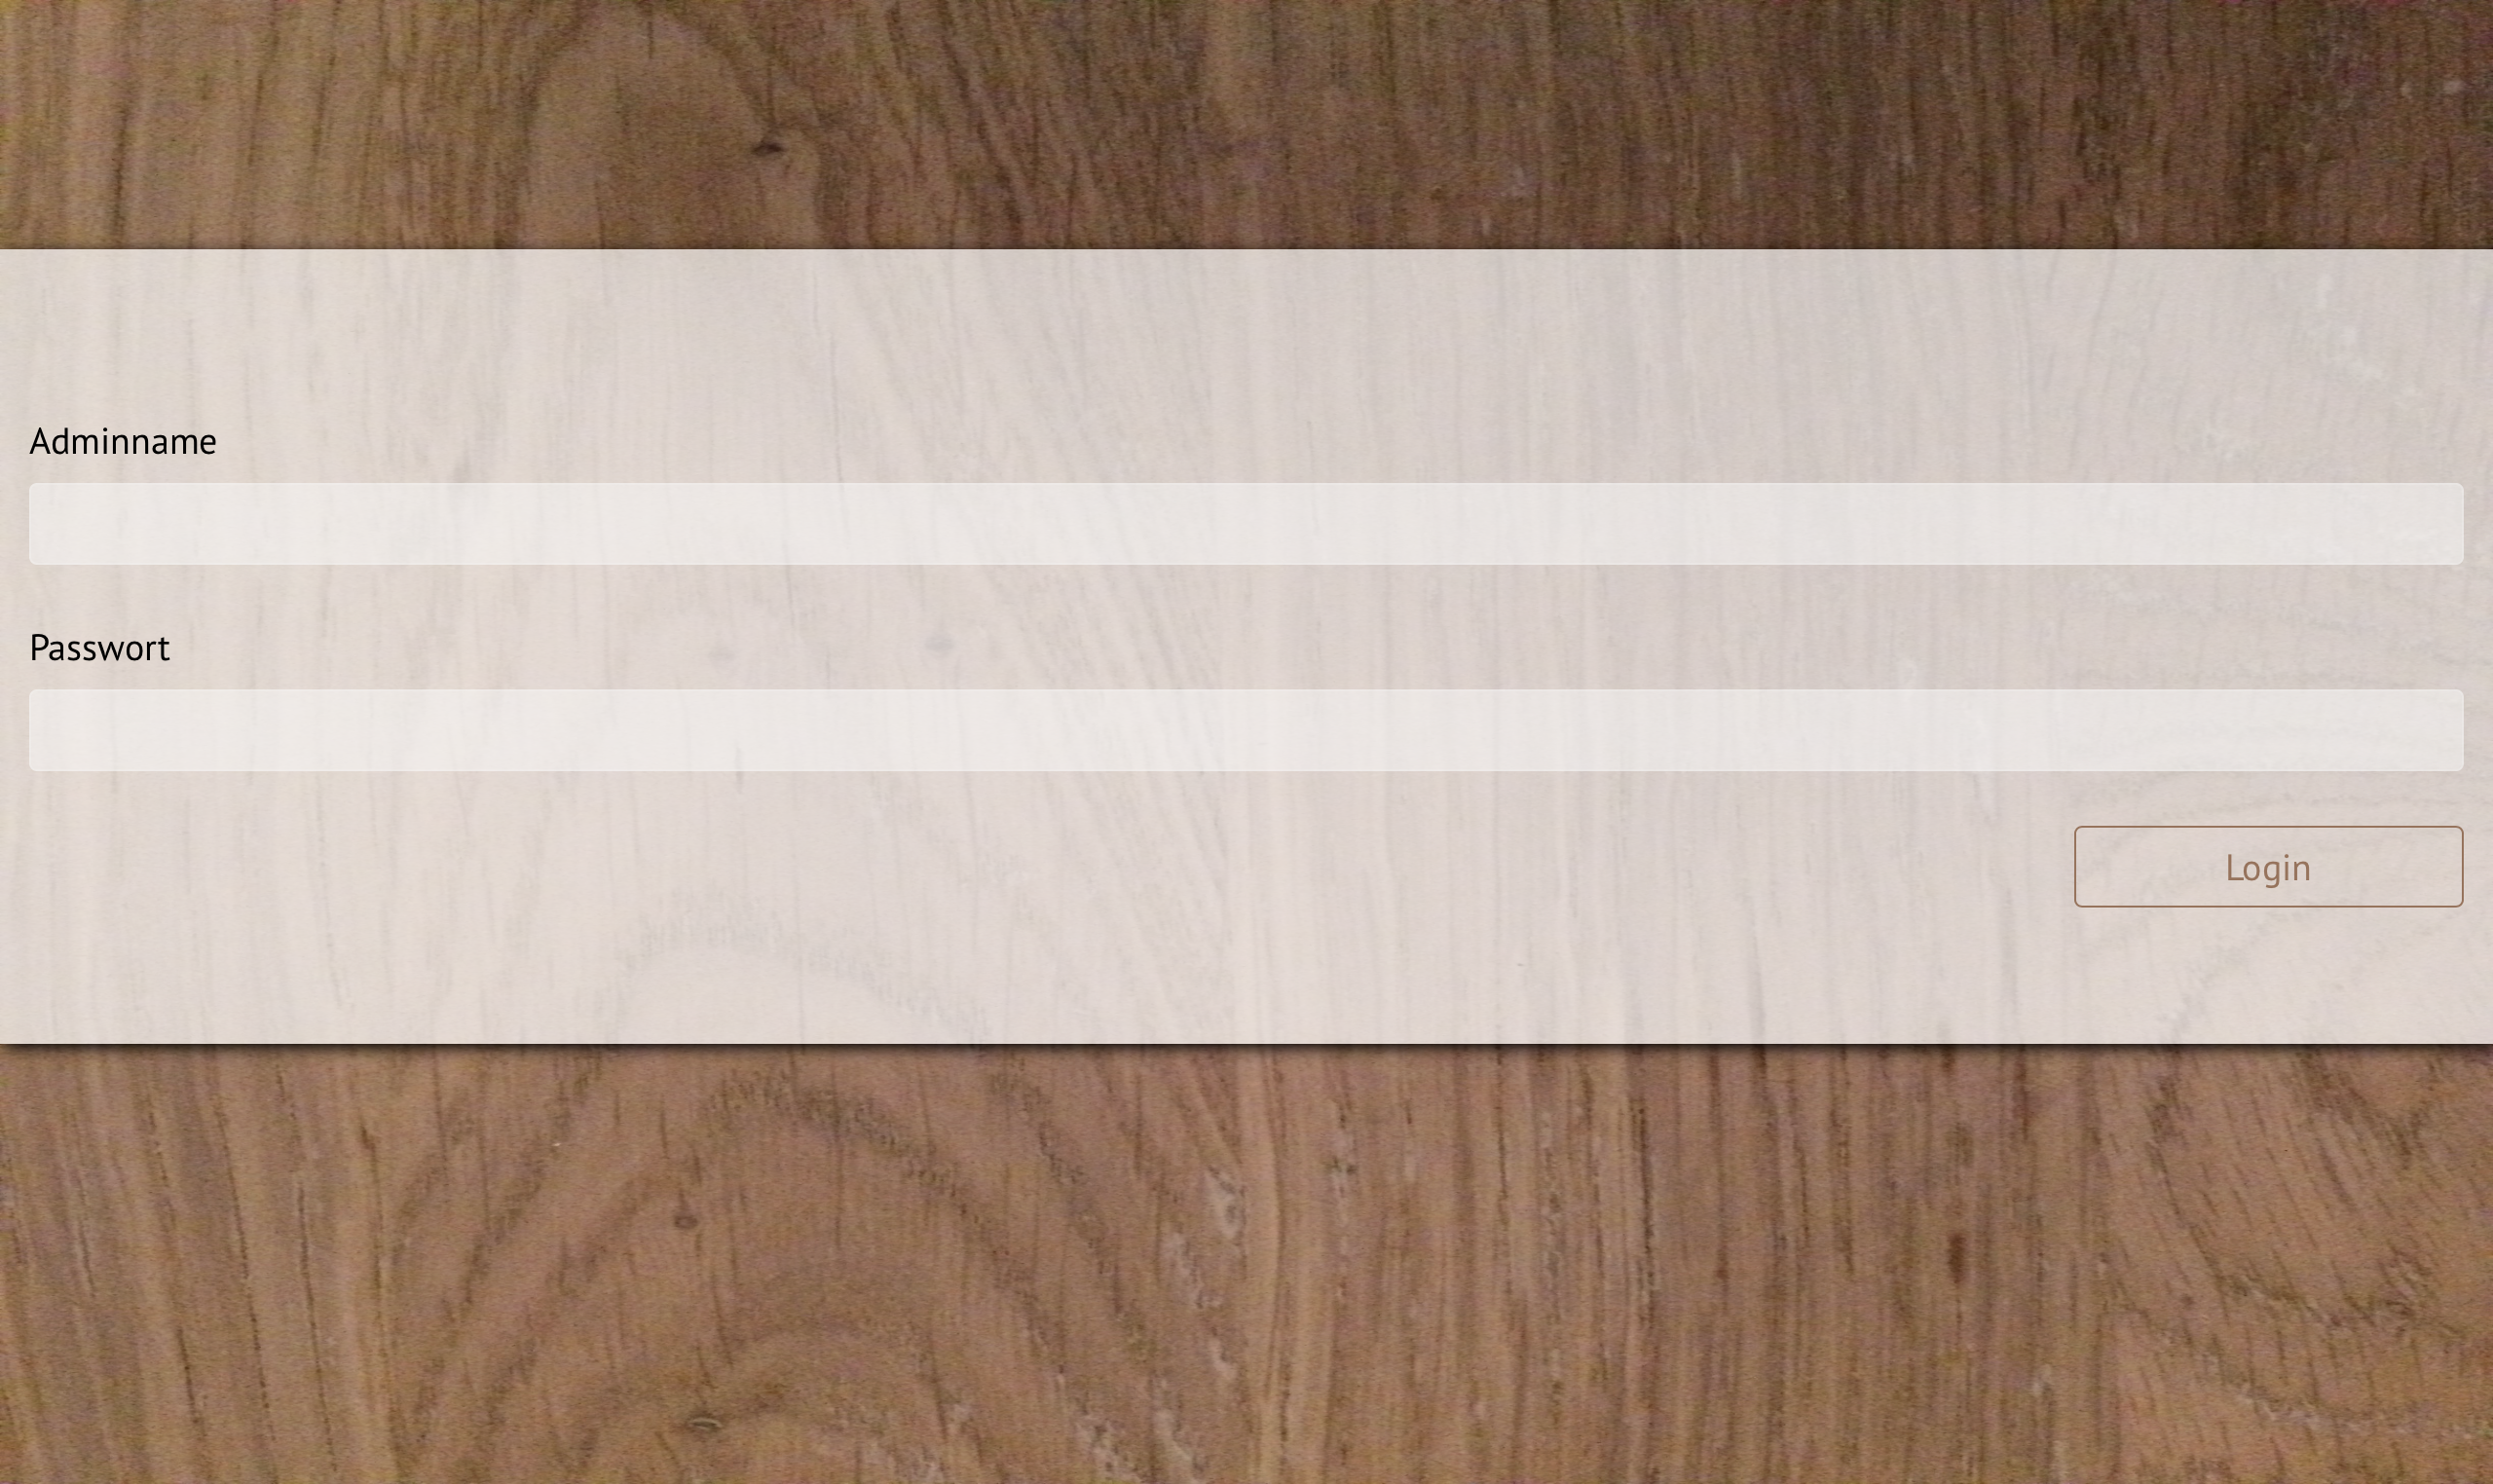
\includegraphics[width = 0.9\textwidth]{Bilder/Jok_admin_login}
			\par\end{centering}
			\caption{Screen - Login}
			\label{Screen - Login}
			\end{figure}
			\begin{figure}[H]
			\begin{centering}
			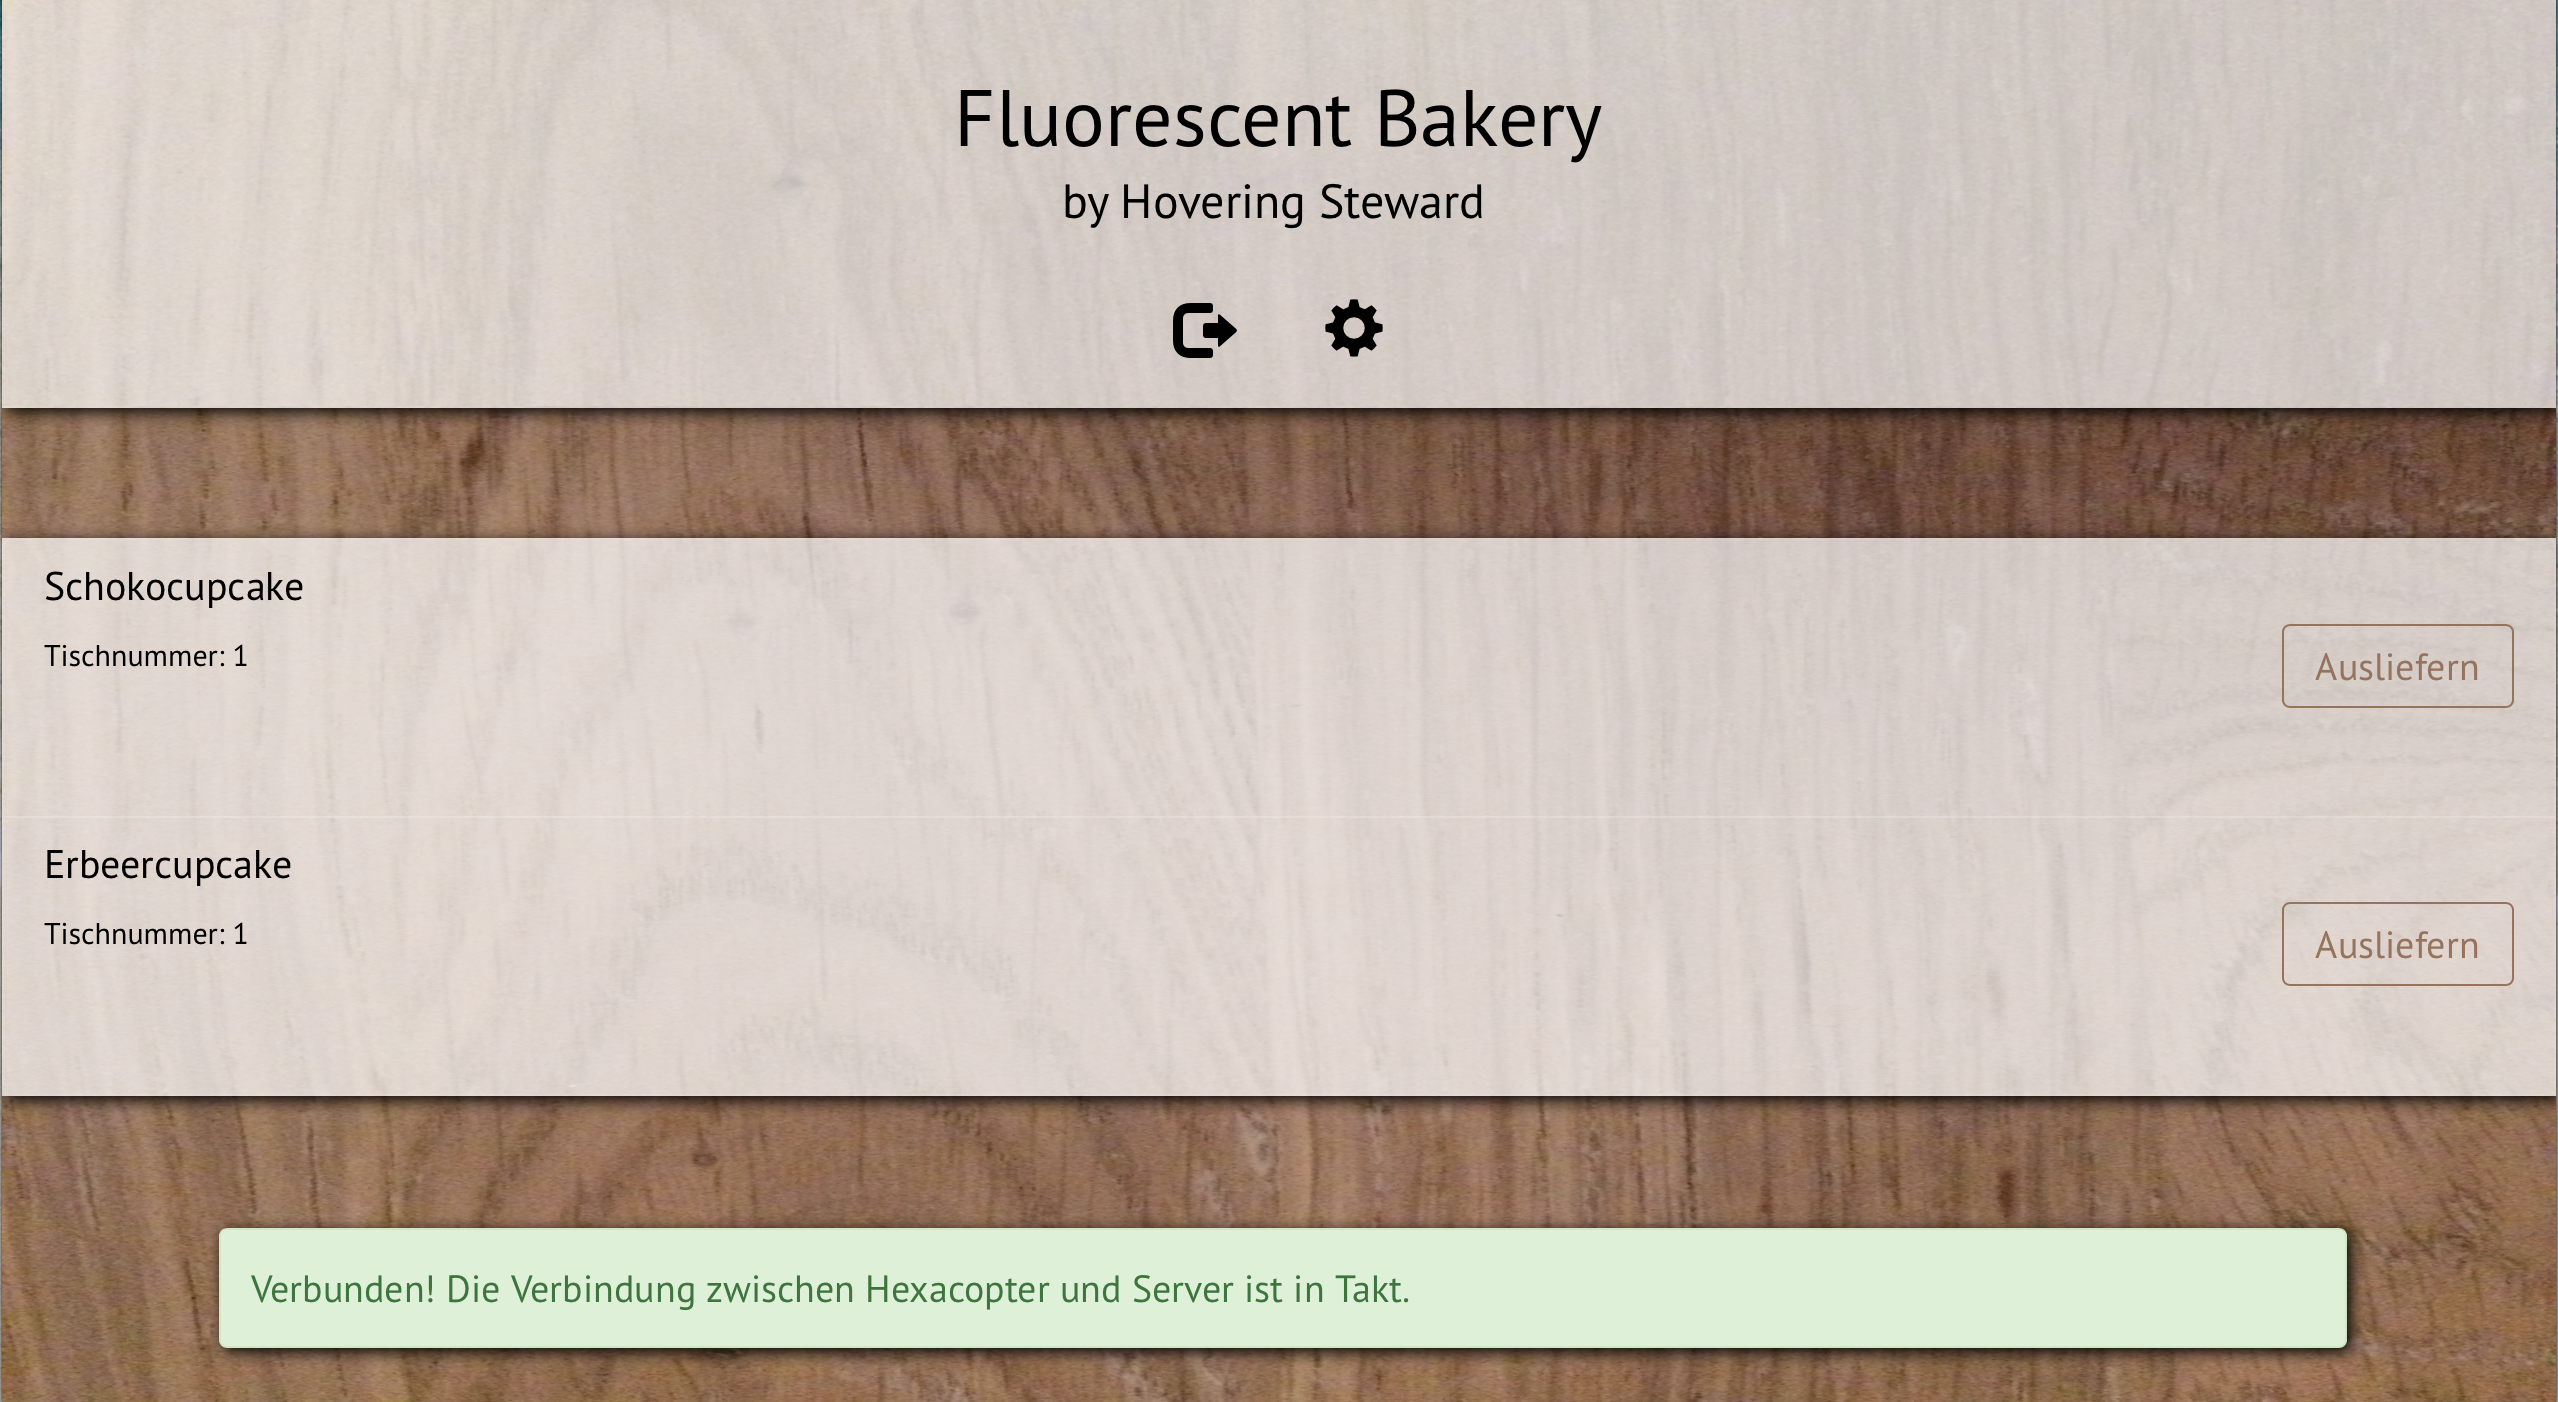
\includegraphics[width = 0.9\textwidth]{Bilder/Jok_admin_hauptscreen}
			\par\end{centering}
			\caption{Screen: Hauptscreen}
			\label{Screen: Hauptscreen}
			\end{figure}  
			\begin{figure}[H]
			\begin{centering}
			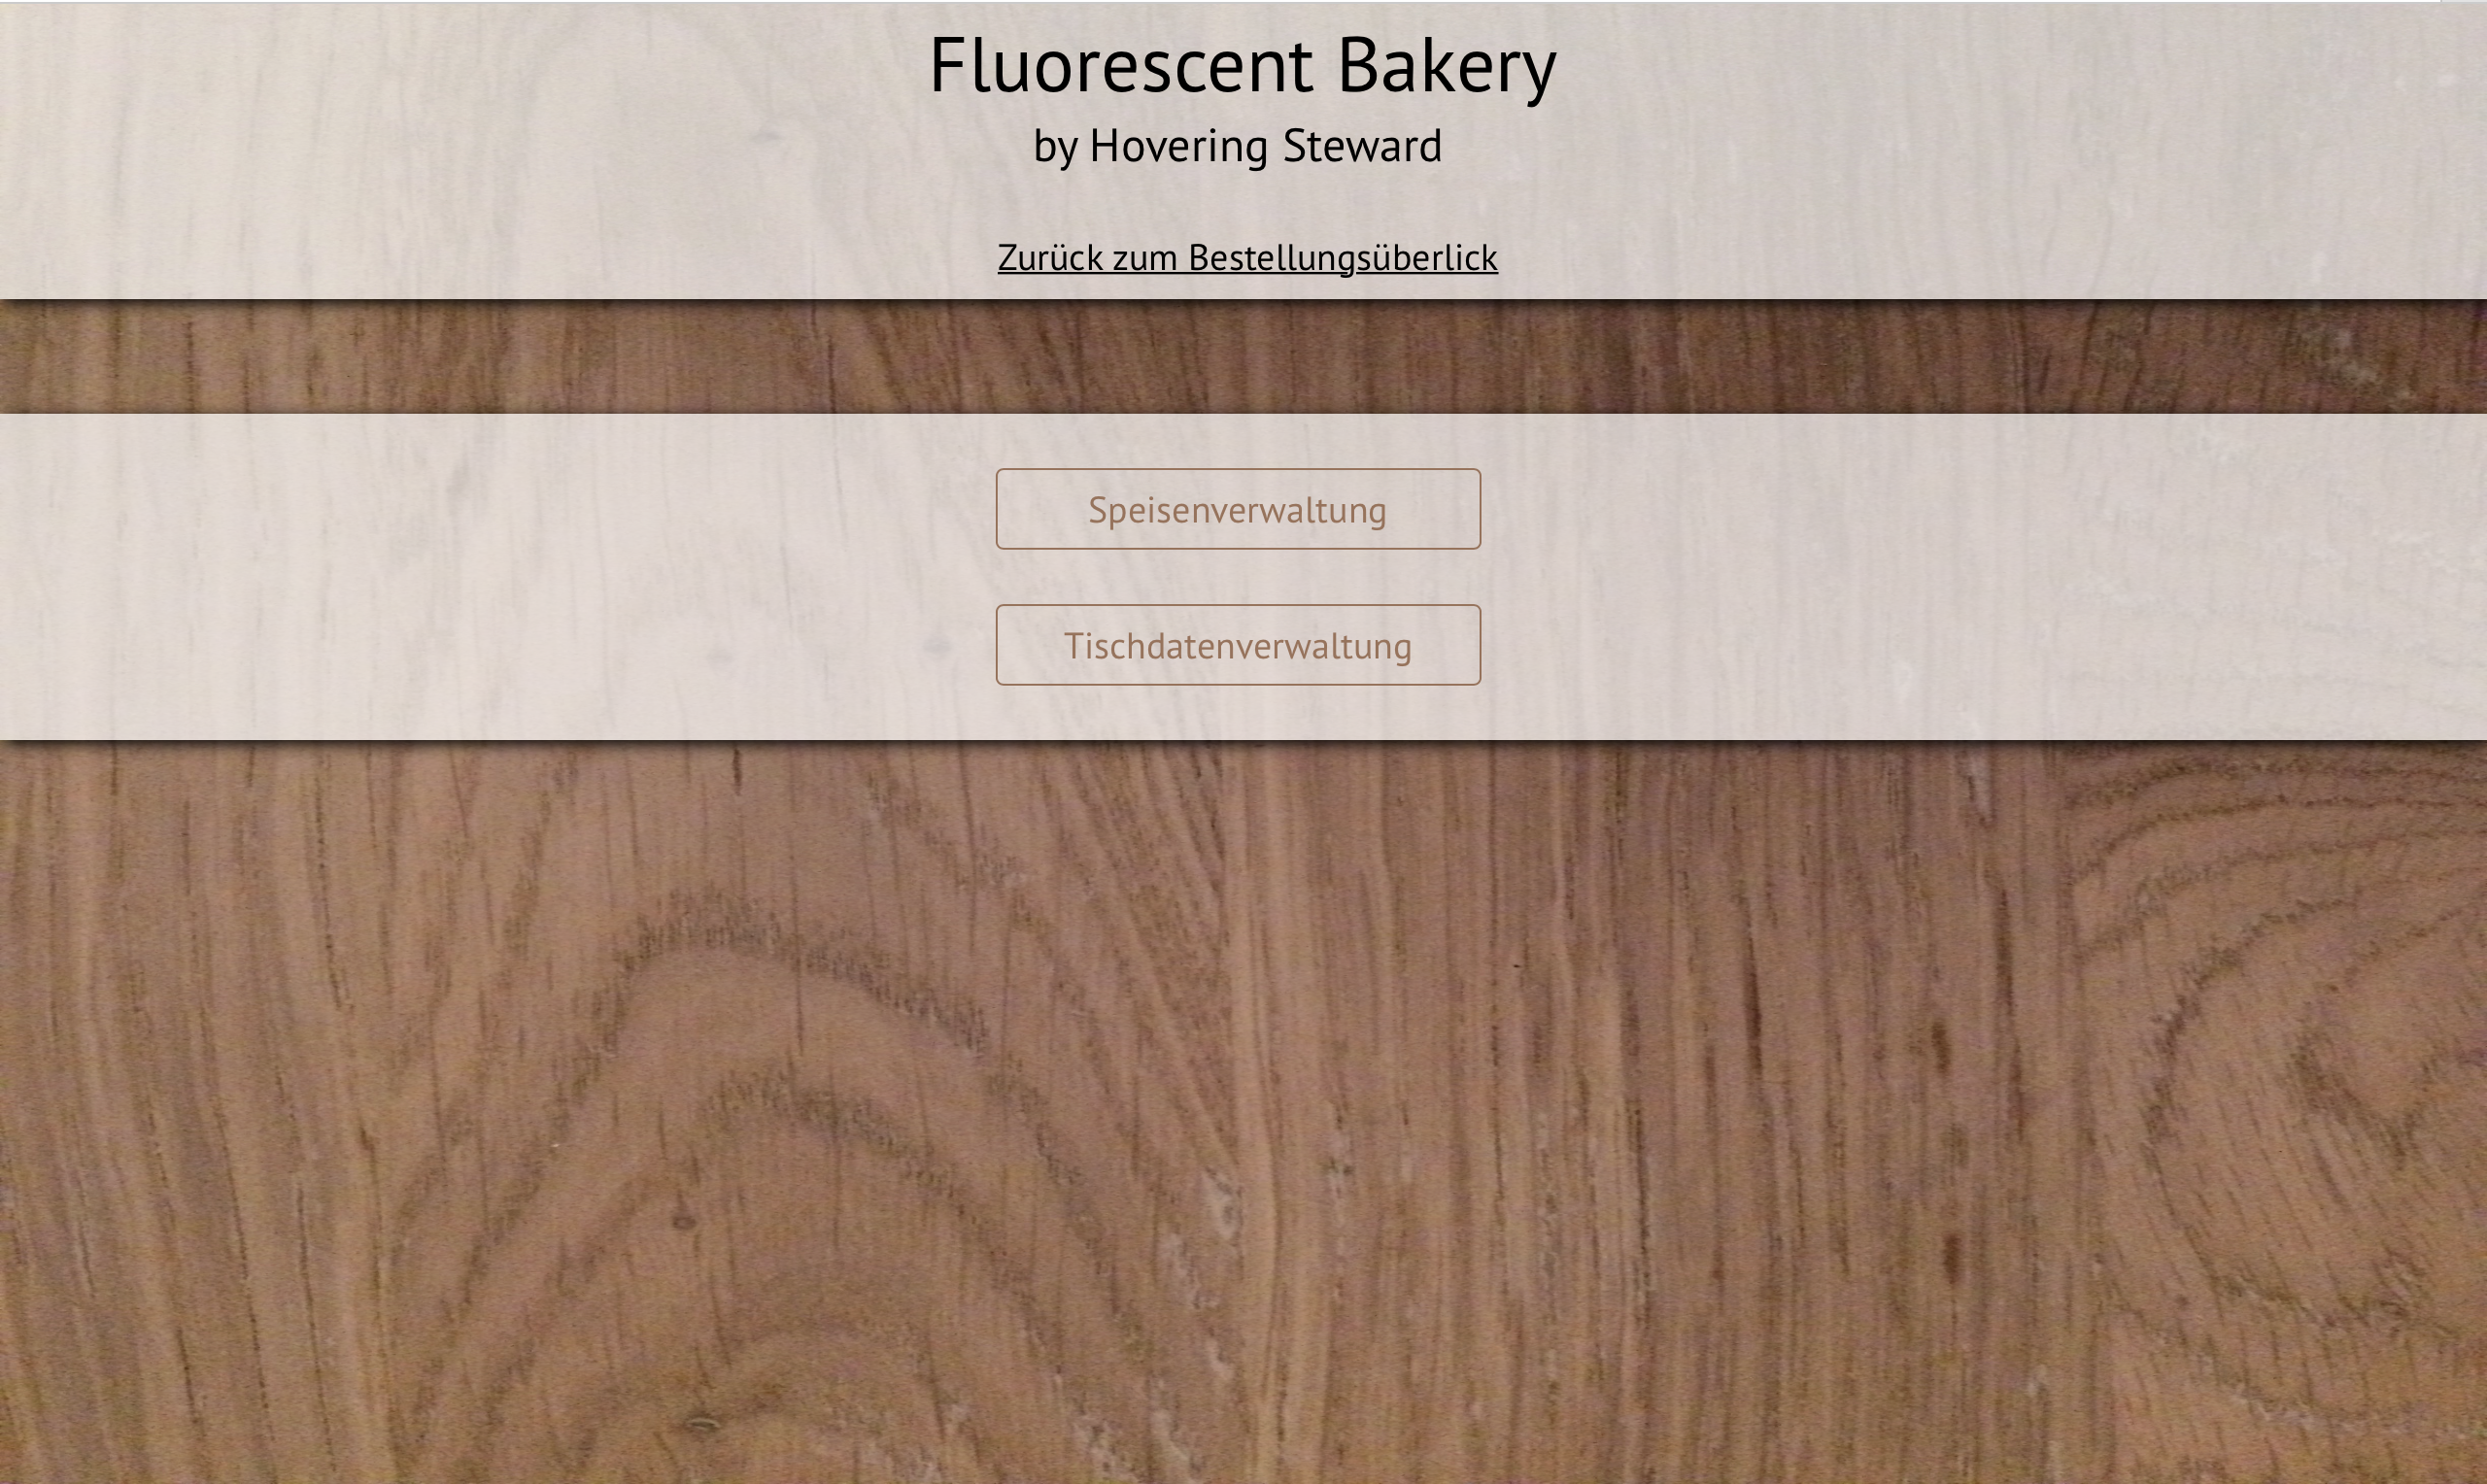
\includegraphics[width = 0.9\textwidth]{Bilder/Jok_admin_einstellungsueberblick}
			\par\end{centering}
			\caption{Screen: Einstellungsüberblick}
			\label{Screen: Einstellungsüberblick}
			\end{figure}  
			\begin{figure}[H]
			\begin{centering}
			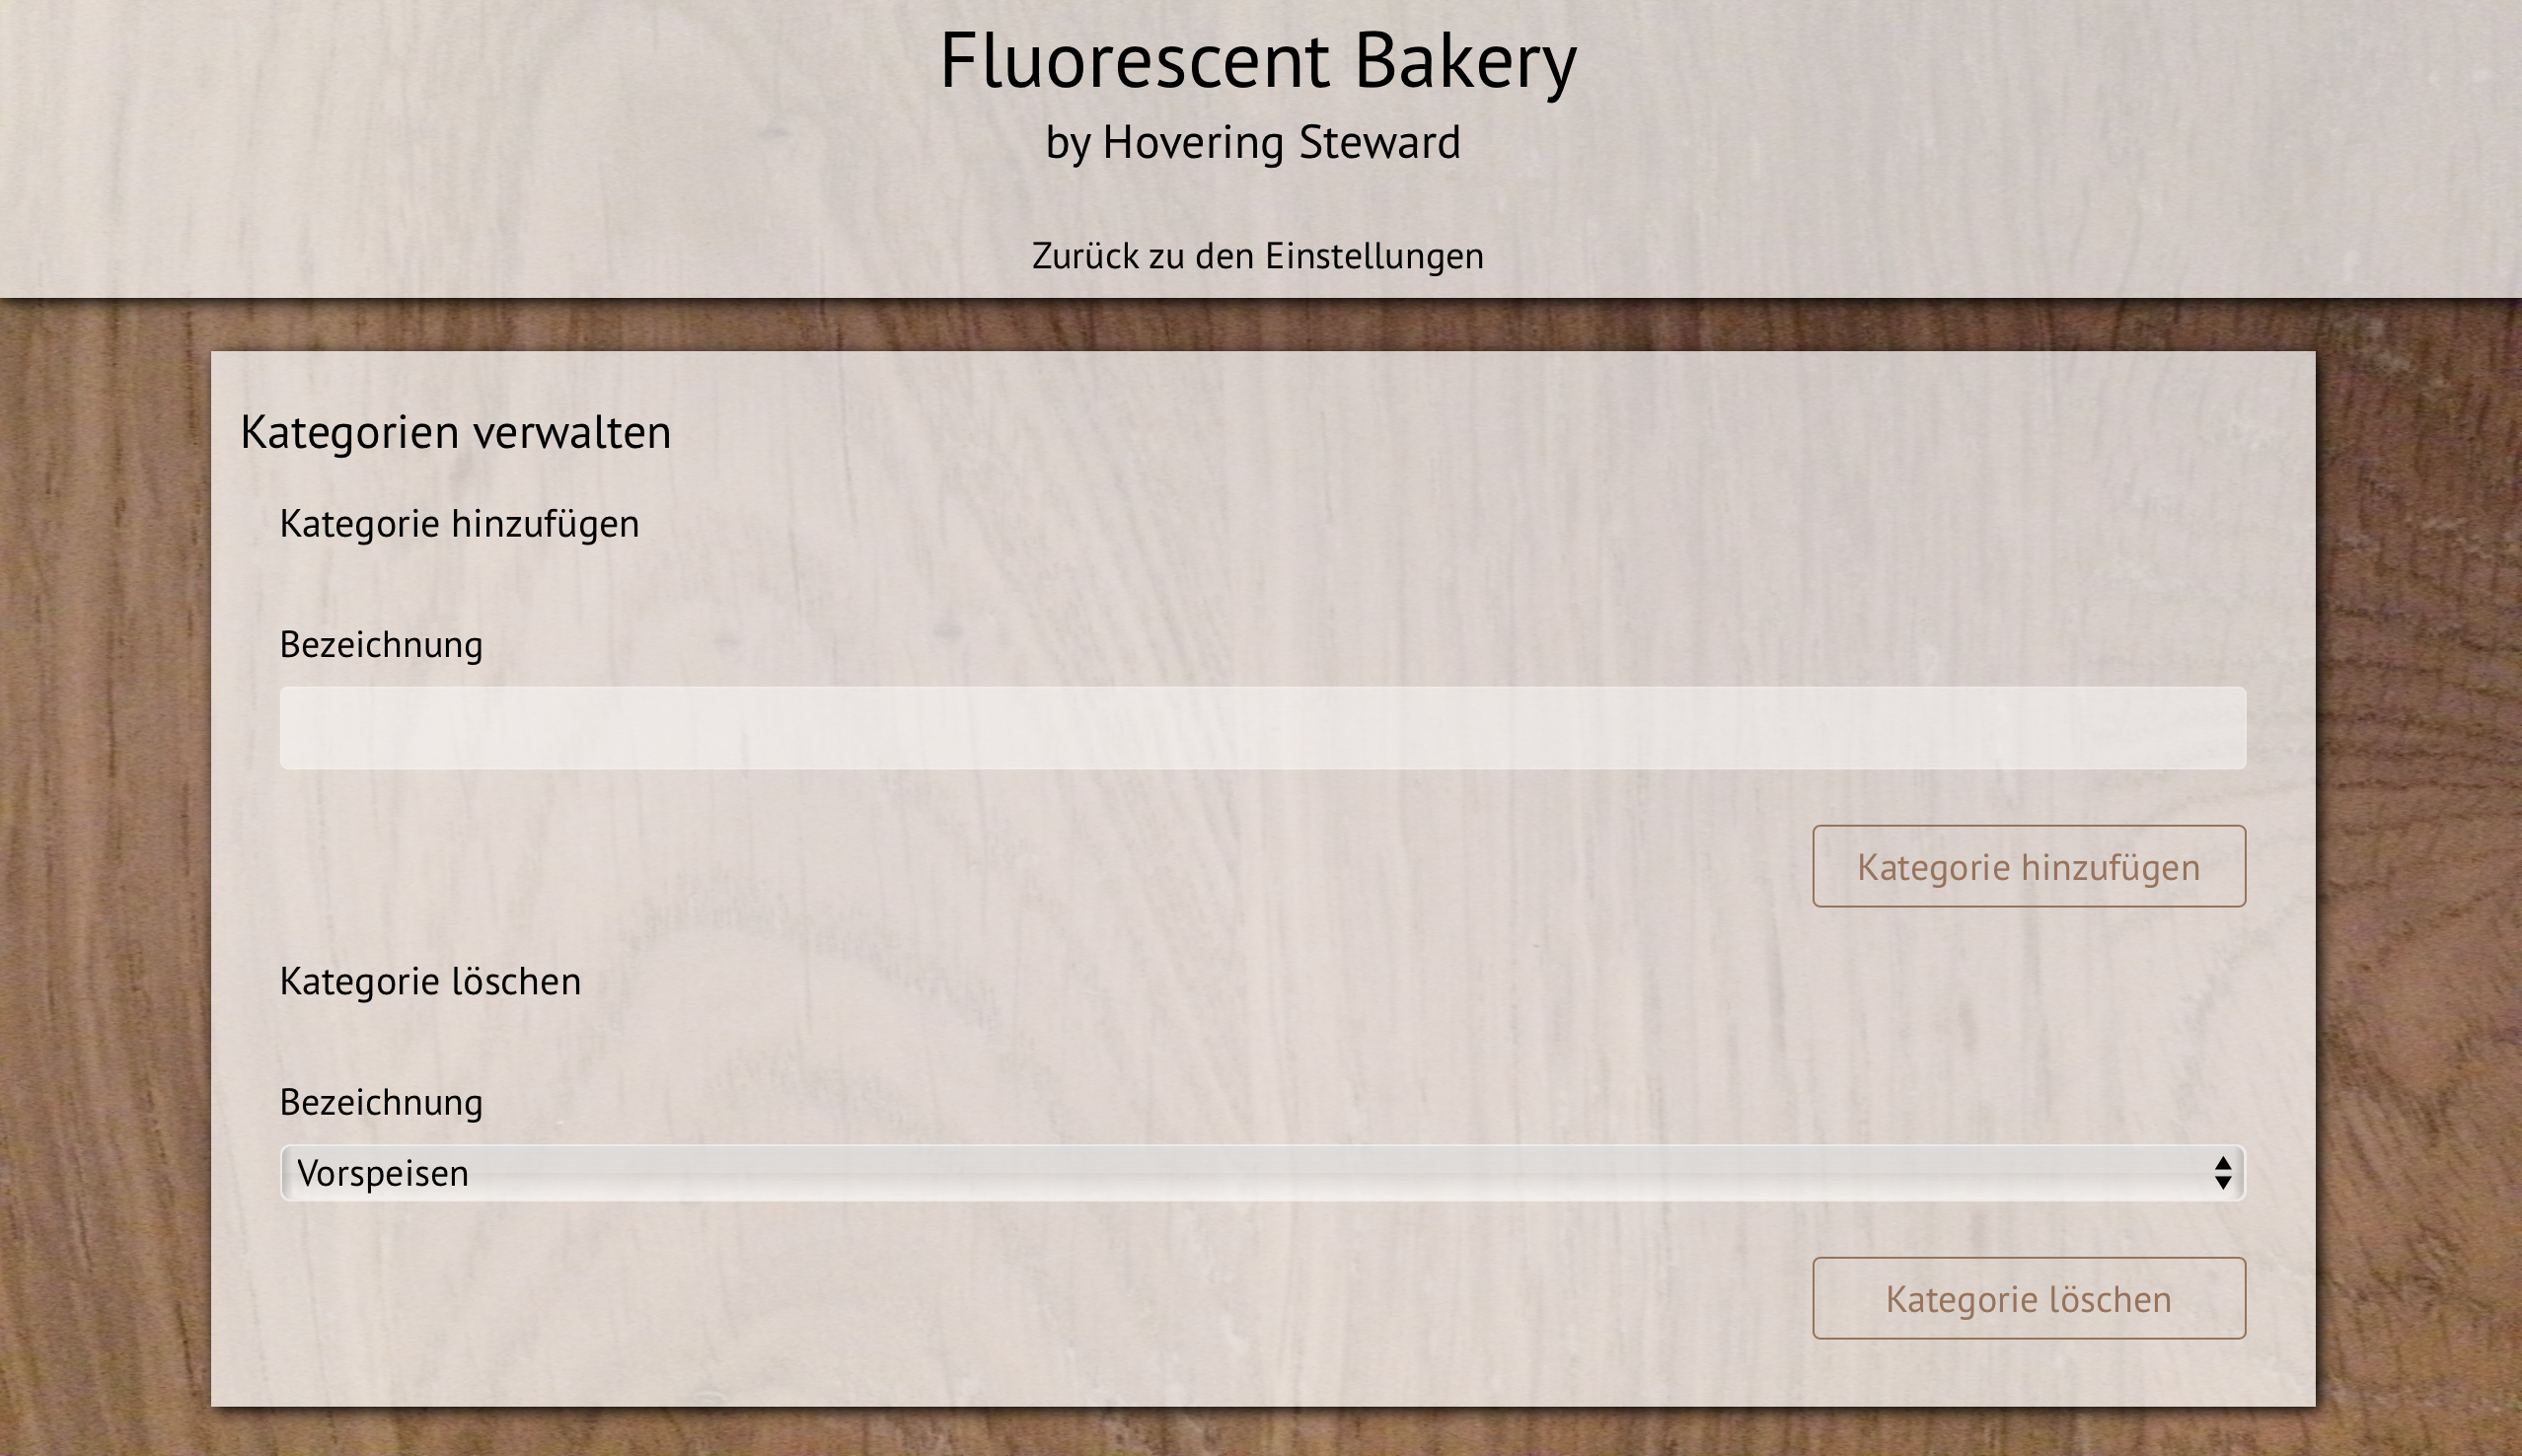
\includegraphics[width = 0.9\textwidth]{Bilder/Jok_admin_speiseverwaltung}
			\par\end{centering}
			\caption{Screen: Speise- und Kategorieverwaltung}
			\label{Screen: Speise- und Kategorieverwaltung}
			\end{figure}  
			\begin{figure}[H]
			\begin{centering}
			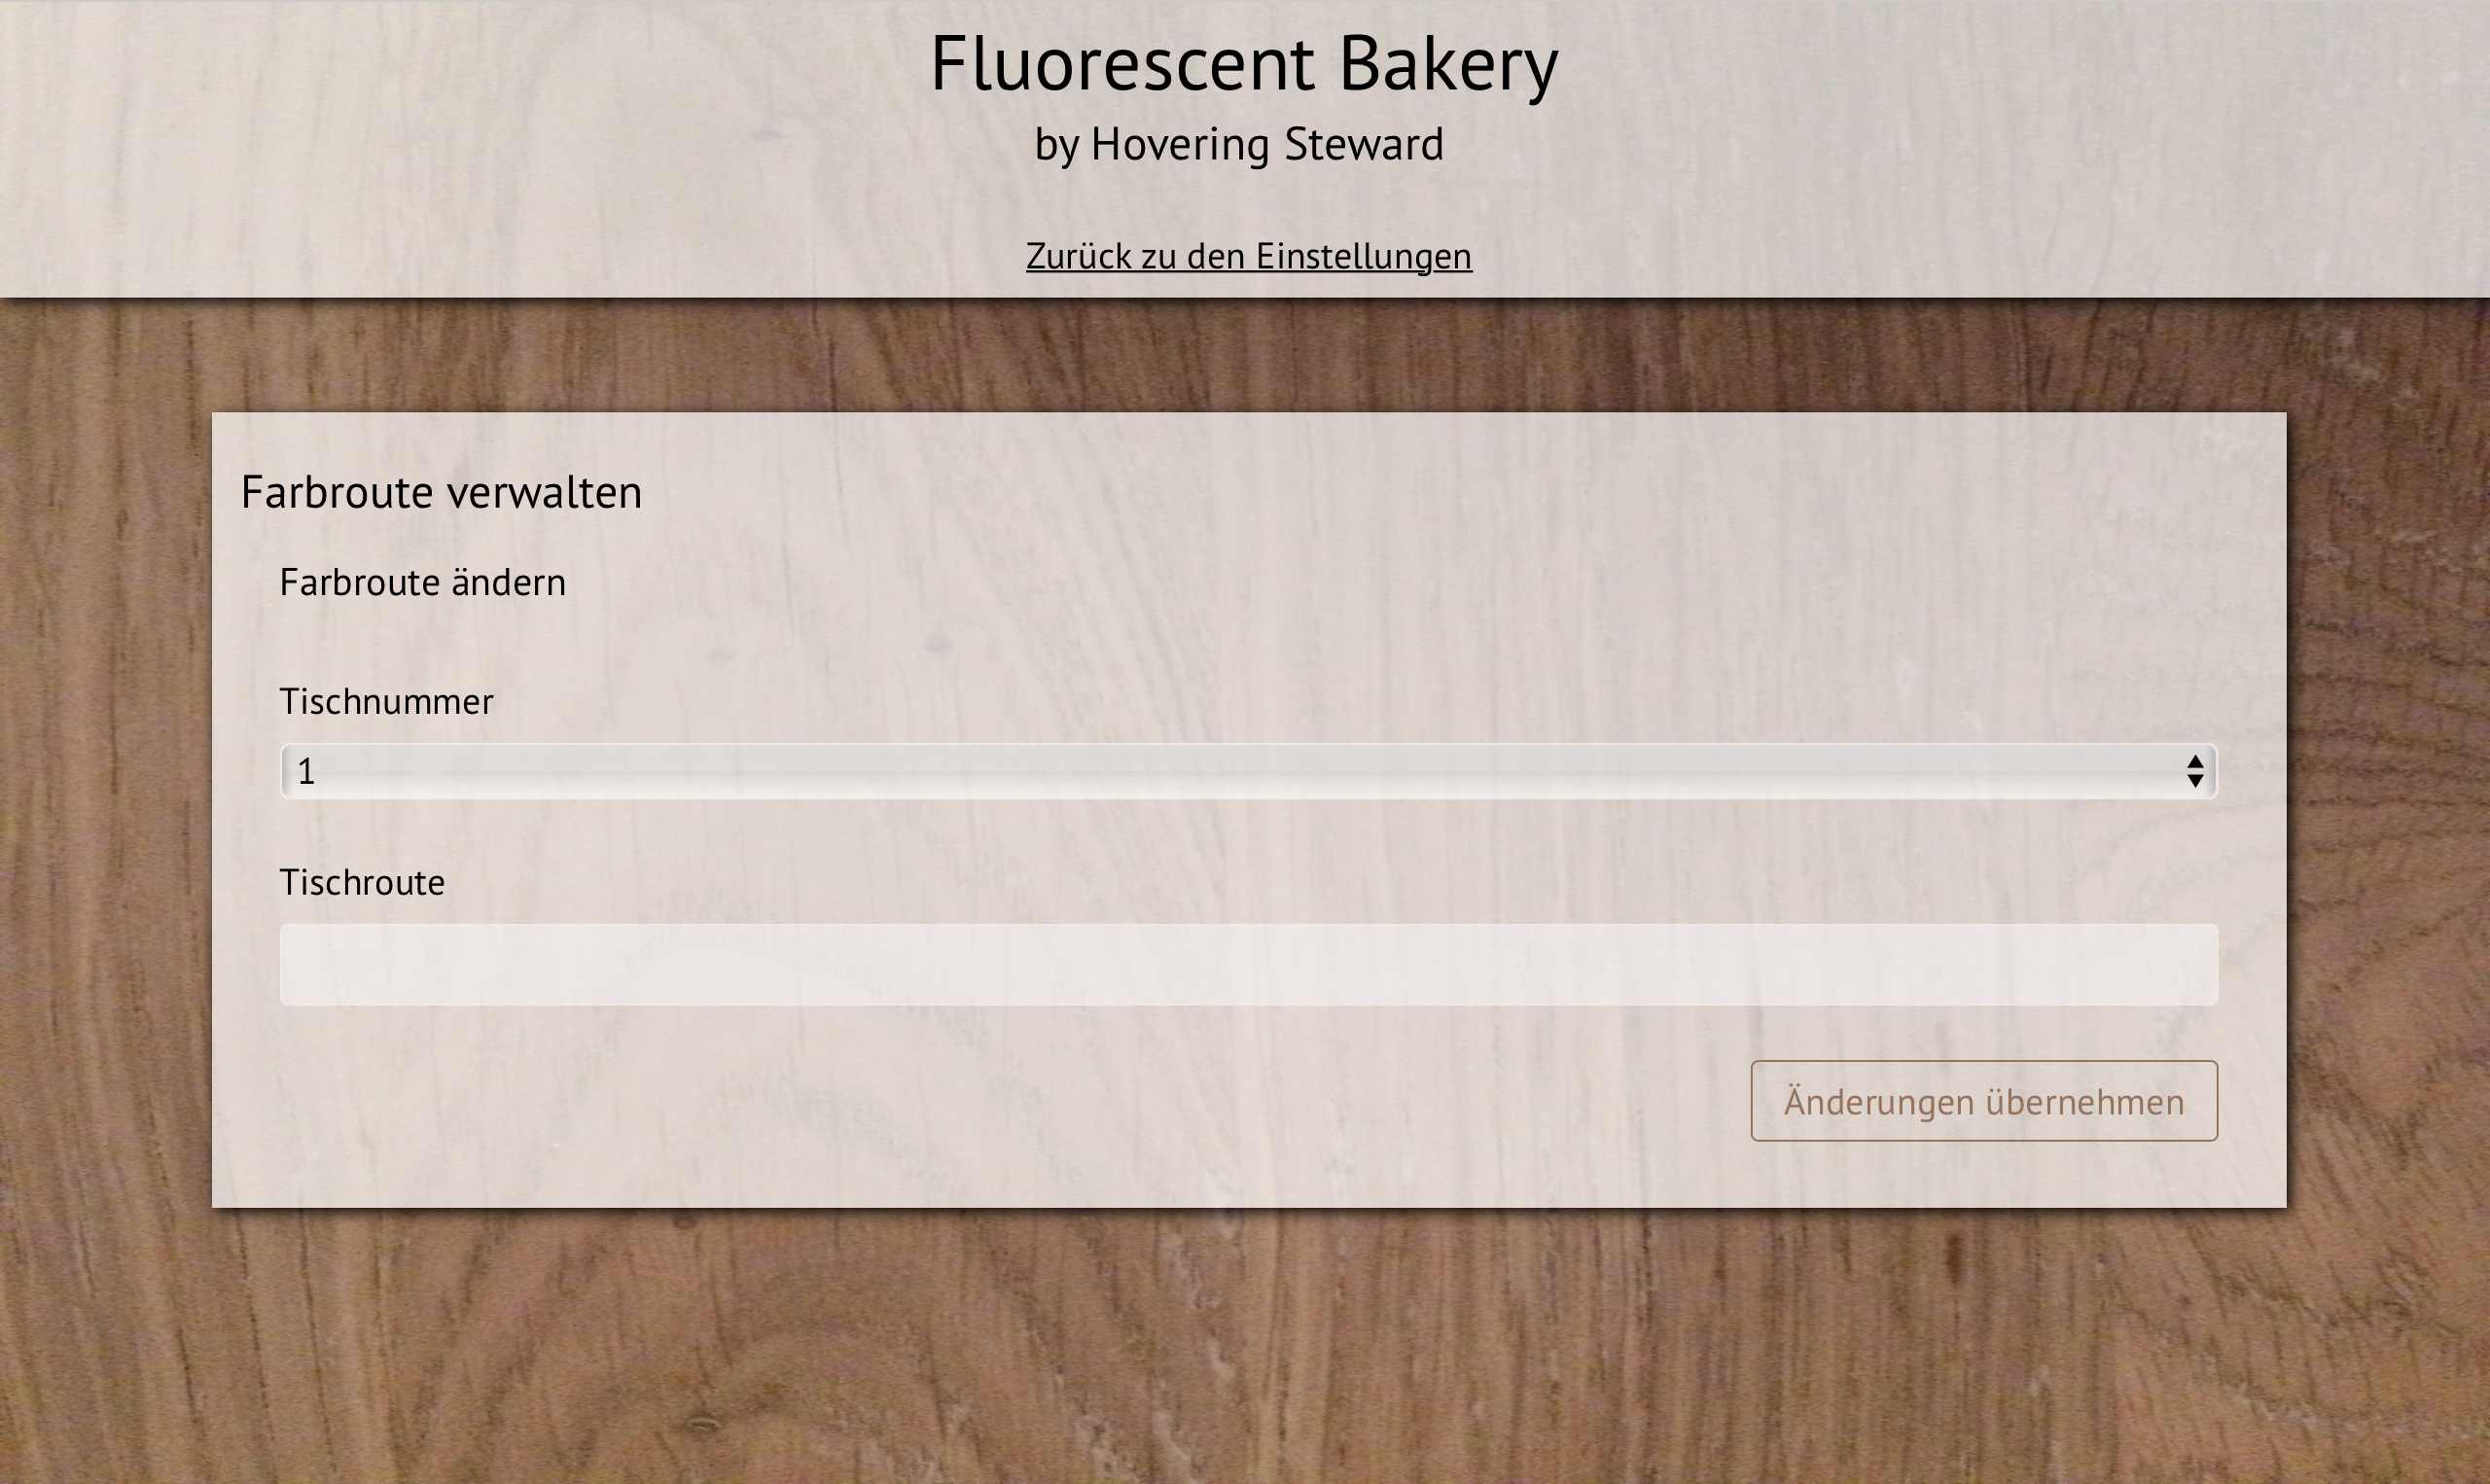
\includegraphics[width = 0.9\textwidth]{Bilder/Jok_admin_tischdaten}
			\par\end{centering}
			\caption{Screen: Tischdatenverwaltung}
			\label{Screen: Tischdatenverwaltung}
			\end{figure}  				
    \subsubsection{Datenausgabe}

Wie bereits zuvor erwähnt wurde, ermöglicht die Template Engine Twig einen vereinfachten Zugriff auf die Variablen, welche vom Controller übergeben wurden. Um eine einzige Variable aufzurufen, musste diese lediglich mit zwei geschwungenen Klammern umhüllt werden. 
\lstset{language = php}
  	\begin{lstlisting}
{{ VARIABLEN_BEZEICHNUNG }}
\end{lstlisting}
Hierbei kann über den beliebig gewählten Namen, welchen man beim Rückgabewert der Action-Funktion mitgeliefert hat, auf die Variable zugegriffen werden. 
Falls die Variable mit einem herkömmlichen String verbunden werden soll, wird eine Tilde als Verknüpfungszeichen benötigt. 
\lstset{language = php}
  	\begin{lstlisting}
var STRING_BEZEICHNUNG= {{ VARIABLEN_BEZEICHNUNG }}~"TEXT";
Die Variable kann allerdings auch problemlos in einer von Twig zur Verfügung gestellten IF-Anweisung verwendet werden.
Um die Datenbankdaten der digitalen Speisekarte auslesen zu können, wurde die von Twig mitgelieferte Art Schleifen zu generieren verwendet. Damit die Tabellenspalten einzeln angezeigt werden konnten, musste an die Bezeichnung des aktuellen Tabelleneintrags einfach die Spaltenbezeichnung angehängt werden. 
\lstset{language = php}
  	\begin{lstlisting}

	{{ AKTUELLER_TABELLENEINTRAG.SPALTEN_BEZEICHNUNG }}

	\end{lstlisting}
Falls eine Relation zu einer anderen Datenbanktabelle besteht, wie zum Beispiel beim Zugriff auf die Speiseeinträge der jeweiligen Kategorien, musste im Aufruf ebenfalls auf diese verwiesen werden, bevor der auszugebende Wert von ihr geholt werden konnte.
\lstset{language = php}
  	\begin{lstlisting}

{{ AKTUELLER_TABELLENEINTRAG.VERLINKTE_TABELLE.SPALTENBEZEICHNUNG }}

	\end{lstlisting}
Bei Werten, welche auf diese Art und Weise von der Datenbank geholt werden, wurde darauf geachtet, dass sie kompatibel für Textausgaben kodiert wurden. Dies wird am besten mit einer JSON-Kodierung bewerkstelligt.
\lstset{language = php}
  	\begin{lstlisting}
var VARIABLEN_BEZEICHNUNG = 
{{ AKTUELLER_TABELLENEINTRAG.SPALTENBEZEICHNUNG|json_encode|raw  }};
	\end{lstlisting}
Mit diesem Schema konnten alle Speisekarteninformationen in dem Frontend der Applikation angezeigt werden.

    \subsubsection{Formulargenerierung}

Um das Formular, welches über den Controller übermittelt wurde, anzeigen zu können, musste in der Twig-Datei nicht mehr viel erledigt werden. Hier galt es nur noch, die bereits definierten Eingabefelder aufzurufen und ihnen nach Belieben Attribute zuzuteilen.
\lstset{language = java}
  	\begin{lstlisting}
{{ form_start(FORMULAR_BEZEICHNUNG) }}
            {{ form_label(FORMULAR_BEZEICHNUNG.FORMULARFELD_BEZEICHNUNG}}
            {{ form_widget(FORMULAR_BEZEICHNUNG.FORMULARFELD_BEZEICHNUNG, 
            {'attr': {'ATTRIBUT_BEZEICHNUNG': 'ATTRIBUT_WERT'}}) }}
{{ form_end(FORMULAR_BEZEICHNUNG) }}
	\end{lstlisting}
Um dem Template mitzuteilen, dass die Generierung eines Formulars gestartet werden soll, musste die "start()"-Funktion aufgerufen und ihr die Bezeichnung des Formulars, welche im Rückgabewert der Actionfunktion im Controller definiert wurde, als Parameter mitgeschickt werden. 
Anschließend kann auf alle Felder und Labels des Formulars zugegriffen werden. Es empfiehlt sich zuerst das Label mit der "label()"-Methode, welche sowohl die Bezeichnung des Formulars als auch die des Eingabefelds übergeben werden sollen, und anschließend erst das Eingabefeld mit der "widget()"-Funktion, der dieselben Parameter übermittelt werden sollen, abzurufen. Es gibt die Möglichkeit jedem Label und Eingabefeld Attribute zuzuteilen um sie beliebig zu gestalten. Im Frontend werden alle Formularelemente gleich behandelt, da bereits im Controller die spezifischen Funktionalitäten zugewiesen wurden. Das heißt die Generierung eines Buttons in einer Twig-Datei unterscheidet sich nicht von der eines Texteingabefeldes.
Mit diesem Codeschema wurden alle Login-, Speisen- und Tischdatenverwaltungsformulare visuell dargestellt.

  \subsection{Herausforderungen und Lösungen}

\textbf{Apache Zugriffsverweigerung}\\ 
Damit die Applikation über den Apache HTTP Server im Frontend angezeigt werden kann, musste in der "app.php"-Datei angegeben werden, dass die digitale Speisekarte auch in einer Produktionsumgebung, also auch im gewerblichen Gebrauch, aufgerufen werden kann und nicht nur der Symfony-Server darauf Zugriff hat.
	\lstset{language=php}
  	\begin{lstlisting}
$kernel = newAppKernel('prod', true);
  	\end{lstlisting}
Der Wert "prod" steht hierbei für "production environment", also für die Produktionsumgebung.

\section{Testphase}
Für die Testphase wurden präzise Testfälle erstellt, welche abgesehen von TC-5 von einer externen Person getestet wurden.

\begin{table}[H]
\centering
\begin{tabular}{|p{1cm}|p{3cm}|p{3cm}|p{3cm}|p{3cm}|} 
\hline \textbf{ID} & \textbf{Bezeichnung} & \textbf{Testszenario} & \textbf{Erwartetes Ergebnis} & \textbf{Erzieltes Ergebnis} \\\hline
\hline TC-1 & Adminlogin - Admininterface & Der Admin meldet sich im Adminbereich mit dem richtigen Passwort und Namen an & Hauptscreen des Admininterfaces soll angezeigt werden & Hauptscreen des Admininterfaces wird angezeigt \\\hline
\hline TC-2 & Adminlogin - Speisekarte & Der Admin meldet sich im Adminbereich mit dem richtigen Passwort und Namen an & Der Admin soll auf den Tischnummernauswahlscreen weitergeleitet werden & Der Admin wird auf den Tischnummernauswahlscreen weitergeleitet \\\hline
\hline TC-3 & Speisebestellung & Der Gast bestellt eine Speise & Ein neuer Bestellungseintrag soll erstellt werden und in der Bestellliste erscheinen & Ein neuer Bestellungseintrag wird erstellt und erscheint in der Bestellliste, nachdem in einer Alertbox die Bestellung bestätigt wurde \\\hline
\hline TC-4 & "Ausliefern"-Wert ändern & Der Admin klickt auf den "Ausliefern"-Button & Der "ausliefern"-Wert der Speise soll auf 1 gesetzt werden & Der "ausliefern"-Wert der Speise wird auf 1 gesetzt \\\hline
\hline TC-5 & Tischroute schicken & Der Hexacopter schickt eine bestimmte Nachricht an den Server & Die Tischroute soll geschickt werden & Die Tischroute wird geschickt \\\hline
\end{tabular}
\end{table}
\begin{table}[H]
\centering
\begin{tabular}{|p{1cm}|p{3cm}|p{3cm}|p{3cm}|p{3cm}|} 
\hline TC-6 & Speiseeintrag hinzufügen & Der Admin gibt neue Speisedaten in das Formular ein und klickt auf "Speiseeintrag hinzufügen" & Ein neuer Speiseeintrag soll in der Datenbank angelegt werden & Ein neuer Speiseeintrag wird in der Datenbank angelegt \\\hline
\hline TC-7 & Kategorie hinzufügen & Der Admin gibt eine neue Kategoriebezeichnung in das Formular ein und klickt auf "Kategorie hinzufügen” & Eine neue Kategorie soll in der Datenbank angelegt werden & Eine neue Kategorie wird in der Datenbank angelegt \\\hline
\hline TC-8 & Speiseeintrag löschen & Der Admin wählt einen Speiseeintrag aus und klickt auf den "Speiseeintrag Löschen"-Button & Der ausgewählte Speiseeintrag soll gelöscht werden & Der ausgewählte Speiseeintrag wird gelöscht \\\hline
\hline TC-9 & Kategorie löschen & Der Admin wählt eine Kategorie aus und klickt auf den "Kategorie Löschen"-Button & Die ausgewählte Kategorie soll gelöscht werden & Die ausgewählte Kategorie wird gelöscht \\\hline
\hline TC-10 & Tischroute verändern & Der Admin wählt eine Tischnummer aus und gibt eine Tischroute in das Formularfeld ein & Die Tischroute des Tisches mit der ausgewählten Tischnummer soll geändert werden & Die Tischroute des Tisches mit der ausgewählten Tischnummer wird geändert \\\hline
\end{tabular}
\caption{Testfälle der Applikation und des Java Programms}
\end{table}

\section{Persönliche Erfahrungen}
Da ich zuvor kaum mit einer der hierfür verwendeten Technologien gearbeitet habe, konnte ich mir dank der Diplomarbeit einige neue Fähigkeiten erlernen.
Zwar habe ich bereits in der vierten Klasse die Grundlagen eines MVC-Frameworks gelernt, doch war mir damals trotzdem kaum klar, wie es genau funktioniert und wie viele positive Eigenschaften es eigentlich mit sich bringt.
Zuerst dachte ich, dass es mehr Aufwand mit sich bringen würde, da ich mich nicht gut damit auskannte, doch mittlerweile ist die Verwendung von Symfony für mich kaum noch wegzudenken. Ohne diesem Framework, hätte ich mich vermutlich kaum in meiner Codestruktur zurechtgefunden.
So ging es mir jedoch nicht nur mit Symfony sondern nahezu mit jeder anderen Technologie die verwendet wurde auch. 
Ich habe zwar ziemlich viel Zeit dafür aufgebracht mit Doctrine zurechtzukommen, doch dies hat sich auf jeden Fall ausgezahlt. Dadurch konnte ich nämlich Änderungen in der Datenbank ohne großen Aufwand vornehmen. 
Ich bin wirklich froh darüber, dass ich mit der Template Engine Twig gearbeitet habe, da ich dadurch keinen aufwendigen Code in den Dateien für die visuelle Darstellung zur Ausgabe von Variablen eingeben musste, sondern lediglich wenige Zeilen mit dem Twig-Syntax angeben konnte.
\\
Dadurch, dass wir uns im Projektteam zu Beginn der Diplomarbeit kaum kannten, führten wir Coachings ein, welche regelmäßig stattfanden. In diesen wurde der Fokus neben der Planung des Projekts auch immer wieder auf das Zusammenschweißen der Teammitglieder gelegt. Dadurch kann ich mittlerweile wirklich behaupten, dass wir fünf uns nun prima miteinander verstehen und auch längere Zeit miteinander auskommen ohne dass es zu Streitigkeiten kommt. Wir können alle offen miteinander über Probleme reden und uns darauf verlassen, dass jeder dem anderen bei Schwierigkeiten mit Rat oder Motivation zur Seite steht.
\\
Mein persönliches Fazit ist, dass ich dank dieser Diplomarbeit meinen Wissenshorizont um ein Vielfaches erweitert habe und auch, dass meine sozialen Kompetenzen davon profitiert haben. 

\section{Ergebnisse}
Sowohl die Screens der digitalen Speisekarte als auch die des Admininterfaces sind funktionstüchtig.
Das Java Programm bietet ebenfalls wie im optionalen Ziel definiert, die Möglichkeit die Tischroute automatisch an den Hexacopter schicken zu können.


% !TEX root = diplomarbeit.tex
\chapter{Positionierung}
\renewcommand{\kapitelautor}{Autor: Christina Bornberg}

%%%%%%%%%%%%%%%%%%%%%%%%%%%%%%%%%%%%%%%%%%%%%%%%%%%%%%%%%%%%%%%%%%%%%%%%%%%%%%%
\section{Allgemeine technische Planung}

    \subsection{Allgemein}
    Um eine Positionsbestimmung durchzuführen, wird ein Trackingsystem benötigt.
    Es gibt mehrere Verfahren, um ein Objekt zu tracken: \cite{PositionAllg}
    \begin{itemize}
    \item Mechanische Systeme, umgesetzt mit einer mechanischen Verbindung
    \item Elektromagnetisches Tracking, umgesetzt mit elektromagnetischen Wellen
    \item Akustisches Tracking, umgesetzt mit akustischen Wellen
    \item Optisches Tracking, umgesetzt mit elektromagnetischen Wellen
    \item Inertial Tracking, umgesetzt mit Beschleunigungsmessern und Gyroskopen
    \item hybride Ansätze, umgesetzt mit Kombinationen, die mehrere Systeme vereinen
    \end{itemize}
    Elektromagnetische, optische und akustische Verfahren werden in späteren Abschnitten genauer behandelt.

    \subsection{Anwendung}
    Indoor Positionierungssysteme werden derzeit vor allem zur Objekterkennung, im Umweltmonitoring, über das Detektieren von Bränden in Gebäuden, bis hin zum Einsatz in der Logistik, verwendet. Da es sehr viele unterschiedliche Anwendungsgebiete gibt, werden unterschiedliche Methoden verwendet. \cite{posAnwendung}

    \subsection{Eigenschaften der Positionsbestimmung}

    Ein Positionierungssystem kann verschiedene Arten von Informationsdaten aufweisen. \cite{pos_eigenschaften}

    \subsection*{Physische und symbolische Positionierung}
    Die \textbf{physische Positionierung} ist eine exakte Position, die zum Beispiel in einem Koordinatensystem, meist in 2-D oder 3-D Karten, bestimmt wird. Längen- und Breitengrade spielen dabei eine wichtige Rolle.\\
    \textbf{Symbolische Positionierung} ist die abstrakte Beschreibung eines Ortes, sie wird sprachlich beschrieben, beispielsweise Küche, Garten, Dachboden.\\
    Eine physikalische Position kann auch symbolisch beschrieben werden.

    \subsection*{Relative und absolute Positionierung}
    Autor: Lucas Ullrich\\

    \textbf{Absolute Positionsmessung}\\
    Hier wird die Position von einem gleichbleibenden Bezugspunkt aus gemessen. Dabei ist ein konstanter Referenzpunkt wichtig.
    Verändert sich dieser oder kann die Distanz nicht genau gemessen werden ist die Messung unbrauchbar.

    Für eine absolute Positionsmessung bieten sich diverse Triangulationsverfahren an, diese sind ausgesprochen rechenaufwändig und benötigen meist eine sehr genaue Laufzeitmessung.
    Für die Triangulation können die unterschiedlichsten Signale verwendet werden, am gängigsten sind jedoch jene die mit elektromagnetischen Wellen arbeiten,
    zum Beispiel WLAN, Bluetooth. Dies bedeutet, dass sich die Signale mit Lichtgeschwindigkeit ausbreiten.

    Bei einer Messung derart schneller Signale muss ein hoher Aufwand betrieben werden um eine Messgenauigkeit von einigen cm zu erzielen.

    Eine weitere Herausforderung sind Hindernisse wie Mauern. Hier muss ständig berücksichtigt werden wo ein Objekt steht und ob der geplante Weg überhaupt frei ist.

    \textbf{Relative Positionsmessung}\\
    Hier wird die Position von einem wechselnden Punkt aus gemessen. Um hier eine Positionierung im Raum ermöglichen zu können,
    ist es erforderlich immer zu einem bestimmten Punkt zu messen. Ein Wechsel dieses Punktes ist jedoch möglich,
    deshalb muss auch die Position der Punkte im Raum bekannt sein. Ist die Zielposition im Raum bekannt kann zu dieser hin navigiert werden.
    Auch hier muss wie bei einer absoluten Positionsmessung auf Hindernisse geachtet werden.

    Die zweite Möglichkeit ist, dass eine bestimmte Route bekannt ist und sich das zu positionierende Objekt nur in einem bestimmten Bereich um diese Route bewegt.
    Wird bei der Positionierung der Route bereits auf Hindernisse geachtetm müssen diese im Anschluss nicht mehr zwingend beachtet werden.

    \subsection*{Selbst- und fernortende Lokalisierungstechniken}
    Lokalisierungstechniken können weiter als selbstortend oder fernortend (engl. self­positioning/remote­positioning) klassifiziert werden. Beim optischen Tracking werden die beiden Varianten Inside-out und Outside-in genannt.\\
    Beim selbstortenden Positionierungssystem bekommt der mobile, bewegliche Empfänger die Daten von verschiedenen Sendern, die sich auf bekannten Positionen befinden. Die Lokalisation des Empfängers wird durch die gemessenen Signale ermittelt. Das Objekt kann sich selbst orten, es ist kein Netzwerk notwendig.\\
    Ein fernortendes Positionierungssystem besteht aus einem mobilen, beweglichen Sender und stationären, unbeweglichen Empfängern. Die Messdaten aller Empfänger werden gesammelt und die Position des Senders wird in der Zentrale berechnet. Hier ist ein Netzwerk notwendig, sämtliche Berechnungen werden durch eine zentrale Instanz ausgeführt.

    \begin{figure}[H]
      \begin{centering}
        \subfigure[Colorcode]{\includegraphics[width = 0.4\textwidth]{Bilder/Colorcode}}
        \subfigure[Objekt]{\includegraphics[width = 0.4\textwidth]{Bilder/bor_selbst_fern}}
      \par\end{centering}
      \caption{Selbstortendes und fernortende Lokalisierung}
      \label{SelbstundFernortend}
    \end{figure}


    \subsection*{Genauigkeit}
    Die Genauigkeit gibt an, wie sehr sich gemessene und tatsächliche Position unterscheiden.

    \subsection*{Skalierung}
    Hierbei gibt es mehrere Faktoren, beispielsweise die Anzahl der zu trackenden Objekte, die Reichweite und die benötigte Zeit.

    \subsection*{Kosten}
    Hier gibt es Kosten im Bereich der Anschaffung des Systems und Kosten während des Betriebs.

    \subsection*{Limitierung}
    Unter Limitierung fallen Einschränkungen und Störfaktoren. Manche Systeme haben besondere Ansprüche an ihre Umgebung.

    \subsection{Elektromagnetische Verfahren}
    Elektromagnetische Wellen bestehen aus einer Kombination von elektrischen und magnetischen Wellen. Das für das menschliche Auge sichtbare Spektrum nennt man Licht. Optische Verfahren sind in einem der folgenden Abschnitte erklärt. Weitere Beispiele sind Ultraviolett, Infrarot, Radiowellen, Mikrowellen und Röngtenstrahlung.

    Verfahren zur Positionsbestimmung mittels Signal: \cite{pos_signal_2} \cite{pos_signal_4}

    \subsection*{Lateration}
    Bei der Lateration wird die Position mit Hilfe der Entfernungsmessung bestimmt.
    Techniken der Lateration sind TOA (time of arrival) und TDOA (time difference of arrival).\\
    Bei \textbf{TOA} werden Signale in Laufzeit gemessen. Durch die Zeitdifferenz zwischen Sender und Empfänger, kann die Entfernung mithilfe der Information, wie schnell sich das Signal fortbewegt, errechnet werden. Da sich elektromagnetische Wellen in Lichtgeschwindigkeit ausbreiten, ist die zu messende Laufzeit sehr gering. Ultraschallsignale bewegen sich vergleichsweise langsam, dies vereinfacht die Zeitmessung.
    Um schlussendlich die Position zu bestimmen, werden drei Basisstationen benötigt, die jeweils eine Entfernungsmessung zum mobilen Objekt durchführen. Durch die drei Entfernungen kann mittels Trilateration die Position berechnet werden. Meist ist eine 4.Basisstation nötig um die Synchronisation der Uhr der mobilen Station mit jener der Basisstationen zu ermöglichen.

    \textbf{TDOA} basiert auf der Laufzeitdifferenzmessung.
    Die mobile Station sendet einen Zeitstempel an drei Basisstationen. Durch die Differenz der Laufzeiten, kann die Position ebenfalls mittels Trilateration bestimmt werden.

    \subsection*{Angulation}
    Bei der Angulation wird die Position durch die Bestimmung von Winkeln ermittelt. \\
    \textbf{AOA} (Angel of Arrival) wird mittels Berechnung des Einfallswinkels auf ein Antennenarray umgesetzt. Bei dieser Technik werden mindestens 2 Basisstationen benötigt. Mit den Einfallswinkeln der empfangenen Signale kann die Position durch Triangulation festgestellt werden. Die Winkelbeziehungen eines Dreiecks werden dafür verwendet.
    Bei dieser Technik muss keine Synchronisation durchgeführt werden. Der Nachteil ist die benötigte komplexe Hardware.

    \subsection*{Scene Analysis}
    Bei der Szenenanalyse werden Umgebungsparameter erfasst und ausgewertet.\\
    Für die Technik \textbf{Fingerprint} werden Signalstärken gemessen und als Fingerprint in einer Datenbank abgespeichert. Die Position wird dann durch den Vergleich von Fingerprints mit der Signalstärke, die bei der aktuellen Position gemessen wird, herausgefunden.
    \subsection*{Proximity}
    Für das Verfahren Proximity wird die physische Nähe genutzt.
    Hier gibt es die Technik COO (cell of origin). \\
    Bei \textbf{COO} gibt es Basisstationen, mit bekannter Position. Die mobile Station verbindet sich mit der nächstgelegenen Basisistation. Wenn die mobile Station von mehreren Basisstationen erkannt wird, wird die Signalstärke beachtet. Diese Methode ist sehr ungenau.

    \subsection{Elektromagnetische Technologien}
    \subsection*{GPS (Global Positioning System)}
    GPS ist ein satellitengestützte Navigationssystem, das Ende der 1980er-Jahre zur globalen Positionsbestimmung entwickelt wurde. Die Nachteile des Systems sind der schlechte Empfang der Satellitensignale für indoor- Anwendungen.
    \subsection*{RFID (radio-frequency identification)}
    RFID bezeichnet eine Technologie für Sender-Empfänger-Systeme zum automatischen und berührungslosen Identifizieren und Lokalisieren von Objekten mit Radiowellen. Ein RFID-System besteht aus einem Transponder, der sich am oder im Objekt befindet und einen kennzeichnenden Code enthält, sowie einem Lesegerät zum Auslesen dieser Kennung.
    \subsection*{WPS (WLAN Positioning System)}
    WPS ist ein indoor Positionierungssystem, das auf WLAN basiert. Durch sogenannte  Access Points (drahtloser Zugangspunkt), wird die Entfernung zu Endgeräten bestimmt. Durch drei Accesspoints kann mittels Dreiecksmethode, die Position des Endgeräts ermittelt werden.

    \subsection{Akustische Verfahren}
    \subsection*{Puls-Echo-Methode}
    Die Puls-Echo-Methode ist auch als Time of flight bekannt.
    Das Messprinzip erweist sich als sehr einfach. Ein Ultraschallsensor sendet einen, durch einen kurzen Spannungsimpuls erzeugte, Wellenzug aus, der daraufhin von einem Objekt reflektiert wird und schlussendlich zum Sender des Sensor gelangt. Die Entfernung, zwischen Sensor und zu erkennendem Objekt, kann nun aus der Laufzeit des Ultraschallsignals berechnet werden. \cite{akustischeverfahren}
    \subsection*{Phasenverschiebung}
    Bei der Phasenverschiebung wird ein kontinuierliches Ultraschallsignal gesendet. Nachdem die Welle reflektiert wurde, wird sie ebenfalls von einem Empfänger aufgenommen. Die Phasenverschiebung kann nun zwischen gesendetem Referenzsignal und empfangenem Signal gemessen werden. Mithilfe dieser Information ist es möglich Laufzeit und zurückgelegte Distanz abzuleiten. \cite{akustischeverfahren}

    \subsubsection{Akustische Technologien}
    \subsection*{Ultraschall}
    Ein Ultraschallsensor ist Sender und Empfänger in einem. Das System basiert auf der Zeitdifferenzmessung. Er sendet ein Signal, dieses wird reflektiert und anschließend empfängt der Sensor sein eigenes Echo. Mithilfe der Ausbreitungsgeschwindigkeit akustischer Wellen, ist es möglich Entfernungen zu messen. Die Zeit, die ein Signal zum zu messenden Objekt und wieder zurück braucht, nennt man Laufzeit, da die Strecke doppelt gemessen wird, wird die Zeit halbiert.

    \subsection{Optische Verfahren}
    Maschinelles Sehen (machine vision) beschreibt die Fähigkeit eines Computers zu sehen.
    Für einen Menschen ist es einfach, Objekte auf einem Bild zu erkennen, für Computer besteht ein Bild jedoch aus Daten, die die Graustufe beziehungsweise Farbe jedes einzelnen Pixels angeben, was die Möglichkeit des "Bildverstehens" erschwert.
    Die Auswertung erfolgt mathematisch, weswegen die Stärken von maschinellem Sehen im Bereich der Bestimmung von Farben und Graustufen, sowie der Entfernungsmessung liegen. Weiters können Maschinen, im Gegensatz zum menschlichen Auge, Infrarotlicht, Ultraviolettes Licht und Röngtenstrahlen wahrnehmen. \cite{machinevision} \cite{machinevision2}

    Es wird zwischen Objekt Erkennung (detection) und Verfolgung (tracking) unterschieden. Erkennung bezieht sich auf ein einzelnes Objekt, das in einem Bild erkannt wird. Bei der Verfolgung werden ein oder mehrere Objekte über eine Sequenz von Bildern erkannt und somit verfolgt.
    \cite{obj_det_trak}

    \subsubsection{Bildverarbeitung}
    Die Bildverarbeitung besteht aus einer Reihe von Schritten, je nach Anwendung werden dabei manche ausgelassen.
    Der Beginn besteht aus der Bildvorverarbeitung, bei der das Bild optisch verbessert wird. Daraufhin folgt die Bildanalyse, die aus den Schritten besteht: \cite{Bildverarbeitung} \cite{Bildverarbeitung2}
    \begin{itemize}
    \item Segmentierung, in der das Bild in Bereiche aufgeteilt wird
    \item Merkmalsextraktion, bei der beispielsweise Kanten erkannt werden
    \item Klassifizierung, bei der das Bild Klassen zugewiesen wird.
    \end{itemize}

    \subsubsection{Segmentierung}
    Beim Segmentieren teilt man ein Bild in Segmente mit gleichen Merkmalen auf.

    \subsection*{Pixelorienterte Segmentierung}
    Pixelorientierte Segmentierung wird auch Punktorientierte Segmentierung genannt. Sie basiert auf den lokalen Pixelinformationen, in Abhängigkeit der Grauwerte \cite{Seg_punkt}

    \textbf{Thresholding}\\
    Beim Thresholding, auch Schwellenwertverfahren genannt, werden Bildpunkte verschiedenen Gruppen zugeordnet. Da es eine histogrammbasierte Segmentierung wird das zu segmentierende Bild binärisiert, das bedeutet, dass jedes Pixel entweder schwarz oder weiß eingefärbt wird. Dies wird durch den Vergleich des Grauwerts oder einem anderen eindimensionalen Merkmal mit einem Schwellwert, erreicht. Der Grauwert bezieht sich nur auf die Helligkeit der Pixel, Informationen zur Farbe werden dabei ignoriert. Da dieses Verfahren bei jedem einzelnen Pixel angewendet wird, gehört es zur pixelorientierten Segmentierung. Diese Technik benötigt wenig Rechenleistung, weshalb es in Echtzeitsystemen angewendet werden kann.

    \subsection*{Modellbasierte Segmentierung}
    Modelle, bestehend aus Pixelgruppen, werden auf Instanzen geprüft. Einfache Modelle werden mittels Template Matching oder der Hough-Transformation analysiert. \cite{Seg_modell}

    \textbf{Templatematching}\\
    Um Objekte in Bildern zu finden, müssen Information zu Struktur, Form oder Farbe vorliegen. Tempaltes, in denen diese Informationen enthalten sind, werden mit dem Bild verglichen. Anschließend wird die Region im Bild gesucht, die die größte Ähnlichkeit aufweist.

    \textbf{Hough-Transformation}\\
    Durch die Hough-Transformation können anhand der Anzahl der Pixel, die von der gesuchten Form überdeckt werden, geometrische Objekte wie beispielsweise Kreise erkannt werden. Dieses Verfahren ist sehr robust, da es auch auf verrauschten Bildern unvollsltändige oder teils verdeckte Objekte erkennt.

    \subsection*{Regionenorientierte Segmentierung}
    Hier werden benachbarte Pixel auf Gleichheit zum Startpixel geprüft. \cite{Seg_region}

    \textbf{Region Growing}\\
    Bei diesem Verfahren geht man von einem Startpixel, beziehungsweise Seed-Point aus, dieses kann entweder vom Menschen selbst oder vom Computer gewählt werden. Dieses wird mit benachbarten Pixel auf ähnliche Eigenschaften verglichen. Wenn diese Pixel genügend Ähnlichkeit aufweisen, werden sie zu einer sogenannten Region hinzugefügt, andernfalls wird das jeweilige Pixel ignoriert. Die Technologie kann in verrauschten Bildern angewendet werden.

    \subsection*{Texturorientierte Segmentierung}
    Da sich Objekte oft durch eine einheitliche Struktur auszeichnen, versucht dieses Verfahren dies als Homogenitätskriterium zu verwenden. Texturorientierte Segmentierung wird meist zur unterstützung anderer Methoden verwendet. \cite{Seg_textur}

    \textbf{Co-Occurrence-Matrizen}
    Um eine Texturanalyse durchzuführen, kann die Cooccurrence-Matrix, auch Grauwertübergangsmatrix genannt, verwendet werden. \cite{seg_coocc}
    Bei dieser Matrix werden die Grauwertverhältnisse der Umgebung eines Pixels beschrieben.

    \subsubsection{Merkmalsextraktion}
    Bei diesem Schritt sollen Merkmale wie Kanten und Ecken erkannt werden.

    \textbf{Kantendetektion}\\
    Im menschlichen Sehen, haben Kanten eine wichtige Bedeutung, durch sie kann ein Bild beinahe vollständig nachgebildet werden. Es gibt einige Verfahren um die Erkennung der Objektgrenzen durchzuführen. Es wird dabei zwischen physikalischen Kanten, die durch inhomogene Intensitätswerte bei Verläufen erkannt werden und Pseudokanten, die durch Schatten Kanten erzeugen, die nicht existieren, unterschieden.
    Das Verfahren besteht grundsätzlich aus 3 Schritten:
    \begin{itemize}
        \item Um den Itensitätsgradienten zu erzeugen, wird eine Maske angewendet.
        \item Nennenswerte Gradienten werden mittels Thresholding selektiert.
        \item Durch verschiedene Operationen und Algorithmen entstehen, mittels errechneter Daten, Kanten.
    \end{itemize}
    Die Verfahren können in zwei Kategorien eingeteilt werden.
    \begin{itemize}
        \item \textbf{1. Ableitung}\\
        Hierfür können Sobel Operator, Laplace-Filter, Canny Algorithmus verwendet werden.
        \item \textbf{2. Ableitung}\\
        Für die 2. Ableitung kommt beispielsweise der Sombrerofilter, auch Laplace of Gaussian Operator oder Marr-Hildreth-Operator genannt, zum Einsatz.
    \end{itemize}
    \textbf{Eckendetektion}\\
    Ecken sind Punkte, in denen zwei Kanten enden und sind somit Objektabschlüsse. Sie sind ebenfalls wichtige Merkmale in einem Bild und können durch Gradienten oder Morphologie erkannt werden. Um die Eckendetektion durchzuführen, können beispielsweise Moravec´s Corner Detector und Harris Corner Detector verwendet werden. \cite{Bildverarbeitung}

    \subsubsection{Klassifikation}
    Klassifizieren ist das Zusammenfassen von Objekten zu einer Gruppe, Klasse beziehungsweise Kategorie. Hier gibt es beispielsweise die Klassifikation nach Farbe, Kontrast, Segmentgröße, Form oder Textur. Durch die Klassifikation soll das Erkennen von Zusammenhängen verbessert werden. Ein Objekt, bei dem alle relevanten Eigenschaften vorliegen, kann korrekt klassifiziert werden. Da in den meisten Fällen nicht alle Informationen vorliegen, wird eine Klassifizierung anhand eines Merkmalvektors, der aus einer Reihe passender Merkmale entsteht, durchgeführt. \cite{Bildverarbeitung}

    \subsection{Optische Technologien}
    \subsection*{Pixy CMUcam5}
    Die Pixy CMUcam5 ist ein optisches Trackingsystem. Das Kameramodul ist in der Lage, Objekte in 7 verschiedenen Farben zu scannen, diese zu speichern und wiederzuerkennen. Daten über die Höhe und die Breite, sowie die x- und y-Position des getrackten Objektes innerhalb des Frames werden ausgegeben. Bei sogenannten Colorcodes, die sich aus zwei oder mehrfarbigen Objekten ergeben, kann die Rotation des Objektes ebenfalls ermittelt werden.

    \textbf{CMVision}\\
    Color Machine Vision, ist ähnlich dem Algorithmus der Pixy. Es ist ein echtzeit System, das mit dem Farbmodell YUV umgesetzt wird. Das Y steht für die Lichstärke pro Fläche, U und V geben den Farbanteil an. Der Vorgang beginnt mit einer Farbraumtransformation. Als Segmentierungsmethode wird Thresholding angewendet. Regionen werden verbunden und entnommen. Am Ende werden die Regionenzusammengefasst. \cite{Pixy} \cite{Pixy_Verfahren} \cite{Pixy_Verfahren2}

    \subsection*{Vicon}
    Vicon ist ein System, das mit dem Trackingverfahren Motion Capture (Bewegungserfassung) arbeitet.
    Mehrere Kameras werden in einem Raum verteilt. Jede Kamera besitzt einen Infrarotfilter und Infrarot-LEDs. Die Lampen senden infrarotes Licht aus, dieses wird an Markern, die sich auf dem zu trackenden Objekt befinden, reflektiert. Mithilfe einer Software kann dadurch eine dreidimensionale Karte erstellt werden.
    \cite{Vicon}

  \section{Konzepte}

    \subsection{Aufgabenstellung}
    Die verschiedenen Positionierungsarten wurden verwendet, um Konzepte für die Navigation zu entwickeln. Das Ziel ist ein autonomer Flug in einem Raum.

    \subsection{Elektromagnetisches Tracking: Fernortend}

      \subsection*{Tracking mittels Time of Arival}
      Mithilfe der Laufzeitmessung können Objekte, die mit einem Empfänger ausgestattet sind, geortet werden. Dafür wird die Zeit die ein Signal vom Sender zum Empfänger benötigt gemessen. Das Signal ist eine elektromagnetische Welle, die sich im Vakuum in Lichtgeschwindigkeit ausbreitet. Die gemessene Laufzeit wird mit der Lichtgeschwindigkeit multipliziert, damit kann die Entfernung berechnet werden. Für diese Variante bennötigt man eine sehr hohe Zeit-Messgenauigkeit.

      Bei diesem Konzept, soll durch die Benützung sogenannter Pseudolites (Gefälschte Sateliten) eine Art lokales GPS erschaffen werden.

      Das System besteht aus 3 Sendern, die Signale schicken und einem Empfänger, der sich im Hexacopter befindet.
      Durch das Senden eines Signals von jedem Pseudolite zum Empfänger, können 3 Distanzen berechnet werden.
      Aus diesen 3 Distanzen und der bekannten Koordinaten der Pseudolites, wird die augenblickliche Position mittels Trilateration des Hexacopters berechnet.

\[
      Distanz 1 = (x1 - x)^{2} + (y1 - y)^{2} + (z1 - z)^{2}
      Distanz 2 = (x2 - x)^{2} + (y2 - y)^{2} + (z2 - z)^{2}
      Distanz 3 = (x3 - x)^{2} + (y3 - y)^{2} + (z3 - z)^{2}
\]

      Distanz ... ist die durchgeführte Messung\\
      x1, y1, ... z2, z3 ... sind die staatischen Koordinaten der Pseudolites \\
      x, y, z ... werden durch die Lösung dieses quadratischen Gleichungssystems ermittelt \\

      Beim Lösen der Gleichung erhält man zwei Schnittpunkte. Dies ergibt sich aus der logischen Schlussfolgerung, dass die Oberflächen dreier verschmolzener Kugeln zwei Schnittpunkte haben.
      Wenn die Pseudolites am Boden angebracht werden, liegt eine der beiden Lösungen oberhalb und die zweite Lösung unterhalb des Bodens, womit man einfacher Weise, die Lösung mit der negativen Z-Koordinate ausschließen kann.

    \subsection{Optisches Tracking: Fernortend}
    Aufgrund der Komplexität signalbasierter Verfahren, die ihre Position mittels elektromagnetischer Wellen bestimmen, werden hier Konzepte, die durch eine oder mehrere Kameras umgesetzt werden können, näher beschrieben. Beim optischen Tracking mit Markern wird mit Kameras gearbeitet, welche aktive (Signal emittierende) oder passive Marker an den zu erfassenden Personen oder Gegenständen verfolgen.

  \subsection*{Kamerasystem im Raum}
  Bei einem Raum, in dem Kameras verteilt sind, spricht man von einem fernortenden Positionierungssystem.
  Sowohl Tische und Kreuzungen als auch der Hexacopter sind mit Markern versehen. Die einzelnen Komponenten werden vom Kamerasystem erfasst und anschließend wird eine Karte erstellt. Diese Karte besitzt, wie ein Koordinatensystem Längen und Breitengrade.
  Um den Weg vom Stützpunkt zum gewünschten Tisch zu finden, muss der Hexacopter eine Route wählen. Diese bestimmt er mithilfe der Daten, wodurch er sich selbst, Kreuzungen und Tische findet. Da das Trackingsystem die Position des Hexacopters trackt, kann kontrolliert werden, ob dieser sich auf dem richtigen Weg befindet. Die Position der einzelnen Komponenten kann, wie bei signalbasierten Verfahren, mittels Triangulation berechnet werden.

  \subsection{Optisches Tracking: Selbstortend}
  Selbstortende, optische Positionierungssysteme sind vergleichsweise kostengünstig. Der Anschaffungspreis beschränkt sich auf eine Kamera, einen Mikrocontroller und Farbobjekte. Die Auswertung erfolgt am Hexacopter, weswegen kein extra Netzwerk benötigt wird.

  \subsection*{Linien}
  Bei einem selbstortenden Positionierungssystem sind Sensoren auf dem sich bewegenden Objekt angebracht.
  Eine am Hexacopter angebrachte Kamera trackt Linien, die sich am Boden befinden. Der Hexacopter soll einer einfarbigen Linie folgen, bis er zu einer Kreuzung kommt, nun ist seine Aufgabe jeweils die nächste Linie bis zum Erreichen des Ziels zu finden. Der Vorteil dieser Strategie ist es, dass der Hexacopter eine Linie eher schwer verlieren wird, das gewählte Kamerasystem Pixy, kann jedoch nur Farbobjekte tracken.

  \subsection*{Ein Farbcode pro Wegabschnitt}
  Durch die Verwendung der Pixy CMUCam5 ergibt sich die Möglichkeit, Farbobjekte, die eine oder mehrere Farben aufweisen, zu scannen.
  Das Kamerasystem besitzt die Fähigkeit 7 unterschiedliche Farben zu erkennen, diese können vom Administrator selbst festgelegt werden. Da die Lichtverhältnisse sich nicht stark ändern sollten, ist es optimal, die Farben in dem Raum, in dem das System verwendet wird, abzuspeichern.

  Bei diesem Konzept bekommt der Mikrocontroller Informationen zu den Farbobjekten pro Wegabschnitt. Vom Start bis zur ersten Kreuzung verwendet er eine Farbinformation, die aus einem Colorcode besteht. Jedes Farbobjekt auf diesem Weg, hat die selben 2 Farben. Durch diese Technik hat der Administrator des Systems weniger Aufwand. Hierbei kann es aber zu Komlikationen führen. Der Hexacopter erkennt beispielsweise einen der bereits passierten Farbcodes und bezieht die Position auf diesen. Die relative Position beschränkt sich bei dieser Variante auf den Wegabschnitt.

    \begin{figure}[H]
      \begin{centering}
        \includegraphics[width = \textwidth]{Bilder/bor_var1}
      \par\end{centering}
      \caption{Variante: Ein Farbcode pro Wegabschnitt}
      \label{Variante1}
    \end{figure}

  \subsection*{Farbcodes variieren}
  Das gewählte System wird ebenfalls mittels 2-farbiger Codes umgesetzt, der unterschied zum vorigen System liegt in der Variation der Farbcodes. Es dürfen keine gleichen Farbcodes nebeneinander liegen, da die relative Position auf diese Weise besser bestimmt werden kann. Es besteht keine Verwechslungsgefahr mit einem anderen Farbcode. Außerdem kann durch die Anzahl der Farbcodes jeder Farbcode genau zugeordnet werden, der letzte Farbcode kann so einfach erkannt werden und das erleichtert den Landevorgang.
  Ein Nachteil des Systems ist der Mehraufwand im jeweiligen Restaurant, da die Farbcodes in einer bestimmten Reihenfolge aufgelegt werden.

      \begin{figure}[H]
      \begin{centering}
        \includegraphics[width = \textwidth]{Bilder/bor_var2}
      \par\end{centering}
      \caption{Variante: Farbcodes variieren}
      \label{Variante2}
    \end{figure}

  \subsection*{Tracking mittels Infrarot}
  Um das System auch ohne entsprechende Lichtverhältnisse durchführen zu können, besteht die Möglichkeit einen Infrarotfilter an der Pixycam anzubringen und die Wegpunkte mittels Infrarotlampen zu makieren. Das System kann dadurch auch im Dunkeln angewendet werden, aktive Marker benötigen dafür einen Stromanschluss, da sie infrarotes Licht an den Empfänger senden. Bei passiven Markern, werden Infrarotlampen am Hexacopter benötigt, um das Licht reflektierender Marker zu empfangen.

  \subsection{Das gewählte Konzept}
  Das gewählte Konzept ist eine hybride Methode zwischen optischen Trackings und einer Laufzeitmessung mit akustischen Wellen.
  Durch die Pixy CMUcam5 werden am Boden liegende Farbcodes getrackt. Diese variieren, um die relative Position besser bestimmen zu können. Mit der Information, über welchem Farbcode sich der Hexacopter befindet, kann die Position im zweidimensionalen Raum herausgefunden werden. Da der Hexacopter fliegt, muss das System dreidimensional sein. Die z-Koordinate, beziehungsweise die Höhe, wird deswegen mit einem Ultraschallsensor über eine Laufzeitmessung bestimmt.

  Das System wurde auf die oben erklärten Eigenschaften analysiert:

  \subsection*{Physische und symbolische Positionierung}
  Die Positionierung erfolgt physisch. Durch die Pixy kann die tatsächliche Position ermittelt werden.
  Zum besseren Verständnis, werden die Positionen ebenfalls symbolisch beschrieben. Es werden die Namen Base, für die Küche beziehungsweise den Stützpunkt, Weg für die Route aus Colorcodes und Tisch, für die Landeplattform, auf der der Hexacopter landen soll, verwendet.

  \subsection*{Relative Positionierung}
  Das gewählte System gestaltet sich relativ, da der Hexacopter seine Position relativ zu Farbobjekten bestimmt.

  \subsection*{Selbstortendes Positionierungssystem}
  Das Positionierungssystem ist selbstortend. Die am Boden liegenden Farbobjekte werden von der Pixy getrackt und die daraus entstehenden Daten verarbeitet. Der Hexacopter kann ohne externe Einflüsse navigieren und ist somit unabhängig.

  \subsection*{Genauigkeit}
  Da das System mittels optischem Tracking umgesetzt wird, ist die Genauigkeit sehr hoch.
  Der verwendete Ultraschallsensor misst die Entfernung mit einer Messgenauigkeit von 3mm.

  \subsection*{Skalierung}
  Das System ist beliebig skalierbar, da es auf Farbcodes basiert. Es besteht die Möglichkeit, beliebig viele Farbcodes dem Weg hinzuzufügen oder wieder wegzunehmen. Die Routen sind im Adminbereich hinterlegt und müssen, je nach dem, wie der Administrator die Farbcodes legt, diese auch mitverändern. Im System gibt es aus Testgründen eine Grenze von 20 Farbcodes, diese kann aber einfach verändert werden.

  Die Pixy CMUcam5 ist in der Lage 135 Objekte pro Frame zu tracken. Unser System ist selbstortend, dewegen interessiert sich der Hexacopter nur für ein Objekt pro Frame. \cite{PIXY_Porting_Examplecode}

  Das System ist, wegen des Ultraschallsensors auf eine Höhe von 3 Metern begrenzt. Im System ist eine Maximalhöhe von $\SI{220}{\centi\metre}$ über dem Boden und $\SI{120}{\centi\metre}$ über einem Tisch hinterlegt.

  \subsection*{Kosten}
  Da  die Positionierung auf einer Kamera mit Farbcodes, einem Ultraschallsensor, einem Mikcrocontroller und einem WLAN-Modul sowie einem WLAN fähigen Gerät, als Admin-Interface, basiert, sind die Kosten sehr gering.

  \subsection*{Limitierung}
  Da die Pixy CMUcam5 ein optisches Trackingsystem ist, muss Sichtkontakt zwischen der Kamera und dem zu trackenden Objekt bestehen. Weiters müssen zuvor gespeicherte Farben wiedererkannt werden, die Lichtverhältnisse dürfen sich daher nicht verändern.
  Objekte müssen eine Mindestensgröße von 4x1 Pixel in einem Frame ausmachen. Die Pixycam kann Objeke, laut Angaben der Website, über Kilometer tracken, wenn diese groß genug sind. Beispielsweise kann ein Objekt in Ping-Pong Ball Größe aus einer Entfernung von etwa 3 Metern gescannt werden. \cite{Pixy}

  Das System kann sowohl Indoor als auch Outdoor angewendet werden. Da die Farbobjekte am Boden positioniert werden, werden keine Wände, Decken oder sonstige Räumlichkeiten benötigt. Die genannten Objekte würden die Positionsbestimmung aber auch nicht beeinträchtigen.

  Der Ultraschallsensor eignet sich für den Bereich zwischen 2cm und 3m. Bei der Entfernungsmessung muss man die Schallgeschwindigkeit berücksichtigen. Da diese temperaturabhängig \cite{Ultrasonic} ist, muss darauf geachtet werden, dass die Raumtemperatur in etwa der für die Entfernungsberechnung im Mikrocontroller verwendeten Temperaturkonstante entspricht. Bei 20 Grad Celsius beträgt diese 343m/S. Wenn die Abweichung 20 Grad Celsius, in diesem Beispiel eine Temperatur von etwa 0 oder 40 Grad Celsius beträgt, kann ein Fehler von 3,4 Prozent erwartet werden.
  Bei der Reflektion auf glatten und ebenen Flächen erzeugt das beste Messergebnis, bei Distanzen unter 1m erweisen sich beide Faktoren als unkritisch.
  Weiters muss der Winkel des Sensors beachtet werden, dabei spielt die Entfernung eine Rolle. Unter 1m kann der Sensor bis zu 45 Grad geneigt sein, bei der maximalen Höhe von 3m sind höchstens 15 Grad möglich.


% !TEX root = diplomarbeit.tex
\chapter{Elektronik}
\renewcommand{\kapitelautor}{Autor: Lucas Ullrich}

%%%%%%%%%%%%%%%%%%%%%%%%%%%%%%%%%%%%%%%%%%%%%%%%%%%%%%%%%%%%%%%%%%%%%%%%%%%%%%%
\section{Allgemeine technische Planung}
Für die Umsetzung eines autonomen Fluges sind diverse Sensoren sowie eine entsprechende Auswertung der gelieferten Daten notwendig.
Alle Daten müssen an einem zentralen Ort für eine Auswertung zusammenlaufen, aus diesen können schließlich die notwendigen Flugparameter ermittelt werden.

  \subsection{Benötigte Elemente}
  Eine eigens entwickelte Ansteuerung der einzelnen Rotoren gestaltet sich als sehr umfangreich, deshalb wird ein fertiger Flight-Controller verwendet.
  Das System selbst basiert auf einer Modulbauweise, so können einzelne Komponenten, je nach Bedarf, inkludiert oder exkludiert werden.
  Sämtliche Informationen werden über einen PIC-Mikrocontroller geleitet und über diesen ausgewertet.

    \subsubsection{PIC}
    Als zentrale Recheneinheit wird ein PIC18F46K22 verwendet. Dieser bietet ausreichend viel Speicherplatz und Pins für eine Testphase und kann mit einer Geschwindigkeit
    von bis zu $\SI{64}{\mega\hertz}$ intern getaktet werden. So ist keine aufwändige Oszillator-Schaltung notwendig und es ist eine vernünftig hohe Geschwindigkeit bei der
    Auswertung erzielbar.

    Der PIC ist dabei für die Auswertung der Kamera, des Ultraschallsensors, des Fernsteuerungsempfängers AR610 von Spektrum sowie dem WLAN-Modul zuständig.
    Je nach gewähltem Flugmodus steuert der PIC einen Multiplexer so an, dass ein autonomer oder manueller Flug möglich ist.
    Außerdem werden von ihm die Servo-Impulse für den Flightcontroller ausgegeben.

    \subsubsection{DJI NAZA-M lite, Flamewheel F550}
    Der Flightcontroller NAZA-M lite von DJI ist ein bereits mit dem Flamewheel F550 ARF-Kit (Almost Ready to Fly) verkaufter Flugregler.
    Er ist dafür zuständig, dass die ankommenden Steuerimpulse namens Aileron, Elevator, Throttle und Rudder richtig verarbeitet werden.
    Dabei findet bereits eine automatische Regelung der Fluglage statt, der Hexacopter neigt sich also nicht \zB über einen Winkel von $\SI{45}{\degree}$.
    Ebenso werden die einzelnen Rotoren bereits so angesteuert, dass hier kein externer Eingriff mehr notwendig ist.
    \begin{figure}[H]
      \begin{centering}
        \includegraphics[width = 0.6\textwidth]{Bilder/NAZA_M-lite}
      \par\end{centering}
      \caption[Flightcontroller DJI NAZA-M lite]{Flightcontroller DJI NAZA-M lite\cite{NAZA_M-lite}}
      \label{NAZA_M-lite}
    \end{figure}

    \subsubsection{WLAN}
    Das WLAN-Modul RN171 von welches von Microchip verkauft wird bietet die Schnittstelle zwischen Server und Hexacopter. Die Daten können entweder vom Server gesendet
    und vom PIC empfangen werden oder umgekehrt.
    Das WLAM-Modul wird mit einer UART-Schnittstelle betrieben. Für eine Kommunikation sind also nur 2 Leitungen notwendig.
    Es bietet die Möglichkeit über eine Anwendung wie TeraTerm oder HTerm eingestellt zu werden, zusätzlich wird aber auch ein Webinterface angeboten, dieses muss jedoch zuvor
    aktiviert werden.

    \begin{figure}[tbh]
      \begin{centering}
        \includegraphics[width = 0.5\textwidth]{Bilder/RN171}
      \par\end{centering}
      \caption[WLAN-Modul RN171]{WLAN-Modul RN171\cite{RN171}}
      \label{RN171}
    \end{figure}

    Die Datenübertragung findet dabei für den Nutzer sehr unproblematisch dar. Einerseits sind konfigurierbare Pins vorhanden um die Verbindung zu steuern und zu überwachen,
    andererseits braucht man sich nicht mehr um das Verpacken der Datenpakete kümmern.

%%%%%%%%%%%%%%%%%%%%%%%%%%%%%%%%%%%%%%%%%%%%%%%%%%%%%%%%%%%%%%%%%%%%%%%%%%%%%%%
\section{Blockschaltbild}
Die einzelnen Komponenten werden über den Mikrocontroller vereint. Sämtliche Berechnungen und Auswertung finden auf diesem statt und werden über diesen ausgegeben \bzw
weitergeleitet. Der Flightcontroller NAZA-M lite wird an die A, E, R und T Pins angeschlossen.
\begin{figure}[H]
  \begin{centering}
    \includegraphics[width = 1\textwidth]{Bilder/Blockschaltbild}
  \par\end{centering}
  \caption{Blockschaltbild der Hauptplatine}
  \label{Blockschaltbild}
\end{figure}

  \subsection{Hauptplatine}
  Die Hauptplatine dient als zentrales Kommunikationselement. Auf dieser befindet sich der PIC welcher für sämtliche Berechnungen und Auswertungen zuständig ist.
  Um ein ausreichendes Maß an Kommunikationsfähigkeit zu ermöglichen befinden sich auf ihr folgende Anschlüsse:
  \begin{itemize}
    \item $+\SI{5}{\volt}$ Spannungsversorgung
    \item Eingänge des Fernsteuerungsempfängers (5 Pins)
    \item Ausgänge zum Flightcontroller (4 Pins)
    \item Anschluss für den Ultraschallsensor
    \item Anschluss für die PIXY CMUcam5
    \item Anschluss für das WLAN-Modul
  \end{itemize}

    \subsubsection{Technische Planung}
    Das Hauptkriterium für die Hauptplatine war es alle notwendigen Komponenten für einen autonomen Flug zu enthalten. Wichtig waren hier vor allem die Kamera,
    der Ultraschallsensor sowie die Möglichkeit auf einen manuellen Flug zu wechseln.

    \subsubsection{Umsetzung}
    Für die Umsetzung wurden die einzelnen Komponenten entsprechend ihrer Funktion im Schalplan verbunden und aus diesem ein Platinen-Layout erstellt.
    Das Platinen-Layout wurde schließlich mit einem Fräsplotter auf das Rohmaterial übertragen.

    \begin{figure}[tbh]
      \begin{centering}
        \subfigure[Oberseite]{\includegraphics[width = 0.49\textwidth]{Bilder/HP_top}}
        \subfigure[Unterseite]{\includegraphics[width = 0.49\textwidth]{Bilder/HP_bot}}
      \par\end{centering}
      \caption{Die bestückte Hauptplatine}
      \label{Hauptplatine}
    \end{figure}

    \subsubsection{Herausforderungen und Lösungen}
    Eine Herausforderung stellte die geringe Deckkraft des schwarzen Toners beim ätzen der Platine dar. Durch zu wenig Toner auf der Belichtungsvorlage sind
    angeätzte Masseflächen entstanden. Um dennoch eine ordentliche Platine zu haben wurde diese schließlich gefräst. Dies hat auch viel Arbeit beim Bohren der
    Löcher erspart.

  \subsection{WLAN-Modul}
  Das WLAN-Modul dient als Schnittstelle zwischen Hauptplatine und Server. Auf dieser Platine befinden sich das WLAN-Modul RN171 sowie ein Spannungsregler und Level-Shifter
  um eine Kompatibilität mit den anderen Komponenten zu gewährleisten.

    \subsubsection{Technische Planung}
    In der Planung war die Versorgungsspannung des WLAN-Modul das Hauptaugenmerk. Für den Betrieb sind $\SI{3.3}{\volt}$ notwendig, eine $\SI{5}{\volt}$ Toleranz ist nicht gegeben.
    Aufgrund der fehlenden Toleranz müssen alle Leitungen die zur Kommunikation dienen entweder auf $\SI{5}{\volt}$ angehoben oder auf $\SI{3.3}{\volt}$ abgesenkt werden,
    andernfalls kann es zu Datenverlust oder sogar einer Beschädigung eines Moduls kommen.

    \subsubsection{Umsetzung}
    Auch für diese Platine wurde ein Schaltplan und Layout erstellt. Anschließend wurde das Layout wieder mit einem Fräsplotter auf das Rohmaterial übertragen.

    \begin{figure}[tbh]
      \begin{centering}
        \subfigure[Oberseite]{\includegraphics[width = 0.49\textwidth]{Bilder/WLAN_top}}
        \subfigure[Unterseite]{\includegraphics[width = 0.49\textwidth]{Bilder/WLAN_bot}}
      \par\end{centering}
      \caption{Die bestückte WLAN-Platine}
      \label{WLAN-Platine}
    \end{figure}

    %\begin{figure}
    %  \centering
    %  \begin{subfigure}[h]{0.49\textwidth}
    %    \includegraphics[width = \textwidth]{Bilder/WLAN_top}
    %    \caption{Oberseite}
    %  \end{subfigure}
    %  \begin{subfigure}[h]{0.49\textwidth}
    %    \includegraphics[width = \textwidth]{Bilder/WLAN_bot}
    %    \caption{Unterseite}
    %  \end{subfigure}
    %  \caption{Die bestückte WLAN-Platine}
    %  \label{WLAN-Platine}
    %\end{figure}

    \subsubsection{Herausforderungen und Lösungen}
    Um eine funktionierende Kommunikation sicher stellen zu können, wurden mehrere Level-Shifter in Richtung des Mikroprozessors sowie Spannungsteiler in Richtung des WLAN-Moduls
    integriert. Diese Maßnahmen sorgen dafür, dass weder das WLAN-Modul beschädigt wird, noch Daten verloren gehen.
    Bei der Platinen-Fertigung wurde aufgrund der schlechten Deckkraft abermals auf den Fräsplotter zurückgegriffen.


% !TEX root = diplomarbeit.tex
\chapter{Sensoren}
\renewcommand{\kapitelautor}{Autor: Lucas Ullrich}

%%%%%%%%%%%%%%%%%%%%%%%%%%%%%%%%%%%%%%%%%%%%%%%%%%%%%%%%%%%%%%%%%%%%%%%%%%%%%%%
\section{PIXY CMUcam5}\label{PIXY_Headline}
Bei der PIXY CMUcam5 handelt es sich um ein Open Source Kameramodul, welches über eine Objekterkennung verfügt.
Mit diesem ist es möglich sogenannte Colorcodes oder einfache Objekte zu erkennen.

\begin{figure}[H]
  \begin{centering}
    \includegraphics[width = 0.4\textwidth]{Bilder/Pixy_CMUcam5}
  \par\end{centering}
  \caption{PIXY CMUcam5}
  \label{PIXY}
\end{figure}

\begin{figure}[H]
  \begin{centering}
    \subfigure[Colorcode]{\includegraphics[width = 0.4\textwidth]{Bilder/Colorcode}}
    \subfigure[Objekt]{\includegraphics[width = 0.4\textwidth]{Bilder/Objekt}}
  \par\end{centering}
  \caption{Erkennbare Objekttypen}
  \label{PIXY_Objekte}
\end{figure}

  \subsection{Umsetzung}
  Durch die PIXY CMUcam5 lässt sich eine relative Positionsmessung vergleichsweise einfach verwirklichen.
  Werden ein oder mehrere Objekte erkannt wird eine bestimmte Nummer (abhängig von der Farbe) sowie die Position am Bild und die Objektgröße übermittelt.
  Die Kamera arbeitet dabei mit einer Bildwiederholrate von $\SI{50}{\hertz}$, es ist also alle $\SI{20}{\milli\second}$ eine Auswertung des aktuellen Bildmaterials möglich.

  Die Kamera wird auf dem Hexacopter befestigt, mehrere Farbcodes kennzeichnen den Weg zu einem Tisch.
  Um an dieser Stelle eine Navigation zu erreichen wird der Hexacopter so gesteuert, dass er, abhängig von der Route,
  immer einen bestimmten Farbcode betrachtet, ist er über diesem sucht er den nächsten.

    \subsubsection{SPI Schnittstelle}
    Als Schnittstelle für die Kommunikation mit der Kamera wird eine SPI-Schnittstelle verwendet.
    Die Kamera selbst unterstützt unter anderem die seriellen Schnittstellen UART, I2C und SPI.
    Außerdem werden noch ein analoger und digitaler Output unterstützt, diese sind jedoch vergleichsweise beschränkt,
    da keine näheren Informationen zu dem Objekt übermittelt werden können sondern nur die Position beziehungsweise ob überhaupt ein Objekt erkannt wurde.

    Die SPI-Schnittstelle ist bei der Kamera besonders ausfallsicher. Hier wird ein Synchronisationsbyte gefordert, wird dieses nicht erkannt,
    zum Beispiel aufgrund eines Fehlers in der Datenübertragung, schickt die Kamera keine Daten.

    \subsubsection*{Überprüfen der SPI-Schnittstelle}
    Um zu überprüfen ob die SPI-Schnittstelle auch korrekt arbeitet, wird bei der ersten Inbetriebnahme der Output überprüft.
    Hierzu wird der Zustand der 3 Leitungen mit einem Oszilloskop betrachtet.
    \begin{itemize}
      \item \textcolor{blue}{Taktleitung}
      \item \textcolor{red}{Dateneingang (PIC)}
      \item \textcolor{green}{Datenausgang (PIC)}
    \end{itemize}

    \begin{figure}[tbh]
      \begin{centering}
        \subfigure[Großer Zeitbereich]{\includegraphics[width = 0.49\textwidth]{Bilder/SPI_gross}}
        \subfigure[Kleiner Zeitbereich]{\includegraphics[width = 0.49\textwidth]{Bilder/SPI_klein}}
      \par\end{centering}
      \caption{Ausgang der SPI Schnittstelle}
      \label{SPI-Ausgang}
    \end{figure}

    Der Wert mit dem diese Überprüfung durchgeführt wird, sollte möglichst variabel sein, hier wird 0xAA (1010 1010) verwendet.
    Wird dieser Wert nicht variabel angenommen, kann es dazu kommen, dass fälschlicher Weise angenommen wird, dass die Übertragung korrekt ist. Dies kann durch externe Faktoren wie
    Pull-Up-Widerstände oder Default-Status einer Leitung geschehen, in beiden Fällen würde je nach Schnittstelle "1" oder "0" übertragen werden, dies wäre falsch.

    Der Dateneingang des PIC, respektive der Ausgang der Kamera, zeigt eine deutliche Störung durch die Taktleitung an (siehe rote Linie Abbildung\ref{SPI-Ausgang}).
    Die beeinträchtigt bisher jedoch nicht die Funktion und wird daher nicht näher untersucht. Anhand der Ätzvorlagen konnte jedoch festgestellt werden, dass eine
    parallele Verlegung nicht gegeben ist.

    \subsubsection{Erkennen und Auswerten eines Bildes}
    Die Kamera schickt der Reihe nach die einzelnen Daten eines Objekts. Darunter ist auch ein Startwort welches ein neues Bild markiert.
    Mit den diversen Informationen zum Objekt ergeben sich folgende Daten:
    \begin{itemize}
      \item Neues Bild 0xAA55
      \item Objekt 0xAA55 oder Farbcode 0xAA56
      \item Checksum
      \item Objektnummer
      \item X-Position
      \item Y-Position
      \item Breite
      \item Höhe
      \item Drehwinkel, nur bei Farbcodes
    \end{itemize}
    Dabei ist die Objektnummer von den im Objekt oder Farbcode vorkommenden Farben abhängig, zusätzlich ist zu beachten, dass sie oktal dargestellt wird.
    Ein übermittelter Wert von dezimal 10, also oktal 12, bedeutet, dass die Farben 1 und 2 erkannt wurden.

    Will man nun ein neues Bild finden, muss man so lange nach 0xAA55 suchen bis man diese Daten gesendet bekommt.
    Anschließend gilt es noch festzustellen ob man einen Farbcode oder ein Objekt betrachtet,
    es muss also direkt darauf 0xAA56 oder nochmals 0xAA55 erkannt werden. Ist dies nicht der Fall, wurde kein neues Bild erkannt und man betrachtet ein normales Objekt.

    Betrachtet man nun die bis zum Erkennen eines neuen Bildes gesendeten Daten als gegenstandslos, ergibt sich eine vergleichsweise einfache Schleife um ein Bild zu erkennen.

    \lstset{language = c}
    \begin{lstlisting}
while(frame == 0) {
  w = ExchangeSpiWord(PIXY_SYNC, DUMMY);
  if(lw == PIXY_FRAME_OBJ && w == PIXY_FRAME_OBJ) {
  /*Frame detected, normal Object*/
    frame = 1;
    obj_type = 0;
    a_color[c_obj].type = PIXY_FRAME_OBJ;
  } else if(lw == PIXY_FRAME_OBJ && w == PIXY_COLORCODE) {
  /*Frame detected, Colorcode-Object*/
    frame = 1;
    obj_type = 1;
    a_color[c_obj].type = PIXY_COLORCODE;
  } else if(w == 0 && lw == 0){
  /*No frame detected*/
    frame = 0;
  }
  lw = w;
  c++;
  if(c > 254) {
    return 0;	//****Error, end of function
  }
}
    \end{lstlisting}
    Um nicht ewig in dieser Schleife fest zu hängen, wenn kein Bild erkannt wird und einen Fehler auslösen zu können wird die gesamte Funktion der Bildauswertung
    nach 255 Versuchen verlassen.

    Die weiteren Werte eines Objekts werden der Reihe nach in einer \gls{Struktur} abgespeichert, hier ist nichts Besonderes mehr zu beachten.

  \subsection{Herausforderungen und Lösungen}
  Insbesondere das Beispielprogramm\cite{PIXY_Porting_Examplecode} für eine Bildauswertung stellte einige Herausforderungen dar. Hier sind unterschiedliche Codeschnipsel in einem
  großen Beispiel zusammengefasst. Die große Ähnlichkeit verschiedener Funktionen erschweren die Lesbarkeit des Codes erheblich. So steht eine Funktion für die Erkennung eines
  neuen Bildes, diese zählt aber nur Bilder pro Sekunde, eine andere ist dann für die gesamte Auswertung und sucht dafür erneut nach einem Bild.

  Diese Zusammenhänge konnten durch einige Überlegungen erkannt werden und darauffolgend die eigene Firmware geschrieben werden.

  Ein weiteres Problem stellt die Empfindlichkeit der Kamera bei wechselnden Lichtverhältnissen dar. Da diese über die Farbsignatur eines Objektes arbeitet, werden bereits
  sehr kleine Differenzen unterschieden um verschiedene Objekte erkennen zu können beziehungsweise keine Störungen durch den Hintergrund zu erhalten. Dies wird jedoch ebenso in der
  anderen Richtung zu einem Problem. Wechselt das Licht ein wenig kann ein Farbcode oft nicht mehr zuverlässig erkannt werden und die Kamera muss über einen Computer nachkalibriert
  werden. Eine mögliche Lösung ist das konstante Beleuchten der Farbcodes mit einer sehr bestimmten Leuchtstärke, hier kann es leicht zu Überbelichtungen kommen, sowohl bei
  dunklen Verhältnissen, als auch die Umrüstung auf einen \gls{Infrarot}-Kit. Bei einem Infrarot-Kit fällt jedoch die Individualität jedes einzelnen Markers weg.

%%%%%%%%%%%%%%%%%%%%%%%%%%%%%%%%%%%%%%%%%%%%%%%%%%%%%%%%%%%%%%%%%%%%%%%%%%%%%%%
\section{Ultraschallsensor HC-SR04}
Der Ultraschallsensor HC-SR04 ist ein für Arduino entwickeltes Modul um Abstände zu messen. Die Messung geschieht durch das Aussenden von Ultraschallimpulsen,
die Messgröße wird dabei als laufzeitabhängiger Impuls retourniert.

\begin{figure}[tbh]
  \begin{centering}
    \includegraphics[width = 0.5\textwidth]{Bilder/Ultraschallsensor}
  \par\end{centering}
  \caption{Ultraschallsensor HC-SR04}
  \label{Ultraschallsensor}
\end{figure}

  \subsection{Technische Planung}
  Für die Steuerung des Hexacopter ist es notwendig die aktuelle Flughöhe zu wissen.
  Es ist mit einer bekannten Objektgröße und den von der Kamera vorliegenden Daten zwar möglich die aktuelle Flughöhe rechnerisch zu bestimmen,
  jedoch gestaltet sich dies sehr rechenaufwändig beziehungsweise ungenau. Um die Höhe möglichst einfach messen zu können bietet sich daher eine vergleichsweise langsame Messung,
  wie jene mit einem Ultraschallsignal an.
  Bei einer Schallgeschwindigkeit von $\SI{343}{\meter\per\second}$ entstehen bei einer zu messenden Distanz von $\SI{2}{\meter}$,
  Laufzeiten des Ultraschallsignals von \ca $\SI{12}{\milli\second}$ (Distanz mal 2 da das Signal wieder zurückkehren muss).

  \subsection{Umsetzung}
  Abhängig von der mit dem Mikroprozessor ermittelten Laufzeit $time\_height$ lässt sich jederzeit die aktuelle Flughöhe bestimmen.
  \[
  s(time\_height) = \frac{v \cdot t}{2} = \frac{\SI{343}{\meter\per\second} \cdot time\_height}{2}
  \]
  Die Höhe wird dabei in der main-Routine durch den Aufruf folgender Funktionen regelmäßig bestimmt:
  \lstset{language = c}
  \begin{lstlisting}
void StartHeightMeasure(void) {
  TMR5L = 0;
  TMR5H = 0;
  Trigger = 0;  //Start measurement
}

void ReadHeight(void) {
  while(TMR5GIF == 0);  //Wait for completed measurement
  TMR5GIF = 0;
  time_height = 0;
  time_height = TMR5H;  //Store time
  time_height <<= 8;
  time_height |= TMR5L;
  TMR5L = 0;
  TMR5H = 0;
  a_frame[0].height = time_height;
  a_frame_dif[0].dif_height = a_frame[1].height - a_frame[0].height;
  Trigger = 1;
}
  \end{lstlisting}

  In der ersten Funktion wird die Messung gestartet. Dazu wird ein Trigger-Signal an den Ultraschallsensor gesendet, dieser reagiert auf eine fallende Flanke.
  Zuvor wird darauf geachtet, dass die Register in denen die Zeit zurückgegeben wird auch wirklich leer (= 0) sind.
  In der zweiten Funktion folgt das Auslesen der vorhandenen Daten. Dazu werden die zwei 8-Bit Register in der 16-Bit Variable $time\_height$ abgespeichert.
  Zusätzlich wird die gemessene Höhe für die Auswertung in der $a\_frame[0].height$ Variable abgespeichert und die Differenz zur vorhergehenden Messung ermittelt.

  Auf eine Berechnung der genauen Höhe in m wird zu Gunsten der Verarbeitungszeit verzichtet, auf die spätere Auswertung der Flugdaten hat dies keinen Einfluss.

  \subsection{Herausforderungen und Lösungen}
  Bei der Verwendung des Ultraschallsensors traten einige Herausforderungen auf. So war bei einem der Testflüge ersichtlich, dass Throttle von der Firmware auf der Hardware nicht mehr
  zurück genommen wird, in der Simulation hingegen schon. Der erste Verdacht fiel auf eine verfälschte Messung im Betrieb, deshalb wurde in das Programm ein Teil implementiert, der
  es ermöglicht die gemessenen Werte über WLAN auf einen Computer zu übertragen.
  \lstset{language = c}
  \begin{lstlisting}
#ifdef DEBUG
void SendDebugInfo(unsigned int debug_info) {
    for(unsigned char debug_info_counter = 0;
    /*Split value with modulo for conversion into ASCII*/
      debug_info_counter < 5; debug_info_counter++) {
        send_info[debug_info_counter] = debug_info % 10;
        debug_info = ( debug_info - send_info[debug_info_counter]) / 10;
    }
    for(signed char debug_send_counter = 4;
    /*Send each character seperately*/
      debug_send_counter >= 0; debug_send_counter--) {
        unsigned char send = send_info[debug_send_counter];
        UartSendAscii(send);
    }
    UartSend(';');  //Divider-symbol
}
#endif
  \end{lstlisting}

  Um dieses nach der Verwendung wieder einfach aus dem Code entfernen zu können wurde das Übermitteln dieser Information an die Definition der $DEBUG$-Variable geknüpft.

  In der Übertragung war es wichtig auf die Auswertung des Computers zu achten, deshalb mussten ASCII-Zeichen übertragen werden.

  Die erste Messung bestätigte die Erwartungen:
  \begin{figure}[H]
    \begin{centering}
      \includegraphics[width = 0.7\textwidth]{Bilder/Hoehenmessung}
    \par\end{centering}
    \caption{Höhenmessung während einem Flugvorgang}
    \label{Hoehenmessung}
  \end{figure}
  Die Messung wurde während einem manuellen Flug gestartet, die Gasstellung war auf mehr als Schwebeflug, und wurde mit einer Landung beendet. Der Hexacopter wurde dabei ständig
  auf der selben Höhe gehalten, die Messwerte änderten sich dennoch und zeigten eine Änderung der Flughöhe an.

  Als Grund wurden erst Störungen des Ultraschallsensors durch Geräusche des Hexacopters vermutet, dies konnte jedoch nicht bestätigt werden, hingegen dessen führten Vibrationen
  zu den falschen Messwerten. Um die Vibrationen nahezu vollständig zu beseitigen wurde der Sensor gedämpft gelagert und ebenso das Kabel anders verlegt.
  \begin{figure}[H]
    \begin{centering}
      \includegraphics[width = 0.7\textwidth]{Bilder/Hoehenmessung_gedaempft}
    \par\end{centering}
    \caption{Gedämpfte Höhenmessung während einem Flugvorgang}
    \label{Hoehenmessung_gedaempft}
  \end{figure}
  Das Ergebnis zeigt, während einem Flug, deutlich stabilere Werte, eine Annäherung zum Boden wird ebenso sehr zuverlässig erkannt. Lediglich bei der Messung der Distanz in einer Flughöhe
  von \ca $\SI{1.3}{\meter}$ (Ausgangsposition für die Messungen) zeigen sich starke Schwankungen.

\chapter{Aktoren}
\renewcommand{\kapitelautor}{Autor: Christina Bornberg}

%%%%%%%%%%%%%%%%%%%%%%%%%%%%%%%%%%%%%%%%%%%%%%%%%%%%%%%%%%%%%%%%%%%%%%%%%%%%%%%
\section{Multicopter}
  Multicopter gehören zu der Luftfahrzeuggattung Hubschrauber. Sie starten senkrecht und können durch den Antrieb der Rotoren Neigung erzeugen. Durch diese Neigung kann der Hexacopter nach vorne, zurück, nach links und nach rechts fliegen. Durch die Rotoren, bei denen sich abwechselnd einer nach links und einer nach rechts dreht, kann sich der Hexacopter zusätzlich um seine Hochachse drehen.

  \subsection{Funktion}
  Ein Multicopter besteht im Normalfall aus folgenden Komponenten:
    \begin{itemize}
   \item Das \textbf{Empfängermodul} des Multicopters kann von einem Sender Steuersignale empfangen und aufgrund der empfangenen Steuersignale Soll-Werte für die Motoren berechnen, um den Multicopter auf die entsprechende Geschwindigkeit in x, y oder z Richtung zu bringen.
   \item Der \textbf{Flightcontroller} ist der zentrale Regler und steuert die einzelnen Rotoren an.
   \item Die \textbf{Multicopterhardware} besteht aus Rotoren, Motoren, einem Gestell und der Leistungselektronik. 
   \end{itemize}


    \begin{figure}[H]
    \begin{centering}
      \includegraphics[width = \textwidth]{Bilder/bor_copter_funk}
    \par\end{centering}
    \caption{Aufbau eines einfachen Multicopters}
    \label{Funktion_Multicopter}
  \end{figure}

   \subsection{Erweiterte Funktion}
    Im Rahmen dieser Diplomarbeit wurden die üblicherweise verwendeten Teile um vier weitere Komponenten erweitert, um einen automatischen Flug zu gewährleisten: eine Pixy CUMcam5, ein Ultraschallsensor, ein WLAN Modul und ein Mikrocontroller. Pixycam und Ultraschallsensor sind dafür verantwortlich, die Daten für die Berechnung der augenblicklichen Position des Hexacopters zu bestimmen. Im Mikrocontroller läuft ein Algorithmus, der aus diesen empfangen Daten die Position überprüft. Wenn der Wert vom optimalen Bereich abweicht, werden die Steuersignale abgeändert. Durch das Wlan-Modul bekommt der Mikrocontroller die Information, durch wie viele Marker der Weg definiert ist und welcher Farbcode der letzte ist, auf dem die Landung erfolgt.


  \subsection{Multicopter Arten}
  Es gibt verschiedene Arten von Multicoptern\cite{GrundlagenMulticopter}.

  Je nachdem wie viele Rotoren in einer Ebene liegen, setzt sich der Name zusammen.
  Die bekannteste Art ist der Quadrocopter, welcher vier Rotoren besitzt. Weiters gibt es Hexacopter mit sechs und Octocopter mit acht Rotoren.

  Der Flightcontroller DJI Naza-M lite unterstützt verschiedene Konfigurationsarten\cite{NAZA_Konfig} von Quadrocoptern und Hexacoptern. Hierzu zählen + und x Konfiguration für den Quadrocopter. Beim Hexacopter gibt es die Varianten +, x, reverse Y und Y. Diese werden im nächsten Abschnitt genauer beschrieben. 

  \subsection{Konfiguration}
  Grundsätzlich gibt es 2 Arten einen Multicopter zu Konfigurieren \cite{GrundlagenMulticopter}. 
  Einerseits die +- beziehungsweise I-Konfiguration, andererseits die x- beziehungsweise H-Konfiguration. Weiters gibt es die weniger verbreitete Y-Konfiguration. Dabei geht es um die Ausrichtung und die damit verbundene Fluglage.

  Für diese Diplomarbeit wurde die + Konfiguration für Hexacopter gewählt.

  Wie auf folgender Grafik\cite{NAZA_Konfig} ersichtlich ist, gibt es nach links und nach rechts drehende Rotoren. Würden sich alle in die selbe Richtung drehen, würde sich der Multicopter um die eigene Hochachse drehen. Die rot gekennzeichneten Arme geben an, wo die Vorderseite des Multicopters ist. Bei der Y-Konfiguration sind die blau markierten Propeller oben, die roten unten. 

    \begin{figure}[H]
      \begin{centering}
        \includegraphics[width = \textwidth]{Bilder/bor_copter_konfig}
      \par\end{centering}
      \caption{Konfigurationsarten von Multicoptern}
      \label{Flussdiragramm}
    \end{figure}

  \subsection{Mögliche Anwendungsgebiete}
  Multicopter finden in vielen Bereichen Anwendung\cite{copterAnwendung}. 
  \begin{itemize}
    \item Fotographie und Videos / Filmindustrie / Anfertigen von hoch aufgelösten Luftbildkarten
    \item Multicopter als Hobby / Kunstflug
    \item Lagerhallen und Logistik / Bestands- und Inventaraufnahmen im Straßenbau
    \item Forschung / Schwarmverhalten
    \item Multicopter als Lebensretter / Rettungseinsätze / Katastrophenschutz
    \item Unterstützung der Polizei / große Menschenmengen überwachen
    \item Unbemannter Aufklärer bei Spezialeinheiten
    \item Kontrolle, Inspektion und Dokumentation von Brücken, Gebäuden, Gräben
    \item Militärische Anwendung: Spionagedrohne zur Aufklärung, Kampfdrohne zur Zerstörung, Rettungungsdrohne für Hilfsaktionen
  \end{itemize}


\section{Rotoren}

  \subsection{Technische Planung}
  Autor: Lucas Ullrich\\

  Der Hexacopter selbst verfügt über 6 Rotoren. Diese werden für die unterschiedlichen Flugrichtungen von dem Flightcontroller angesteuert.
  Der Flightcontroller liest die Daten an den einzelnen Steuerpins als Servo-Impulse ein. Die Daten werden dabei in einer Periode von $\SI{20}{\milli\second}$ gesendet.
  Die Information selbst liegt in den ersten $\SI{2}{\milli\second}$. Für den Impuls beträgt die Mittelstellung $\SI{1.5}{\milli\second}$, das Minimum $\SI{1}{\milli\second}$
  und das Maximum $\SI{2}{\milli\second}$. Das Signal folgt somit den Konventionen eines Servo-Impulses.

    \subsubsection{Steuerungsarten}
    Autor: Christina Bornberg\\

    Der Flightcontroller DJI NAZA-M lite wird über die Befehle\cite{GrundlagenMulticopter} Aileron, Elevator, Rudder und Throttle gesteuert. Zusätzlich gibt es den 2/3-position mode channel, der für das Umschalten mehrerer Modi zuständig ist. Handelsübliche Fernbedienungen verfügen über die selben Steuerbefehle. 

      \begin{itemize}
        \item \textbf{A: Aileron} auch Rollen (engl. roll) genannt, ist für die Bewegung nach Links und Rechts zuständig.
        Um diese auszuführen, werden bei der Beschleunigung nach links, die rechten Propeller stärker betrieben, umgekehrt drehen sich die auf der linken Seite befindlichen Propeller beim Flug nach rechts schneller. Durch die entstehende Neigung, fliegt der Hexacopter in die gewünschte Richtung.
        \item \textbf{E: Elevator} auch Nicken (engl. pitch) genannt, ist für die Vorwärts- und Rückwärtsbewegung zuständig.
        Beim nach vorne und nach hinten fliegen, werden ebenfalls die Rotoren schneller betrieben, die auf der jeweils gegenüberliegenden Seite liegen.
        \item \textbf{R: Rudder} auch Gieren (engl. yaw) genannt, ist für die Rotation an der Hochachse zuständig.
        Um den Hexacopter um seine eigene Hochachse rotieren zu lassen, werden für eine Rotation nach rechts, die rechts-drehenden Rotoren schneller betrieben, bei der Rotation nach Links, die links-drehenden.
        \item \textbf{T: Throttle} reguliert die Höhe.
        Bei gleichmäßiger Ansteuerung der sechs Rotoren, kann man je nach Drehgeschwindigkeit die Höhe verändern. Der Hexacopter fliegt bei stärkerer Beschleunigung nach oben, ansonsten sinkt er. Dies wird auch als Uplift and Downfall bezeichnet.
        \item \textbf{U: 2/3-position switch channel}\cite{positionswitch}ist zum Umschalten von zwei oder drei Steuermodi zuständig. Im Fall unserer Diplomarbeit wird zwischen autonomem und manuellem Flug gewechselt. 
      \end{itemize}

    \begin{figure}[H]
      \begin{centering}
        \includegraphics[width = \textwidth]{Bilder/bor_fernbedienung}
      \par\end{centering}
      \caption{Fernsteuerung mit den Steuerbefehlen}
      \label{Fernsteuerung}
    \end{figure}

  \subsection{Umsetzung}
  Um den Hexacopter steuern zu können müssen die einzelnen Impulse vom Mikrocontroller imitiert werden.


% !TEX root = diplomarbeit.tex
\chapter{Firmware}
\renewcommand{\kapitelautor}{Autor: Christina Bornberg, Lucas Ullrich}

%%%%%%%%%%%%%%%%%%%%%%%%%%%%%%%%%%%%%%%%%%%%%%%%%%%%%%%%%%%%%%%%%%%%%%%%%%%%%%%
\section{Allgemeine technische Planung}

  \subsection{Konvention}
  In der Arbeit wird folgende Konvention festgelegt. Die z-Achse ist die Höhe, die y-Achse ist vorwärts und rückwärts und die x-Achse ist Seitwärts.

  % BILD %

  \subsection{Multicopter}
  Multicopter gehören zu der Luftfahrzeuggattung Hubschrauber. Sie starten senkrecht und können durch den Antrieb der Rotoren Neigung erzeugen. Durch diese Neigung kann der Hexacopter nach vorne, zurück, nach links und nach rechts fliegen. Durch die Rotoren, bei denen sich abwechselnd einer nach links und einer nach rechts dreht, kann sich der Hexacopter zusätzlich um seine Hochachse drehen.

  \subsubsection{Funktion}
  Ein Multicopter besteht im Normalfall aus folgenden Komponenten:
  Dem Empfängermodul, dem DJI NAZA-M Flightcontroller sowie der Multicopterhardware (Rotoren, Motoren, Gestell und Leistungselektronik). Der Empfänger des Multicopters kann von einem Sender Steuersignale empfangen und aufgrund der empfangenen Steuersignale Soll-Werte für die Motoren berechnen, um den Multicopter auf die entsprechende Höhe bzw. entsprechende Geschwindigkeit in x, y oder z Richtung zu bringen.

  % BILD Funktion Blockschaltbild (Dokument) %

  \subsubsection{Erweiterte Funktion}
  Im Rahmen dieser Diplomarbeit wurden die üblicherweise verwendeten Teile um vier weitere Komponenten erweitert, um einen automatischen Flug zu gewährleisten: Pixycam, Ultraschallsensor, WLAN Modul und ein Mikrocontroller. Pixycam und Ultraschallsensor sind dafür verantwortlich, die Daten für die Berechnung der augenblicklichen Position des zu bestimmen. Im Mikrocontroller läuft ein Algorithmus, der aus diesen empfangen Daten die Position überprüft. Wenn der Wert vom optimalen Bereich abweicht, werden die Steuersignale abgeändert. Durch das Wlan-Modul bekommt der Mikrocontroller die Information, durch wie viele Marker der Weg definiert ist und welcher Farbcode der letzte ist, auf dem die Landung erfolgt.

  % BILD %

  \subsubsection{Multicopter Arten}
  Es gibt verschiedene Arten von Multicoptern.
  Je nachdem wie viele Rotoren in einer Ebene liegen, setzt sich der Name zusammen.
  Die bekannteste Art ist der Quadrocopter, welcher 4 Rotoren besitzt. Weiters gibt es Hexacopter mit 6 und Octocopter mit 8 Rotoren. \cite{GrundlagenMulticopter}

  Der Flightcontroller DJI Naza-M lite unterstützt verschiedene Konfigurationsarten von Quadrocoptern und Hexacoptern. Hierzu zählen + und x Konfiguration für den Quadrocopter. Beim Hexacopter gibt es die Varianten +, x, reverse Y und Y. Diese werden im nächsten Abschnitt genauer beschrieben. \cite{NAZA_Konfig}

  \subsubsection{Konfiguration}
<<<<<<< HEAD
  Grundsätzlich gibt es 2 Arten einen Multicopter zu Konfigurieren.
  Einerseits die +- beziehungsweise I-Konfiguration, andererseits die x- beziehungsweise H-Konfiguration. Weiters gibt es die weniger verbreitete Y-Konfiguration. Dabei geht es um die Ausrichtung und die damit verbundene Fluglage.
=======
  Grundsätzlich gibt es 2 Arten einen Multicopter zu Konfigurieren. \cite{GrundlagenMulticopter}
  Einerseits die +- beziehungsweise I-Konfiguration, andererseits die x- beziehungsweise H-Konfiguration. Weiters gibt es die weniger verbreitete Y-Konfiguration. Dabei geht es um die Ausrichtung und die damit verbundene Fluglage.
>>>>>>> origin/master

  Für diese Diplomarbeit wurde die + Konfiguration für Hexacopter gewählt.

  Wie auf folgender Grafik ersichtlich ist, gibt es nach links und nach rechts drehende Rotoren. Die rot gekennzeichneten Arme geben an, wo die Vorderseite des Multicopters ist. Bei der Y-Konfiguration sind die blau Makierten Propeller oben, die Roten unten.

  % BILD mit 4, 6, 8 in + bzw x %

  \subsection{Mögliche Anwendungsgebiete}
  Multicopter finden in vielen Bereichen Anwendung. \cite{copterAnwendung}
  \begin{itemize}
    \item Fotographie und Videos / Filmindustrie / Anfertigen von hoch aufgelösten Luftbildkarten
    \item Multicopter als Hobby / Kunstflug
    \item Lagerhallen und Logistik / Bestands- und Inventaraufnahmen im Straßenbau
    \item Forschung / Schwarmverhalten
    \item Multicopter als Lebensretter / Rettungseinsätze / Katastrophenschutz
    \item Unterstützung der Polizei / große Menschenmengen überwachen
    \item Unbemannter Aufklärer bei Spezialeinheiten
    \item Kontrolle, Inspektion und Dokumentation von Brücken, Gebäuden, Gräben
    \item Militärische Anwendung: Spionagedrohne zur Aufklärung, Kampfdrohne zur Zerstörung, Rettungungsdrohne für Hilfsaktionen
  \end{itemize}


  \subsubsection{Steuerungsarten}

<<<<<<< HEAD
  \cite{GrundlagenMulticopter}

  \subsubsection{erweiterte Funktion}
  unsere Dipl
=======
  DAS IS SCHON TEILWEISE WO ANDERS !!!!!!!!!!!!!!!!!!
  ICH KANN GRAD NICHT RECHTSCHREIBEN !!!!!!!!!!!

  Der Hexacopter wird über 4 Befehle gesteuert: \cite{GrundlagenMulticopter}

    \begin{itemize}
      \item \textbf{Aileron} auch Rollen (engl. roll) genannt, ist für die Bewegung nach Links und Rechts zuständig.
      Um diese auszuführen, werden bei der Beschleunigung nach links, die rechten Propeller stärker betrieben, umgekehrt drehen sich die auf der linken Seite befindlichen Propeller beim Flug nach rechts schneller. Durch die entstehende Neigung, fliegt der Hexacopter in die gewünschte Richtung.
      \item \textbf{Elevator} auch Nicken (engl. pitch) genannt, ist für die Vorwärts- und Rückwärtsbewegung zuständig.
      Beim nach vorne und nach hinten fliegen, werden ebenfalls die rotoren schneller betrieben, die auf der jeweils gegenüberliegenden Seite liegen.
      \item \textbf{Rudder} auch Gieren (engl. yaw) genannt, ist für die Rotation an der Hochachse zuständig.
      Um den Hexacopter um seine eigene Hochachse rotieren zu lassen, werden für eine Rotation nach rechts, die rechts-drehenden Rotoren schneller betrieben, bei der Rotation nach Links, die links-drehenden.
      \item \textbf{Throttle} reguliert die Höhe.
      Bei gleichmäßiger Ansteuerung der 6 Rotoren, kann man je nach Drehgeschwindigkeit die Höhe verändern. Der Hexacopter fliegt bei stärkerer Beschleunigung nach oben, ansonsten sinkt er. Dies wird auch als Uplift and Downfall bezeichnet.
    \end{itemize}
>>>>>>> origin/master

    U AUCH ERKLÄREN ?????????



  \subsection{Programmierung}
  Zum Programmieren des Mikrocontrollers von Microchip wurde die Programmiersprache C verwendet.
  Um die Sprache zu lernen, wurde ein sogenanntes Bootcamp als Vorbereitung für die weitere Programmierung veranstaltet.

  Das \textbf{Programmierbootcamp} leitet sich vom militärischen Bootcamp ab, in dem Rekruten ihre Grundausbildung absolvieren. Wie der Name annehmen lässt, lernt man in dieser Version die Grundlagen der Programmierung, hier im Zusammenhang mit Mikrocontrollern.

  Einfache Programme, wie ein Lauflicht oder Entfernungsmessung über einen Ultraschallsensor, wurden erstellt.
  Nach dem Initialisieren der Pins, wurde das Programm geschrieben, debuggt und getestet.
  Die Teile wurden als Grundlage für die Hexacopter Firmware genutzt.

  Durch die einfachen Programme, wurde die Entwicklungsumgebung besser kennengelernt. Die Zeit wurde auch für die Erstellung von Flussdiagrammen und das Einrichten von GitHub genutzt.

  \textbf{Codingrules}\\
  Eine weitere wichtige Aufgabe im Bootcamp war das Erstellen von Codingrules, um einheitliche Programmierung zu ermöglichen.
  Als Vorbild wurd der C STYLE GUIDE von NASA, Stand: AUGUST 1994, verwendet. \cite{NasaCGuide}

  \subsection{Tools}

    \begin{itemize}
      \item \textbf{yEd - Graph Editor}\\
      Zum Erstellen der benötigten Flussdiagramme wurde eine Desktop Anwendung namens yEd verwendet. \cite{Tool_yed}
      \item \textbf{GitHub}\\
      Zur Versionsverwaltung des Codes wurde die digitale Ablage GitHub verwendet. Durch diese ist eine gemeinsame Programmierung möglich.\cite{Tool_github}
      \item \textbf{MPLAB}\\
      MPLAB ist eine Integrierte Entwicklungsumgebung von Microchip. In dieser wurde der Mikrocontroller programmiert und anschließend compiliert. Weiters hat die Entwicklungsumgebung eine Git Funktion, wodurch die Daten ohne zusätzliches Tool vom Server herunter- beziehungsweise hinaufgeladen werden können. \cite{Tool_mplab}
    \end{itemize}

  \subsection{Positionierungssystem}

    \subsubsection{Allgemein}
    Um eine Positionsbestimmung durchzuführen, benötigt man ein Trackingsystem.
    Es gibt mehrere Verfahren, um die Position zu bestimmen: \cite{PositionAllg}
    \begin{itemize}
    \item Laufzeitverfahren (Ultraschall, GPS, optische Kreisel) ???
    \item räumliches Scanning / optische Verfahren (outside-in, inside-out)
    \item Inertialsysteme (mechanische Kreisel/Gyro, Beschleunigungssensoren)
    \item Mechanische Systeme (Gelenkarm, Seilzug, Exoskelett, Abrollen einer Kugelfläche)
    \item Magnetisches Tracking
    \item Akustisches Tracking
    \item Phasendifferenz
    \item Direkte Feldmessung (Elektromagnetisch, Erdmagnetfeld, Gravitation) ???
    \item hybride Ansätze (Kombinationen, welche genaue, aber langsame Systeme mit schnellen, ungenaueren integrieren).
    \end{itemize}

    \subsubsection{Anwendung}
    Indoor Positionierungssysteme werden derzeit vor allem zur Objekterkennung verwendet, im Umweltmonitoring, über das Detektieren von Bränden in Gebäuden, bis hin zum Einsatz in der Logistik, verwendet. Da es sehr viele unterschiedliche Anwendungsgebiete gibt, werden unterschiedliche Methoden verwendet. \cite{posAnwendung}

    \subsubsection{Eigenschaften der Positionsbestimmung}

    Ein Positionierungssystem kann verschiedene Arten von Informationsdaten bereitstellen. \cite{pos_eigenschaften}

    \textbf{Physische und symbolische Positionierung}\\
    Die physische Positionierung ist eine exakte Position, die zum Beispiel in einem Koordination, meist in 2-D oder 3-D Karten, bestimmt wird. Längen- und Breitengrade spielen dabei eine wichtige Rolle.\\
    Symbolische Positionierung ist die abstrakte beschreibung eines Ortes, sie wird sprachlich beschrieben, beispielsweise Küche, Garten, Dachboden.\\
    Eine physikalische Position kann auch symbolisch Beschrieben werden.

    \textbf{Relative und absolute Positionierung}\\
    Die absolute Positionierung verwendet Referenzgitter und Koordinaten. Das Paradebeispiel für absolute Ortung ist die Angabe von Längen­ und Breitengrad.   Die darauf aufsetzende Technik, die sich diese Kartographie zu Nutze macht, ist GPS. \\
    Die relative Positionierung legt ihre eigenen Rahmen vor, die auf Basisstationen oder definierten Punkten basieren. Hier wird angegeben, wie weit das Objekt entfernt ist.

    \textbf{Selbst- und fernortende Lokalisierungstechniken}\\
    Lokalisierungstechniken können weiter als selbstortend oder fernortend (engl. self­positioning/remote­positioning) klassifiziert werden. Beim optischen Tracking werden die beiden Varianten Inside-out und Outside-in genannt.\\
    Beim selbstortenden Positionierungssystem bekommt der mobile, bewegliche Empfänger die Daten von verschiedenen Sendern, die sich auf bekannten Positionen befinden. Die Lokalisation des Empfängers wird durch die gemessenen Signale ermittelt. Das Objekt kann sich selbst orten, es ist kein Netzwerk notwendig.\\
    Ein fernortendes Positionierungssystem besteht aus einem mobilen, beweglichen Sender und stationären, unbeweglichen Empfängern. Die Messdaten aller Empfänger werden gesammelt und die Position des Senders wird in der Zentrale berechnet. Hier ist ein Netzwerk notwendig, sämtliche Berechnungen werden durch eine zentrale Instanz ausgeführt.
    % BILD %

    \textbf{Genauigkeit}\\
    Die Genauigkeit gibt an, wie sehr sich gemessene und tatsächliche Position unterscheiden.

    \textbf{Skalierung}\\
    Hierbei gibt es mehrere Faktoren, beispielsweise die Anzahl der zu trackenden Objekte, die Reichweite und die benötigte Zeit.

    \textbf{Kosten}\\
    Hier gibt es Kosten im Bereich der Anschaffung des Systems und Kosten während des Betriebs.

    \textbf{Limitierung}\\
    Unter Limitierung fallen Einschränkungen und Störfaktoren. Manche Systeme haben besondere Ansprüche an ihre Umgebung.



    \subsubsection{Signalbasierte Verfahren}

    Verfahren zur Positionsbestimmung mittels Signal \cite{pos_signal_2} \cite{pos_signal_4}

    \textbf{Lateration}\\
    Bei der Lateration wird die Position mit Hilfe der Entfernungsmessung bestimmt.
    Techniken der Lateration sind TOA (time of arrival) und TDOA (time difference of arrival).\\
    Bei \textbf{TOA} werden Signale in Laufzeit gemessen. Durch die Zeitdifferenz zwischen Sender und Empfänger, kann die Entfernung mithilfe der Information, wie schnell sich das Signal fortbewegt, errechnet werden. Da sich elektromagnetische Wellen in Lichtgeschwindigkeit ausbreiten, ist die zu messende Laufzeit sehr gering. Ultraschallsignale bewegen sich vergleichsweise langsam, dies vereinfacht die Zeitmessung.
    Um schlussendlich die Position zu bestimmen, werden 3 Basisstationen benötigt, die jeweils eine Entfernungsmessung zum mobilen Objekt durchführen. Durch die 3 Entfernungen kann mittels Trilateration die Position berechnet werden.
    \\ % BILD %
    \textbf{TDOA} basiert auf der Laufzeitdifferenzmessung.
    Die mobile Sation sendet einen Zeitstempel an drei Basisstationen. Durch die Differenz der Laufzeiten, kann die Position ebenfalls mittels Trilateration bestimmt werden.
    \\ % BILD %
    \textbf{Angulation}\\
    Bei der Angulation wird die Position durch die Bestimmung von Winkeln ermittelt. \\
    \textbf{AOA} (Angel of Arrival) wird mittels Berechnung des Einfallswinkels auf ein Antennenarray umgesetzt. Bei dieser Technik werden mindestens 2 Basisstationen benötigt. Mit den Einfallswinkeln der empfangenen Signale kann die Position durch Triangulation festgestellt werden. Die Winkelbeziehungen eines Dreiecks werden dafür verwendet.
    Bei dieser Technik muss keine Synchronisation durchgeführt werden. Der Nachteil ist die benötigte komplexe Hardware.
    \\ % BILD %
    \textbf{Scene Analysis}\\
    Bei der Szenenanalyse werden Umgebungsparameter erfasst und ausgewertet.\\
    Für die Technik \textbf{Fingerprint} werden Signalstärken gemessen und als Fingerprint in einer Datenbank abgespeichert. Die Position wird dann durch den Vergleich von Fingerprints mit der Signalstärke, die bei der aktuellen Position gemessen wird, herausgefunden.
    \textbf{Proximity}\\
    Für das Verfahren Proximity wird die physische Nähe genutzt.
    Hier gibt es die Technik COO (cell of origin). \\
    Bei \textbf{COO} gibt es Basisstationen, mit bekannter Position. Die mobile Station verbindet sich mit der nächstgelegenen Basisistation. Wenn die mobile Station von mehreren Basisstationen erkannt wird, wird die Signalstärke beachtet. Diese Methode ist sehr ungenau.
    \\ % BILD %

    \subsubsection{Signalbasierte Technologien}
    \textbf{GPS (Global Positioning System)}\\
    GPS ist ein satellitengestützte Navigationssystem, das Ende der 1980er-Jahre zur globalen Positionsbestimmung entwickelt wurde. Die Nachteile des Systems sind der schlechte Empfang der Satellitensignale für indoor- Anwendungen.
    \textbf{RFID (radio-frequency identification)}\\
    RFID bezeichnet eine Technologie für Sender-Empfänger-Systeme zum automatischen und berührungslosen Identifizieren und Lokalisieren von Objekten mit Radiowellen. Ein RFID-System besteht aus einem Transponder, der sich am oder im Objekt befindet und einen kennzeichnenden Code enthält, sowie einem Lesegerät zum Auslesen dieser Kennung.
    \textbf{WPS (WLAN Positioning System)}\\
    WPS ist ein indoor Positionierungssystem, das auf WLAN basiert. Durch sogenannte  Access Points (de. drahtloser Zugangspunkt), wird die Entfernung zu Endgeräten bestimmt. Durch drei Accesspoints kann mittels Dreiecksmethode, die Position des Endgeräts ermittelt werden.
    \textbf{Ultraschall}\\
    Ein Ultraschallsensor ist Sender und Empfänger in einem. Das System basiert auf der Zeitdifferenzmessung. Er sendet ein Signal, dieses wird reflektiert und anschließend empfängt der Sensor sein eigenes Echo.
    Durch die Information, mit welcher Geschwindigkeit sich elektromagnetische sowie akustische Wellen ausbreiten, ist es möglich Entfernungen zu messen. Die Zeit, die ein Signal zum zu messenden Objekt und wieder zurück braucht, nennt man Laufzeit.

    \subsubsection{Optische Verfahren}
    Maschinelles Sehen (machine vision) beschreibt die Fähigkeit eines Computers zu sehen.
    Für einen Menschen ist es einfach, Objekte auf einem Bild zu erkennen, für Computer besteht ein Bild jedoch aus Daten, die die Graustufe beziehungsweise Farbe jedes einzelnen Pixels angeben, was die Möglichkeit des "Bildverstehens" erschwert.
    Die Auswertung erfolgt mathematisch, weswegen die Stärken von maschinellem Sehen im Bereich der Bestimmung von Farben und Graustufen, sowie der Entfernungsmessung liegen. Weiters können Maschinen, im Gegensatz zum menschlichen Auge, Infrarotlicht, Ultraviolettes Licht und Röngtenstrahlen wahrnehmen. \cite{machinevision} \cite{machinevision2}

    Es wird zwischen Objekt Erkennung (detection) und Verfolgung (tracking) unterschieden. Erkennung bezieht sich auf ein einzelnes Objekt, dass in einem Bild erkannt wird. Bei der Verfolgung werden ein oder mehrere Objekte über eine Sequenz von Bildern erkannt und somit verfolgt.
    \cite{obj_det_trak}

    \textbf{Bildverarbeitung}\\
    Die Bildverarbeitung besteht aus einer Reihe von Schritten, je nach Anwendung werden dabei manche ausgelassen.
    Der Beginn besteht aus der Bildvorverarbeitung, bei der das Bild optisch verbessert wird. Daraufhin folgt die Bildanalyse, die aus den Schritten Segmentierung, in der das Bild in Bereiche aufgeteilt wird, Merkmalsextraktion und Klassifizierung, bei der das Bild Klassen zuge besteht. \cite{Bildverarbeitung} \cite{Bildverarbeitung2}

    \textbf{Segmentierung}\\
    Beim Segmentieren teilt man ein Bild in Segmente mit gleichen Merkmalen auf.

<<<<<<< HEAD
    \textbf{Pixelorienterte Segmentierung}\\
    Pixelorientierte wird auch Punktorientierte Segmentierung genannt. \cite{Seg_punkt}
    \textbf{Treshholding}\\
=======
    \subsection*{Pixelorienterte Segmentierung}
    Pixelorientierte Segmentierung wird auch Punktorientierte Segmentierung genannt. Sie basiert auf den lokalen Pixelinformationen, in Abhängigkeit der Grauwerte \cite{Seg_punkt}
    \textbf{Treshholding}\\
>>>>>>> origin/master
    Beim Treshholding, auch Schwellenwertverfahren genannt, werden Bildpunkte verschiedenen Gruppen zugeordnet. Da es eine histogrammbasierte Segmentierung wird das zu segmentierende Bild binärisiert, das bedeutet, dass jedes Pixel entweder schwarz oder weiß eingefärbt wird. Dies wird durch den Vergleich des Grauwerts oder einem anderen eindimensionalen Merkmal mit einem Schwellwert, erreicht. Der Grauwert bezieht sich nur auf die Helligkeit der Pixel, Informationen zur Farbe werden dabei ignoriert. Da dieses Verfahren bei jedem einzelne Pixel unabhängig angewendet wird, gehört es zur Pixelorientierten Segmentierung. Diese Technik benötigt wenig Rechenleistung, weshalb es in Echtzeitsystemen angewendet werden kann.

    \subsection*{Modellbasierte Segmentierung}
    Modelle, bestehend aus Pixelgruppen, werden auf Instanzen geprüft. Einfache Modelle werden mittels Template Matching oder der Hough-Transformation analysiert. \cite{Seg_modell}
    \textbf{Templatematching}\\
    Um Objekte in Bildern zu finden, müssen Information zu Struktur, Form oder Farbe vorliegen. Tempaltes, in denen diese Informationen enthalten sind, werden mit dem Bild verglichen. Anschließend wird die Region im Bild gesucht, die die größte Ähnlichkeit aufweist.
    \textbf{Hough-Transformation}\\
    Durch die Hough-Transformation können anhand der Anzahl der Pixel, die von der gesuchten Form überdeckt werden, geometrische Objekte wie beispielsweise Kreise erkannt werden. Dieses Verfahren ist sehr robust, da es auch auf verrauschten Bildern unvolsltändige oder teils verdeckte Objekte erkennt.

<<<<<<< HEAD
    \textbf{Regionenorientierte Segmentierung}\\ \cite{Seg_region}
    \textbf{Region Growing}\\
=======
    \subsection*{Regionenorientierte Segmentierung}\\ \cite{Seg_region}
    Hier werden benachbarte Pixel auf Gleichheit zum Startpixel geprüft.
    \textbf{Region Growing}\\
>>>>>>> origin/master
    Bei diesem Verfahren geht man von einem Startpixel, beziehungsweise Seed-Point aus, dieses kann entweder vom Menschen selbst oder vom Computer gewählt werden. Dieses wird mit benachbarten Pixel auf ähnliche Eigenschaften verglichen. Wenn diese Pixel genügend Ähnlichkeit aufweisen, werden sie zu einer sogenannten Region hinzugefügt, andernfalls wird das jeweilige Pixel ignoriert. Die Technologie kann in verrauschten Bildern angewendet werden.

    \subsection*{Texturorientierte Segmentierung}\\ \cite{Seg_textur}
    Da sich Objekte oft durch eine einheitliche Struktur auszeichnen, versucht dieses Verfahren als Homogenitätskriterium zu verwenden. Texturorientierte Segmentierung wird meist zur unterstützung anderer Methoden verwendet.
    \textbf{Co-Occurrence-Matrizen}
    Um eine Texturanalyse durchzuführen, kann die Cooccurrence-Matrix, auch Grauwertübergangsmatrix genannt, verwendet werden. \cite{seg_coocc}
    Bei dieser Matrix werden die Grauwertverhältnisse der Umgebung eines Pixels beschrieben.

    \subsection*{Merkmalsextraktion}\\
    Bei diesem Schritt sollen Merkmale wie Kanten und Ecken erkannt werden.
    \textbf{Kantendetektion}\\
<<<<<<< HEAD
    Kanten spielen im menschlichen Sehen eine dominante Rolle, ein Bild kann beinahe vollständig aus Kanten abgebildet werden.

    Kantenbasiernde Segmentierung
    Regionenbasierende Segmentierung: Benachbarte Pixel werden auf Gleichheit zum Startpixel geprüft.

    \textbf{Sobel} Operator Faltung des Bildes mit Hilfe einer Sobel-Matrix und anschließende Approximation der ersten Ableitung des Bildes

=======
    Im menschlichen Sehen, haben Kanten eine wichtige Bedeutung. Durch sie kann ein Bild beinahe vollständig nachgebildet werden. Es gibt einige Verfahren um diese Erkennung durchzuführen.
    \textbf{Sobel Operator} Faltung des Bildes mit Hilfe einer Sobel-Matrix und anschließende Approximation der ersten Ableitung des Bildes
>>>>>>> origin/master
    \textbf{Laplace-Filter}
    \textbf{Canny Algorithmus} Zur Glättung, Einsatz eines zweidimensionalen Gaußfilters und Einsatz von gerichteten Ableitungsoperatoren. Nach der Ausdünnung der Linien, Anwendung einer Hysterese zur Erkennung ob es sich um eine Kante oder um ein Rauschen handelt.
    \textbf{Sombrerofilter} Der Sombrerofilter wird auch Laplace of Gaussian Operator und Marr-Hildreth-Operator genannt.

    \textbf{Eckendetektion}\\
    Ecken sind Punkte, in denen zwei Kanten enden, weswegen sie ebenfalls ein wichtiges Merkmal in einem Bild darstellen. Hierfür gibt es ebenfalls mehrere Verfahren.
    \textbf{Moravec´s Corner Detector} Betrachtung eines kleinen lokalen Bildfensters und Messung der Intensitätsunterschiede beim Verschieben des Fensters. Erkennung von Kanten und Ecken
    \textbf{Harris Corner Detector} Betrachtung eines lokalen Bildfensters durch Verschiebung in 4 Richtungen durch die Taylor Entwicklung


<<<<<<< HEAD
    \textbf{Klassifikation}\\
    Klassifizieren ist das Zusammenfassen von Objekten zu einer Gruppe/Klasse/Kategorie. Hier gibt es beispielsweise die Klassifikation nach Farbe, Kontrast, Segmentgröße, Form oder Textur. Durch die Klassifikation soll das Erkennen von Zusammenhängen verbessert werden. Ein Objekt, bei dem alle relevanten Eigenschaften vorliegen, kann korrekt klassifiziert werden. Da in den meisten Fällen nicht alle Informationen vorliegen, wird eine Klassifizierung anhand eines Merkmalvektors, der aus einer Reihe passender Merkmale entsteht, durchgeführt. \cite{Bildverarbeitung}

    \textbf{Verfolgen von Objekten}\\
=======
    \subsection*{Klassifikation}\\
    Klassifizieren ist das Zusammenfassen von Objekten zu einer Gruppe/Klasse/Kategorie. Hier gibt es beispielsweise die Klassifikation nach Farbe, Kontrast, Segmentgröße, Form oder Textur. Durch die Klassifikation soll das Erkennen von Zusammenhängen verbessert werden. Ein Objekt, bei dem alle relevanten Eigenschaften vorliegen, kann korrekt klassifiziert werden. Da in den meisten Fällen nicht alle Informationen vorliegen, wird eine Klassifizierung anhand eines Merkmalvektors, der aus einer Reihe passender Merkmale entsteht, durchgeführt. \cite{Bildverarbeitung}

    \subsection*{Verfolgen von Objekten}\\
>>>>>>> origin/master
    \textbf{Kalman-Filter}\\
    Kalman-Filter: Ist ein stochastischer Zustandsschätzer mit iterativer Struktur, der in Echtzeitsystemen angewendet wird unter der Annahme von normalverteilten Vorhersagen und Messungen und Vorhersage von Fehlern.

    \textbf{Optical-Flow}\\
    Optical Flow: Oberflächen erhalten eine Geschwindigkeit und eine Richtung, wobei die Bewegung von einer 3 D Szene in die 2 D Bildebene unter Berechnung eines Bewegungsvektors, der die Bewegung in Bildkoordinaten ausdrückt.

    Optical Flow:
    Dazu werden Bilder von einer Kamera an der Frontseite des Multicopters aufgenommen. Ein mitfliegender Microcontroller verarbeitet dann die Bilder mit Hilfe einer entwickelten Software. Durch einen Mustervergleich wird die richtige Situation eingeschätzt. Das Konzept funktionierte bei Translationen-Bewegung. Drehungen und größere Winkel führten jedoch zu Fehlinterpretationen. Zur Berechnung des optischen Flusses (optical flow) werden Algorithmen von Shi-Tomasi und Lucas-Kanade verwendet. Die Shi-Tomasi Algorithmen benötigen markante Punkte in Bildern, um diese wieder erkennen zu können. Auch die Lucas-Kanade-Methode verwendet die Methode der Eckenerkennung, Punkte und Ecken müssen wiedererkannt werden. \cite{opticalflow}

    \subsubsection{Optische Trackingsysteme}

    Die Lokalisierung von sich bewegenden Objekten und Bewegungserfassung

    \textbf{Pixy CMUcam5}\\
    Die Pixy CMUcam5 ist ein optisches Trackingsystem. Das Kameramodul ist in der Lage, Objekte in 7 verschiedenen Farben zu scannen, diese zu speichern und wiederzuerkennen. Daten über die Höhe und die Breite, sowie die x- und y-Position des getrackten Objektes innerhalb des Frames werden ausgegeben. Bei sogenannten Colorcodes, die sich aus zwei oder mehrfarbigen Objekten ergeben, kann die Rotation des Objektes ebenfalls ermittelt werden.

    \textbf{CMVision}
    CMVision, Color Machine Vision, ist ähnlich dem Algorithmus der Pixy
    % https://books.google.at/books?id=QHUlp1tI-JwC&pg=PT480&lpg=PT480&dq=cmvision+cmucam&source=bl&ots=xn9xZCsBk1&sig=v3GwsxR9w4SRIRX9p7uzolQWqdc&hl=de&sa=X&ved=0ahUKEwjlidqal7HLAhUGKXIKHdSuBSsQ6AEIQjAF#v=snippet&q=cmucam&f=false

    \cite{Pixy}
    \cite{Pixy_Verfahren}
    \cite{Pixy_Verfahren2}

    \textbf{Vicon}\\
    Vicon ist ein System, das mit dem Tracking-Verfahren Motion Capture (Bewegungs-Erfassung) arbeitet.
    Mehrere Kameras werden in einem Raum verteilt. Jede Kamera besitzt einen Infrarotfilter und Infrarot-LEDs. Die Lampen senden infrarotes Licht aus, dieses wird an Markern, die sich auf dem zu trackenden Objekt befinden, reflektiert. Mithilfe einer Software kann dadurch eine dreidimensionale Karte erstellt werden.
    \cite{Vicon}

  \subsection{Konzepte}
  Die verschiedenen Positionierungsarten wurden verwendet, um Konzepte für die Navigation zu entwickeln.

    \subsubsection{Aufgabenstellung}
    Damit der Hexacopter autonom durch den Raum navigieren kann, benötigt er ein Positionierungssystem.

    \subsubsection{Funkbasiertes Tracking}

      \textbf{Tracking mittels Time of Arival}\\

      Mithilfe der Laufzeitmessung können Objekte, die mit einem Empfänger ausgestattet sind, geortet werden. Dafür wird die Zeit die ein Signal vom Sender zum Empfänger benötigt gemessen. Das Signal ist eine elektromagnetische Welle, die sich im Vakuum in Lichtgeschwindigkeit ausbreitet. Die gemessene Laufzeit wird mit der Lichtgeschwindigkeit multipliziert, damit kann die Entfernung berechnet werden.

      Bei diesem Konzept, soll durch die benützung sogenannter Pseudolites (Gefälschte Sateliten) eine Art lokales GPS erschaffen werden.

      Das System besteht aus 3 Sendern, die signale Schicken und einem Empfänger, der sich im Hexacopter befindet.
      Durch das Senden eines Signals von jedem Pseudolite zum Empfänger, können 3 Distanzen berechnet werden.
      Aus diesen 3 Distanzen und der bekannten Koordinaten der Pseudolites, wird die augenblickliche Position mittels Trilateration des Hexacopters berechnet.

%\[
%      Distanz 1 = (x1 - x)^2 + (y1 - y)^2 + (z1 - z)^2
%      Distanz 2 = (x2 - x)^2 + (y2 - y)^2 + (z2 - z)^2
%      Distanz 3 = (x3 - x)^2 + (y3 - y)^2 + (z3 - z)^2
%\]

      Distanz ... ist die durchgeführte Messung\\
      x1, y1, ... z2, z3 ... sind die staatischen Koordinaten von den Pseudolites \\
      x, y, z ... werden durch die Lösung dieses quadratischen Gleichungssystems ermittelt \\

      Beim lösen der Gleichung erhält man 2 Schnittpunken. Dies ergibt sich aus der logischen Schlussfolgerung, dass die Oberflächen 3er verschmolzener Kugeln 2 Schnittpunkte haben.
      Wenn die Pseudoliten am Boden anbringt, liegt eine der beiden Lösungen oberhalb und die 2. Lösung unterhalb des Bodens, womit man einfacherweise, die Lösung mit der negativen Z-Koordinate ausschließen kann.

    \subsubsection{Optisches Tracking}
    % Aufgrund der Komplexität einer signalbasierten

  \textbf{Kamerasystem im Raum}\\

  Beim optischen Tracking mit Markern wird mit Kameras gearbeitet, welche aktive (also ein Signal emittierende) oder passive Marker an den zu erfassenden Personen oder Gegenständen verfolgen.

  Für ein fernortendes Positionierungssystem, werden Kameras in einem Raum verteilt.
  Sowohl Tische und Kreuzungen als auch der Hexacopter sind mit Markern versehen. Die einzelnen Komponenten werden vom Kamerasystem erfasst und anschließend wird eine Karte erstellt. Diese Karte besitzt, wie ein Koordinatensystem Längen und Breitengrade.

  Der Hexacopter wählt seine Route, die er mittels Position der Kreuzugen und Tische berechnet.

  Durch das Trackingsystem kann die Position des Hexacopters getrackt werden. Somit wird kontrolliert, ob er sich auf der richtigen Route befindet.

  Anhand der Markerbewegungen in den einzelnen Kamerabildern kann mittels Triangulation die Position der Marker in 3D berechnet werden.

  \textbf{Linien}\\
  Bei einem selbstortenden Positionierungssystem sind Sensoren auf dem sich bewegenden Objekt angebracht.
  Der Hexacopter trackt eine Linie, die Kamera ist am Hexacopter befestigt
  Zunächst wurde ein Konzept mit Linien erstellt. Der Hexacopter folgt einer einfarbigen Linie, bis er zu einer Kreuzung kommt, nun ist seine Aufgabe, die nächste Linie zu finden, um seinen Weg zum Ziel zu finden.

  Vorteile: Der Hexacopter kann die Linie nur schwer verlieren
  Nachteile: Das verwendete Kamerasystem ist nicht in der Lage eine Linie zu tracken.


  \textbf{Farbcode pro Wegabschnitt}\\
  Durch die Verwendung der Pixy CMUCam5 ergibt sich die Möglichkeit, Farbobjekte, die eine oder mehrere Farben haben, zu scannen.

  Bei diesem Konzept bekommt der Mikrocontroller Informationen zu den Farbobjekten pro Wegabschnitt. Vom Start bis zur ersten Kreuzung verwendet er eine Farbinformation, die aus einem Colorcode besteht. Jedes Farbobjekt auf diesem Weg, hat die selben 2 Farben. Durch diese Technik hat der Administrator des Systems weniger Aufwand.

  Version 1: 1 ColorCode pro Wegabschnitt

  Vorteile:
  - (kein Problem, wenn ein Farbobjekt nicht mitgetrackt wird)

  Nachteile:
  - die Korrektur der Rotation ist komplizierter, da zuerst über das Koordinatensystem der Kamera herausgefunden werden muss, welches Farbobjekt am nächesten zu y = 0 ist.
  - Weiß nicht, ob das Nächste wirklich das Nächste ist oder ein Fehler

  \textbf{Farbcodes variieren}\\
  Das gewählte System wird ebenfalls mittels 2-farbiger Codes umgesetzt.

  Erklärung: Jedes Farbobjekt hat einen ColorCode

  Vorteile:
  keine großartigen Kosten neben Copter und Server
  Rechnung am Hexacopter
  - relative Position kann besser bestimmt werden
  - kennt das Ende des Weges und muss daher nicht herausfinden, wann der Weg zu ende ist und die Landeplattform vor ihm ist

  Nachteile:
  - (Probleme, sollte ein Farbobjekt nicht erkannt werden)
  - Mehr Aufwand bezüglich auflegen der Farbobjekte -> man muss eine Reihenfolge beachten. Dadurch müssen auch mehrere Daten vom Server geschickt werden. => die Farbinformation ist länger, da jedes einzelne Objekt eingetragen werden muss.



  \textbf{Tracking mittels Infrarot}\\
  Um das System auch ohne entsprechende Lichtverhältnisse durchführen zu können, besteht die Möglichkeit einen Infrarotfilter an der Pixycam anzubringen und die Wegpunkte mittels Infrarotlampen zu makieren.

  Vorteile:
  System funktioniert ebenfalls im Dunkeln.
  Nachteile:
  Jeder Tisch benötigt einen Stromanschluss.
  Die Wartung ist aufwändiger.
  Komplexer für den Administrator - wo ist welcher Infrarotsender (Für den Menschen nicht sofort ersichtlich)


  \subsubsection{Das gewählte Konzept}

  Das geählte Konzept ist ein optisches Trackingsystem, bei dem die Farbcodes variieren.

  Um die Höhe zu messen wird eine einfache Entfernungsmessung mittels Ultraschallsensor durchgeführt.

  Das System wurde auf die oben genannten Eigenschaften analysiert:

  \textbf{Physische und symbolische Positionierung}\\
  Die Positionierung erfolgt physisch. Durch die Pixy kann die tatsächliche Position ermittelt werden.
  Zum Besseren verständnis, wir die Positionen ebenfalls symbolisch beschrieben. Es werden die Namen Base, für die Küche beziehungsweise den Stützpunkt, Weg für die Route aus Colorcodes und Tisch, für die Landeplattform, auf der der Hexacopter landen soll, verwendet.

  \textbf{Relative Positionierung}\\
  Das gewählte System gestaltet sich relativ, da der Hexacopter seine Position relativ zu Farbobjekten bestimmt.

  \textbf{Selbstortendes Positionierungssystem}\\
  Das Positionierungssystem ist selbstortend. Die am boden liegenden Farbobjekte werden von der Pixy getrackt und die daraus entstehenden Daten verarbeitet. Der Hexacopter kann ohne externe Einflüsse navigieren und ist somit unabhängig.

  \textbf{Genauigkeit}\\
  Da das System mittels optischem Tracking umgesetzt wird, ist die Genauigkeit sehr hoch.

  \textbf{Skalierung}\\
  Das System ist beliebig Skalierbar, da es auf Farbcodes basiert. Es besteht die Möglichkeit, beliebig viele Farbcodes dem Weg hinzuzufügen oder wieder wegzunehmen. Die Routen sind im Adminbereich hinterlegt und müssen, je nach dem, wie der Administrator die Farbcodes legt, diese auch mitverändern. Im System gibt es aus Testgründen eine Grenze von 20 Farbcodes, diese kann aber einfach verändert werden.

  Die Pixy CMUcam5 ist in der Lage 135 Objekte pro Frame zu tracken. Unser System ist selbstortend, dewegen interessiert sich der Hexacopter nur für ein Objekt pro Frame. \cite{PIXY_Porting_Examplecode}

  Das System ist, wegen des Ultraschallsensors auf eine Höhe von 3 Metern begrenzt. Im System ist eine Maximalhöhe von 220m über dem Boden und 120m über einem Tisch hinterlegt.

  \textbf{Kosten}\\
  Da  die Positionierung auf einer Kamera mit Farbcodes, einem Ultraschallsensor, einem Mikcrocontroller und einem WLAN fähigen Gerät basiert, beschränken sich die Kosten auf wenige Hundert Euro

  \textbf{Limitierung}\\
  Die Pixy CMUcam5 muss zuvor gespeicherte Farben wiedererkennen, die Lichtverhältnisse müssen daher optimal sein.
  Objekte müssen eine Mindestensgröße von 4x1 Pixel in einem Frame ausmachen. Die Pixycam kann Objeke, laut Angaben der Website, über Kilometer tracken, wenn diese groß genug sind. Beispielsweise kann ein Objekt in Ping-Pong Ball Größe aus einer Entfernung von etwa 3 Metern gescannt werden.
  \cite{Pixy}

  Das System kann sowohl Indoor als auch Outdoor angewendet werden.

  Der verwendete Ultraschallsensor misst die Entfernung mit einer Auflösung von 3mm. Er eignet sich für den Bereich zwischen 2cm und 3m.
  \cite{Ultrasonic}

  \subsection{Tischplan}

  Das Konzept Tischplan beschreibt den Aufbau / die Infrastruktur des Restaurants. Welche Komponenten benötigt werden und wo diese platziert sind.
  Um eine vorgegeben Route fliegen zu können muss der Multicopter einen Routenplan vorgegeben bekommen, in diesem sind die einzelnen Markierungspunkte enthalten, welche der Multicopter auf seinem Weg zum Tisch überfliegt.

  Komponenten des Restaurants, hier kommt die symbolische Positionierung zum Einsatz.

  \textbf{Küche}\\
  Die Küche beschreibt den Bereich, in dem der Kellner interagiert. Hier befindet sich eine Base, dies ist eine Plattform, die mit einem Farbcode ausgestattet ist. Auf ihr steht der Hexacopter und wartet auf die Beladung des auszuliefernden Cupcakes und den Befehl, loszufliegen.
  Das Admin Interface und der Server stehen ebenfalls in der Küche, über diese Komponenten bekommt der Hexacopter Befehle. Die Routen sind im Admin Interface hinterlegt.

  \textbf{Weg}\\
  Der Weg besteht aus sich abwechselnden 2 farbigen Codes. Die Teile zwischen Tischen und Kreuzungen, werden als Wegabschnitt bezeichnet.

  \textbf{Tisch}\\
  Auf einem Tisch befindet sich, wie in der Küche eine Plattform, die mit einem Farbcode versehen ist. Hier landet der Hexacopter, wartet 30 Sekunden lang und fliegt danach den Weg zurück zu seiner Base. In den 30 Sekunden soll der Cupcake entnommen werden. Weiters befindet sich ein iPad auf jedem Tisch. Durch dieses enthält jeder Tisch seine eigene ID und dazugehörige Route. Bestellungen können somit einem Tisch zugewiesen werden.

  % Bild vom Ablauf %%%%%%%%%%%%%%%%%%%%%%%%%%%%%%%%


  \subsection{Flussdiagramme}
  Für einen besseren Überblick über die einzelnen Programme und deren geforderten Funktionen wurden einzelne Flussdiagramme des gesamten Prozesses erstellt.
  Diese dienen nachfolgend als Orientierung beim Programmieren der einzelnen Funktionen.

  \begin{figure}[tbh]
    \begin{centering}
      \includegraphics[width = \textwidth]{Bilder/Flussdiagramm}
    \par\end{centering}
    \caption{Flussdiagramm des Gesamtablaufs}
    \label{Flussdiragramm}
  \end{figure}

  Für die weiteren Programmteile wurden jeweils noch detailliertere Flussdiagramme erstellt.

  \subsection{Aufbau des Programms}

  % Erklärung, wer was Aufruft %





%%%%%%%%%%%%%%%%%%%%%%%%%%%%%%%%%%%%%%%%%%%%%%%%%%%%%%%%%%%%%%%%%%%%%%%%%%%%%%%
\section{Navigation}

  \subsection{Technische Planung}

    \subsubsection{Frames}

    % BILD VON LUCAS %

    Ein Frame hat die Größe von xxx

    \subsubsection{Aileron}

    Die Beschleunigung auf die Seiten links und Rechts

    Anhand des aktuell getrackte Colorcodes werden die Seiten links und rechts korrigiert.



    \subsubsection{Elevator}

    Vorwärts- und Rückwärtsbewegung: Die Vorwärtsbewegung muss auf einer konstanten Position gehalten werden. Beim Endpunkt wird die Geschwindigkeit der Vorwärtsbewegung auf 0 gesetzt werden. Im Idealfall muss eine Rückwärtsbewegung gar nicht durchgeführt werden, nur, wenn der Multicopter über das Ziel hinausschießt.

    Das Weiterschalten auf den nächsten Bodenmarker

    Der Algorithmus zielt immer auf den Marker, der sich am nächsten zum Nullpunkt an der y-Achse befindet. Er trackt den Ersten, bis er den zweiten erkennt, diesen verfolgt er wieder, danach kommt der dritte dran, diese Routine läuft, bis der letzte Colorcode erreicht ist. Welcher Marker der Zielmarker ist, wird durch die größe eines Arrays erkannt. Dieses wird mit den Daten, die im Admin-Interface hinterlegt sind und im Endeffekt vom Wlan-Modul empfangen werden, befüllt.

    \subsubsection{Rudder}

    Mitt Hilfe der Rudder Funktion muss der Winkel auf die nächste Positionsmarkierung ausgerichtet werden.

    % Rotationsbild + 2er Komplement %

    Darstellung negativer Zahlen im Binärsytem

Ohne Vorzeichen:
0000 0000 = 0
1111 1111 = 255
1 Bit für Vorzeichen:
    0000 0000 = 0
    1000 0000 = -0
    0111 1111 = 127
    1111 1111 = -127
Einerkomplement:
    0000 0000 = 0
    Invertierung aller Bits ergibt negative Zahl
    1111 1111 = -0
    0111 1111 = 127
    1000 0000 = -127
Zweierkomplement:
    0000 0000 = 0
    0000 0001 = 1
    1111 1111 = -1

    0000 0010 = 2
    1111 1110 = -2

    0111 1111 = 127
    1000 0001 = -127
Bilden des Zweierkomplement:
    0111 1111 = 127
Invertieren
    1000 0000
+1
    1000 0001 = -127

    1000 0000 im Komplement
           -1
    0111 1111 Invertieren:
    1000 0000 = 128 = -128
Bei 16 Bit:
    0000 0000 0111 1111 = 127

0000 0000 0000 0000 = 0
0000 0000 0000 0001 = 1
0000 0000 0000 0010 = 2
-1:
Invertieren: 1111 1111 1111 1110
+1 rechnen:  1111 1111 1111 1111 = -1
-128:
0000 0000 1000 0000 = 128
Inv. 1111 1111 0111 1111
+1:  1111 1111 1000 0000 = -128

Ohne 2er Komplement {
0000 0000 0000 0000 = 0
0000 0000 0000 0001 = 1
0000 0000 0000 0010 = 2
0000 0000 0000 0100 = 4
0000 0000 1000 0000 = 128
0000 0001 0000 0000 = 256
1000 0000 0000 0000 = 32.768}


00B4: 11 * 16 + 4 * 1 = 180

B4 = 1011 0100 // -> ist bereits eine negative Zahl da MSB == 1
Betrag von B4:
    -1 rechnen:  1011 0011
    invertieren: 0100 1100 = 64 + 8 + 4 = 76
daraus folgt: B4 = -76


    % Bild von Rotation %

    \subsubsection{Throttle}

    \subsubsection{Glätten des Pendelns}

    P-Regler

    \subsubsection{Glättung des Messergebnises}

    PT1 Filter


  \subsection{Umsetzung}

    \subsubsection{Vergleichen der Frames}
    Für den Vergleich des aktuellen mit dem letzten Frame, werden zwei \glslink{Struktur}{Strukturen} verwendet, die über folgende Mitglieder verfügt. \cite{Structs}
    \begin{itemize}
      \item \textbf{num} ist die ID des getrackten Colorcodes, er besteht aus einer zweistelligen Zahl.
      \item \textbf{pos\_x} ist die X-Position des Colorcodes. Der Wert bezieht sich auf das Zentrum des Objektes.
      \item \textbf{pos\_y} ist die Y-Position des Colorcodes. Der Wert bezieht sich auf das Zentrum des Objektes.
      \item \textbf{height} ist die, vom Ultraschall übergebene Höhe.
      \item \textbf{angle} ist die Rotation des Colorcodes. Da er zweifarbig ist, kann die PIXY CMUcam5 die Rotation des Objektes feststellen.
    \end{itemize}

    Zuerst wird die ID des Colorcodes verglichen, um herauszufinden, ob das Farbobjekt das selbe wie im letzten Frame ist.
    Sollte dies der Fall sein, werden die Koordinaten x und y und die Rotation mit den Werten der älteren Struktur verglichen und gespeichert.
    Diese werden bei den folgenden Funktionen verwendet, um zu überprüfen, ob der Hexacopter die richtige Geschwindigkeit hat.

    \subsubsection{Aileron, Elevator und Rudder anhand der Kameradaten}
    Durch die PIXY CMUcam5 kann die Position des Hexacopters, relativ zu einem Colorcode, festgestellt werden. Gegebenenfalls werden anschließend die Flugparameter verändert.

    \begin{figure} [H]
      \begin{centering}
        \includegraphics[width = \textwidth]{Bilder/Farbcode_erkannt}
      \par\end{centering}
      \caption{Ein erkannter Farbcode}
      \label{Farbcode_erkannt}
    \end{figure}
    Die Position wird anhand solcher Farbcodes erkannt, im Tischkonzept ist hinterlegt in welcher Reihenfolge der Hexacopter die Farbcodes suchen muss.
    Er fliegt anschließend so lange, bis er über dem aktuellen Farbcode ist, dieser also mittig im Bild ist und sucht darauf den nächsten.


    \textbf{Überprüfen von Aileron}\\
    Beim Vergleichen von Aileron wird die Veränderung an der x-Achse überprüft.

    Durch diese Funktion soll der Hexacopter mithilfe der Pixy-Daten, den Colorcode in der Mitte des Frames plazieren. An der x-Achse sind Werte zwischen 150 und 170 optimal. Der übergebene Wert ist dabei der Mittelpunkt des Colorcodes.
    Sollte die Pixycam keinen Wert in diesem Bereich erfassen, kann sie durch eine weitere Funktion namens ActAileron, die die Änderungsrate an den Flightcontroller weitergibt, die Position an der x-Achse korigieren.
    Um herauszufinden, ob der Mittelpunkt unter oder über dem optimalen Wert liegt, also der Hexacopter zu weit Links oder Rechts vom Objekt fliegt, gibt es für beide Fälle eine Abfrage.
    Um den Aileron Wert entgültig zu setzen, müssen nach der Überprüfung, ob der übergebene Wert an der x-Achse 170 über- beziehungsweise 150 unterschreitet, folgende Zustände kontrolliert werden.
    Zunächst muss der Hexacopter über die Pixycam herausfinden, ob er sich bereits in die richtige Richtung bewegt. Dafür werden die beiden Frames miteinander verglichen. Wenn der Wert zu hoch ist, muss der x-Wert im alten Frame größer als im neuen sein. Sollte er zu niedrig sein, muss der Wert im neuen Frame höher sein.
    Anderenfalls fliegt der Hexacopter auf die falsche Seite. Die Firmware reagiert darauf mit der Änderung der Pulszeit am Aileron-Pin.
    Bei der Bewegung in die richtige Richtung wird der Wert so lange in diese gesteuert, bis sich die Geschwindigkeit, gemessen in den veränderten Pixel zwischen zwei Frames, zwischen 2 Konstanten Werten befindet.


    Die Überprüfung von Aileron bezieht sich auf die Beschleunigung nach Links und Rechts, was der x-Koordinate entspricht.

    Ziel der Funktion ist es, den Farbcode in die Mitte des Frames zu bekommen. Der Idealzustand befindet sich zwischen 150 und 170.
    Sollte dieser Zustand erreicht werden, bleibt der Wert von Aileron unverändert und der Hexacopter fliegt weiterhin mit einer unveränderten Beschleunigung an der x-Koordinate.
    Sollte dies nicht der Fall sein, muss der Wert auf einige Komponenten \textcolor{red}{XXXXX} überprüft werden.
    Wenn der Farbcode zu weit auf der rechten Seite liegt, das bedeutet, wenn der Wert des Mittelpunktes vom Farbobjekt höher als 170 ist,
    muss der Hexacopter nach rechts fliegen, um seine Position zu korrigieren.
    Dabei muss zuerst verglichen werden, ob sich der Hexacopter in die richtige Richtung bewegt. Sollte er in die falsche Richtung
    fliegen, wird der Aileron-Flugparameter gesenkt, dies setzt die Beschleunigung nach Rechts vorraus.
    Wenn die Beschleunigung nach rechts hoch genug ist und die Drohne tatsächlich nach rechts fliegt, wird die Geschwindigkeit überprüft.
    Die Geschwindigkeit wird durch die Differenz der x-Koordinate beider Strukturen herausgefunden. Die Einheit ist in diesem Fall

    \textbf{Überprüfen von Elevator}\\
    Elevator, die Bewegung an der y-Achse, also die Bewegung nach vorne und nach hinten, funktioniert nach dem selben Prinzip wie Aileron.

    Zuerst wird kontrolliert, ob sich der Farbcode im gewünschten Bereich befindet, in diesem Fall zwischen 90 und 110.
    Sollte der Mittelpunkt an der y-Achse nicht in diesem Bereich liegen, fliegt der Hexacopter nach vorne beziehungsweise zurück.
    Da die Route aus mehreren Farbcodes besteht, richtet sich der Hexacopter nach dem Objekt, das sich am nächsten zum Nullpunkt der y-Achse befindet. Somit probiert er die Position zentriert über dem Farbobjekt zu optimieren, bis er das nächste Farbobjekt erkennt und trackt. Das alte ist nun unwichtig, der Hexacopter bezieht sich auf das vordere Farbobjekt.

    Wie bei der Überprüfung von Aileron, gibt es auch hier zwei Konstante Werte, zwischen denen sich die Geschwindigkeit befinden soll, solange die Position optimiert wird.

    \textbf{Überprüfen von Rudder}\\
    Rudder beschreibt die Rotation um seine eigene Hochachse. Dafür wird zunächst unterschieden, ob sich der Hexacopter am hin- oder rückflug befindet, da die Rotation der Colorcodes beim Rückflug um 180 Grad gedreht werden muss.

    Die optimale Rotation befindet sich beim Hinflug zwischen -5 und 5 Grad.
    Bei einem zu niedrigen oder zu hohen Wert wird kontrolliert, ob sich der Hexacopter bereits in die richtige Richtung dreht.
    Sollte dies nicht der Fall sein, wird die Änderungsrate an die dazugehörige Funktion geschickt, die dem Flightcontroller die Information zur Beschleunigung gibt.
    Ansonsten wird die Veränderung der Pixel zweier Frames verglichen, wenn sie sich im gewünschten Bereich befindet, wird der Wert nicht geändert, bei einem zu hohen Wert, wird die Rotationsgeschwindigkeit gesenkt, ansonsten erhöht.

    Beim Rückflug soll die Rotation des Colorcodes größer als 175 oder kleiner als -175 sein.

    Die Schwierigkeit dieser Funktion, war die Rotation im negativen Bereich, da erst verinnerlicht werden musste, dass die höchste negative Zahl nicht wie im Plusbereich im Bereich unendlich liegt, sondern -1 Beträgt.


    \subsubsection{Throttle anhand des Ultraschallsensors}
    Der Hexacopter steht auf einer Landeplattform in seiner Base. Unter ihm ist ein Farbcode, diesen fokusiert er so lange, bis er den nächsten Farbcode trackt. Den zweiten Farbcode kann er erst scannen, wenn er hoch genug fliegt um an der Tischkante vorbei, den nächsten Farbcode zu scannen.
    Beim Starten fliegt er vertikal nach oben, bis er den 2. Farbcode erkennt. Um beim Start nicht abzudriften, beschleunigt er, solange er sich unter einer Höhe von 50cm befindet, mit einer Hohen Änderungsrate. Ab dieser Höhe, beschleunigt er mit einer geringeren Erhöhung der Änderungsrate, bis er die 80cm-Grenze erreicht hat.
    zwischen 80 und 120cm bleibt die Beschleunigung gleich, das führt jedoch dazu, dass der Hexacopter den oberen Rand von 120 erreichen wird, da er bis jetzt nicht gebremst wird. Sobald er über 120cm kommt, wird die Beschleunigung nach unten hin verändert. Der Hexacopter pendelt also zwischen 80 und 120cm.

    \textbf{P-Regler}\\
    Um Pendelungen entgegenzuwirken gibt es den sogenannten P-Regler.
    % Erklärung P-Regler%

    Nun muss er herausfinden, ob er sich noch über dem Tisch oder schon über dem Boden befindet. Dies stellt er fest, wenn 2 hintereinanderliegende Messungen 50cm von der Vorigen abweichen. Die zweite Messung ist erforderlich, um mögliche Fehlmessungen auszuschließen.

    Wenn er nun über dem Boden fliegt, beträgt seine minimale Höhe bei 180 cm und seine maximale Höhe bei 220 cm.
    Der Hexacopter beschleunigt nach dem selben Prinzip, wie über einem Tisch. Unter 100 cm ändert erhöht er seine Beschläunigung mit einem hohen Wert. Bis 180cm beschleunigt er mit einer niedrigeren Änderungsrate. Zwischen 180 und 220 cm kommt der P-Regler zum Einsatz. Sollte der Hexacopter über 220cm fliegen, wird die Beschleunigung durch eine negative Änderungsrate gesenkt.

    Der Hexacopter fliegt mit diesen Werten, bis er den vorletzten Farbcode erreicht hat. Da die Farbcodes in einem Array abgespeichert werden, ist die Anzahl der darin gespeicherten Farbcodes bekannt.

    Beim letzten Farbcode angekommen, also dem am Tisch liegenden Farbcode, wird ebenfalls wieder durch die Kontrolle von 2 Werten, die sich um 50cm von der vorigen Messung unterscheiden müssen, analysiert, wann sich der Hexacopter auf dem Tisch befindet. Sobald er sich am Tisch befindet, landet er, indem er die Beschleunigung mit einer negativen Änderungsrate verlangsamt. Dabei muss er sich zwischen einer vom System vorgegebenen Mindest und Maximalgeschwindigkeit befinden.

    Nach der Landung wird die Routeninformation umgekehrt, der erste Colorcode wird zum letzten, der zweite zum vorletzten und so weiter. Außerdem muss die Rotation der Farbcodes beim Rückflug um 180 Grad gedreht sein, dafür wird die Richtung als Rückflug abgespeichert. Sollte sich der Hexacopter wieder in der Base befinden, wird die Variable wieder als Hinflug gespeichert.

    Damit genügend Zeit für das herunternehmen des Cupcakes ist, verweilt der Hexacopter eine halbe Minute am Tisch, bevor er seinen Rückflug antritt.

    \subsubsection{Speichern der alten Daten}
    Die alten Daten werden gespeichert, um die Differenzen von zwei Frames zu errechnen. Der Frame mit Index 0, ist der aktuelle Frame, der Frame mit dem Index 1, der alte. Bei jedem durchlauf, werden die Werte aktualisiert.

    \subsubsection{Ausgabe der Steuersignal}
    Nachdem die Steuersignale berechnet und korrigiert wurden müssen diese an den Hexacopter ausgegeben werden. Dies muss periodisch alle $\SI{20}{\milli\second}$ geschehen.
    Der Flightcontroller erkennt jeweils die einzelnen Impulse und steuert die Rotoren entsprechend an.

    Diese Impulse werden Interrupt-gesteuert ausgegeben, der Interrupt wird von dem Gear-Pin erzeugt welcher gleichzeitig für den Flugmodus verantwortlich ist.

    \lstset{language = c}
    \begin{lstlisting}
interrupt void Isr() {
  if(CCP1IF == 1) {
    CCP1IF = 0;
    T1CONbits.TMR1ON = 0;
    SignalOut();
    NOP();
  }
  if(TMR3GIF == 1) {
    TMR3GIF = 0;
    ModeCheck();
    SignalOut();    /* initial call after remaining break to 20 ms
                     * starts with Aileron (needs to be set in last
                     * case statement, case 0) following delays will
                     * be processed by the previous routine */
    pulsecounter++;
  }
}

void SignalOut(void) {
  switch(pin_out) {
    case 'A': {
      A = 1;
      Delay(a_actors[0].aile);
      pin_out = 'E';
      break;
    }case 'E': {
      A = 0;
      E = 1;
      Delay(a_actors[0].elev);
      pin_out = 'T';
      break;
    }
    \end{lstlisting}
    Die weiteren Signale (Throttle und Rudder) werden auf die gleiche Weise ausgegeben.
    Die Delay-Funktion stellt die Compare-Einehit so ein, dass nach der gewünschten Pulsdauer des Ausgangs ein Interrupt hervorgerufen wird.

%%%%%%%%%%%%%%%%%%%%%%%%%%%%%%%%%%%%%%%%%%%%%%%%%%%%%%%%%%%%%%%%%%%%%%%%%%%%%%%
\section{Objekterkennung}

  \subsection{Technische Planung}

  \subsection{Umsetzung}

  \subsection{Herausforderungen und Lösungen}

%%%%%%%%%%%%%%%%%%%%%%%%%%%%%%%%%%%%%%%%%%%%%%%%%%%%%%%%%%%%%%%%%%%%%%%%%%%%%%%
\section{Sicherheit}

  \subsection{Technische Planung}

Sicherheitskonzepte

Beim Konzept Sicherheitsmaßnahmen geht es grundsätzlich um die Sicherheit von Mensch, Umgebung und dem Multicopter selbst. Hier werden mögliche Fehler mit Anlehnung an FMEA analysiert.


GEKLAUT

FMEA: Failure Mode and Effects Analysis = "Fehlermöglichkeits- und -einflussanalyse" / "Auswirkungsanalyse"

FMEA zielt darauf, Fehler von vornherein zu vermeiden, statt sie nachträglich zu entdecken und zu korrigieren. Bereits in der Entwurfsphase sollen potenzielle Fehlerursachen identifiziert und bewertet werden.

Durch das frühe Beschäftigen mit möglichen Fehlerquellen wird eine Strategie der Fehlervermeidung anstatt aufwändiger Fehlerbeseitigung verfolgt. Die FMEA ist daher besonders gut für Neuentwicklungen und Änderungen von Produkten und Prozessen geeignet. Durch die Risikobewertung können kritische Komponenten gefunden und Schwerpunkte bei der Verhütung von Fehlern gesetzt werden.

  \subsection{Umsetzung}

%BSP CRYPT DRIVE

\begin{table}[H]
\centering
\begin{tabular}{|r|l|p{7cm}|c|}
\hline \# & Bezeichnung & Beschreibung & Bewertung \\\hline
\hline 1 & PL Michael Springsits & Projektleiter vieler schulischer Projekte, zeigt stets Neugier für neuartige Technologien und programmiert leidenschaftlich. & + \\
\hline 15 & crypt-drive team & Zwischenmenschliche Probleme können das Projektklima negativ beeinflussen.  & - \\\hline
\end{tabular}
\caption{Beschreibung der Umfelder}
\end{table}


%%%% WAS PASSIERT DANACH ????


%%%%%%%%%%%%%%%%%%%%%%%%%%%%%%%%%%%%%%%%%%%%%%%%%%%%%%%%%%%%%%%%%%%%%%%%%%%%%%%
\section{Systemausfall}

  \subsection{Technische Planung}

  \subsection{Umsetzung}

%%%% WAS PASSIERT DANACH ????


% !TEX root = diplomarbeit.tex
\chapter{Kommunikation Applikation und Hexacopter}
\renewcommand{\kapitelautor}{Autor: Katharina Joksch, Lucas Ullrich}
Um zwischen dem Hexacopter und dem Server eine Verbindung herzustellen wird eine Kommunikationsschnittstelle benötigt. Diese muss Drahtlos arbeiten und einen größeren Bereich
abdecken. Über diese werden anschließend die diversen Daten übertragen, dazu zählen \zB die Route, \bzw der Name des Gastes.

%%%%%%%%%%%%%%%%%%%%%%%%%%%%%%%%%%%%%%%%%%%%%%%%%%%%%%%%%%%%%%%%%%%%%%%%%%%%%%%
\section{Allgemeine technische Planung}
In der Planung wurde eine unkomplizierte und verlässliche Lösung für beide Kommunikationspartner gesucht. Da Bluetooth kaum noch standardmäßig verbaut wird hier wiederum
Serverseitig eine externe Hardware benötigt, um dies zu vermeiden wurde WLAN ins Auge gefasst.

WLAN stellte sich folglich als ideale Schnittstelle heraus,
es gibt die Möglichkeit zu Handover in sehr großen Bereichen, es ist nach einmaligem Setup vergleichsweise unkompliziert und es bietet diverse Möglichkeiten um festzustellen
ob die Verbindung noch aufrecht ist.

%%%%%%%%%%%%%%%%%%%%%%%%%%%%%%%%%%%%%%%%%%%%%%%%%%%%%%%%%%%%%%%%%%%%%%%%%%%%%%%
\section{Schnittstelle Hexacopter}
Seitens des Hexacopters wird ein zusätzliches Modul benötigt, dieses muss über eine der Schnittstellen des Mikrocontrollers ansprechbar sein.

  \subsection{Technische Planung}
  Bei der Planung wurde darauf geachtet ein WLAN-Modul zu wählen welches bekannter maßen funktioniert \bzw ein entsprechender Support zur Verfügung steht.
  So fiel die Wahl auf das WLAN-Modul RN171, vertrieben durch Microchip, hergestellt von Roving Networks.

  Das gewählte WLAN-Modul wird über eine UART-Schnittstelle angesteuert und verfügt über einige frei konfigurierbare Pins, diese werden schließlich zum Überwachen der
  Verbindung verwendet.

  \subsection{Umsetzung}
  Bei der Umsetzung stand für die anfänglichen Tests ein Evaluation-Kit zur Verfügung. Dieses kann ohne weitere Hardware direkt über ein USB-Kabel mit einem PC verbunden werden.
  So ist es möglich die nötigen Konfigurationen des Moduls auszutesten bevor dieses in der Hardware implementiert wird.

  \begin{figure}[H]
    \begin{centering}
      \includegraphics[width = 0.6\textwidth]{Bilder/RN171_EK}
    \par\end{centering}
    \caption[RN171 Evaluation-Kit]{RN171 Evaluation-Kit\cite{RN171_EK_source}}
    \label{RN171_EK}
  \end{figure}

  Um das WLAN-Modul so einzustellen, dass es sich Pin-gesteuert mit einem Host verbindet sind einige Schritte notwendig:
  \begin{itemize}
    \item \textbf{\$\$\$}\\
    Öffnet den Commandmode, nun können die Einstellungen vorgenommen werden
    \item \textbf{set wlan ssid <network\_name>}\\
    Deklariert den Netzwerknamen
    \item \textbf{set wlan phrase <network\_passphrase>}\\
    Deklariert das Passwort mit dem das Netzwerk gesichert ist
    \item \textbf{set ip host <host\_ip-address>}\\
    Deklariert die IP-Adresse des Empfängers
    \item \textbf{set ip remote <host\_portnumber>}\\
    Deklariert den Port auf dem der Empfänger die Daten empfangen soll
    \item \textbf{set sys iofunc 0x70}\\
    Durch diese Einstellung kann das WLAN-Modul über die Pins gesteuert werden
    \item \textbf{set wlan join 1}\\
    Stellt das WLAN-Modul auf automatisches Verbinden mit dem angegebenen Netzwerk ein
    \item \textbf{set ip protocol 4}\\
    Stellt das WLAN-Modul auf eine TCP/IP-Verbindung ein bei der nur Daten vom gespeicherten Host akzeptiert werden
    \item \textbf{set uart baud <desired-baudrate>}\\
    Stellt die Baudrate des WLAN-Moduls ein, Standard ist 9600
    \item \textbf{save}\\
    Speichert die Parameter in den Standardeinstellungen die nach einem Neustart geladen werden
    \item \textbf{reboot}\\
    Erzeugt einen Neustart bei dem die Standardeinstellungen geladen werden
  \end{itemize}
  Nachdem das WLAN-Modul auf die nötigen Parameter eingestellt ist, kann es direkt mit dem Mirkocontroller verbunden werden, die Verbidnung kann über einzelne Pins kontrolliert
  werden.

  \subsection{Herausforderungen und Lösungen}
  Eine Herausforderung stellte die Frage dar wie genau die Verbindung hergstellt wird. Das Datenblatt des WLAN-Moduls mit über 100 Seiten bietet viele potentielle Möglichkeiten.
  Die erste Wahl fiel auf das Auslesen einer Website, auf den ersten Anblick funktionierte das auch, jedoch musste festgestellt werden, dass unabhängig von der Website sehr ähnliche
  Daten verarbeitet werden, jedoch nicht der eigentliche Inhalt der Website sondern Providerinformationen.

  Die zweite Wahl fiel auf eine TCP/IP Verbindung, lediglich die genaue Umsetzung dieser ließ viele Möglichkeiten offen. Einerseits besteht die Möglichkeit eine Verbindung direkt
  über die Eingabe "open" im Commandmode zu öffnen, andererseits jedoch auch über die Pins als auch automatische Timeouts.

  Aufgrund der Einfachheit und vollen Kontrolle viel die Wahl auf die Ansteuerung über die Pins.
  Dazu stehen 3 unterschiedliche Pins zur Verfügung:
  \begin{itemize}
    \item \textbf{Associated}\\
    Mit einem Netzwerk verbunden
    \item \textbf{Open TCP connection}\\
    Die Verbidnung zum Host herstellen
    \item \textbf{Connected}\\
    Die Verbindung zum Host ist hergestellt
  \end{itemize}
  Die Statusinformationen Associated als auch Connected werden von dem WLAN-Modul geliefert, die Anweisung eine Verbindung herzustellen von dem Mirkocontroller.

%%%%%%%%%%%%%%%%%%%%%%%%%%%%%%%%%%%%%%%%%%%%%%%%%%%%%%%%%%%%%%%%%%%%%%%%%%%%%%%
\section{Schnittstelle Applikation}


  \subsection{Technische Planung}

  \subsection{Umsetzung}

  \subsection{Herausforderungen und Lösungen}


% !TEX root = diplomarbeit.tex
\chapter{Mechanik}

\renewcommand{\kapitelautor}{Autor: Alexander Punz}

\section{Allgemeine technische Planung}

		\subsubsection{Allgemeine Informationen über 3D-Drucken}

		Die Technologie des 3D-Druckens hat in den letzten Jahren immer mehr an Popularität gewonnen.
		Mit Hilfe des 3D-Druckers kann man fast alle vorstellbaren Formen anfertigen.
		Es gibt verschiedenste Verfahren wie man ein Werkstück anfertigen kann: Laser- Sintern, Stereolithographie, Drucken mit flüssigen Materialien, etc.
		In diesem Projekt wird nur die Variante des Druckens mit flüssigem Material verwendet.
		Diese ist kostengünstig beziehungsweise genau genug für Teile. Wie der Name schon sagt, wird Material in einem Druckkopf geschmolzen und dann Schicht für Schicht auf der Druckplatte aufgetragen.
		Der Druckkopf fährt nur in X- und Y- Richtung, die Höhe wird mit die Druckplatte selbst eingestellt.

		Meist werden Drucker über einen Maschinencode gesteuert, den sogenannten “G-Code“. In diesem Code werden die Punkte (Koordinaten) definiert, die der Extruder (Druckkopf) abfahren muss.
		Die folgende Abbildung zeigt ein Beispiel eines Maschinencodes.

			\begin{figure}[tbh]
			\begin{centering}
			\includegraphics[width = 0.45\textwidth]{Bilder/gcode_erklaerung}
			\par\end{centering}
			\caption{Maschinencode Erklärung}
			\label{gcode_erklaerung}
			\end{figure}

			% Table generated by Excel2LaTeX from sheet 'Tabelle1'
			\begin{table}[htbp]
  		\centering
  		\caption{Befehle G Code}
	    \begin{tabular}{ll}
	    G1    & Kontrollierte Bewegung \\
	    X, Y  & Koordinaten in horizontaler und vertikaler Richtung \\
	    E     & Angabe der Menge des Filaments, dass in den Extruder geschoben werden muss \\
	    F     & Geschwindigkeit, mit der das Material in den Extruder geschoben wird (mm/min) \\
	    \end{tabular}%
	  	\label{tab:befehle gcode}%
			\end{table}%

		Je nachdem wie der Drucker aufgebaut ist, werden die Produkte genau oder nur grob angefertigt.
		Sehr genaue Teile kann man am besten in einem Drucker produzieren, der einen geschlossenen Druckraum beziehungsweise eine beheizte Druckplatte hat.
		Besonders an dünnen Platten merkt man das.
		Wenn der Druckraum nach beziehungsweise während des Druckvorgangs warm ist, kühlt das Werkstück an jeder Stelle fast gleich ab.
		Ist der Druckraum offen, kühlt das Werkstück außen schneller ab, kühles Material zieht sich zusammen, daher biegt sich das Material am Rand auf.

		Manchmal ist es unumgeänglich, ein Teil so drucken zu lassen, dass es nicht komplett auf der Druckplatte aufliegt zum Beispiel ein Steg,
		der “in der Luft“ liegt oder eine Bohrung im Werkstück, die horizontal gedruckt werden muss.
		In solchen Fällen, druckt der Drucker unter diesem Steg Stützmaterial. Basierend auf diesem Stützmaterial, wird dann die gewünschte Form gedruckt.
		Das Stützmaterial ist so strukturiert, dass man es leicht entfernen kann, ohne Rückstände zu hinterlassen.

		\subsubsection{Von der Idee zur Anfertigung}

		Die größte Hürde an der Realisierung einer Idee ist, eine CAD-Zeichnung zu erstellen. In 3D- CAD- Programmen wie Creo, SolidWorks, etc. kann man ein Teil konstruieren und dann als STL (Standard Triangulation Language) File abspeichern.
		Dieses Format gibt dann nur mehr Informationen über die Oberfläche und Struktur an.
		Die Sehnenhöhe gibt an, wie genau die Oberfläche gedruckt werden muss, die Winkelsteuerung gibt die Genauigkeit der Radien und Kanten des Teiles an (siehe Abbildung \ref{stl_file_optionen}).


			\begin{figure}[tbh]
			\begin{centering}
			\includegraphics[width = 0.5\textwidth]{Bilder/stl_file_optionen}
			\par\end{centering}
	 		\caption{Einstellung für STL-File}
			\label{stl_file_optionen}
			\end{figure}

		Mit diesem File kann man anschließend in Programmen wie Slic3r den gewünschten Maschinencode generieren lassen.
		In diesen Programmen gibt man die Lage des Werkstückes an beziehungsweise in genaueren Einstellungen auch die Temperatur des Druckbettes, die Geschwindigkeiten und ähnliche Konfigurationen.

		Am häufigsten haben die Drucker eine USB-Schnittstelle, beziehungsweise verfügen über einen SD- Karten-Slot.
		Der Maschinencode wird auf diesen Speichermedien gespeichert und einfach auf den Drucker überspielt.

				\newpage


\section{Halterung für Cupcakes}

		\subsection{Technische Planung}

		Die Diplomarbeit hat sich speziell auf den Transport von Cupcakes spezialisiert. Um diese sicher transportieren zu können, ist es notwendig eine Halterung zu konzipieren.
		Zu beachten ist, dass die Halterung möglichst wenig wiegen beziehungsweise leicht zu montieren sein soll.

		Der Akku wurde an der Unterseite des Hexacopters befestigt, daher war es nur mehr möglich die Halterung an der oberen Centerplate zu platzieren.
		Damit der Multicopter möglichst ausgewogen ist, muss sich das zu transportierende Objekt in der Mitte befinden.
		Die Idee war es daher, den Cupcake mit einer Halterung zu umranden, um ihn gegen Verrutschen zu sichern. Die Geometrie der Platte beziehungsweise die Größe des Objektes hat die Befestigungsmöglichkeiten etwas eingeschränkt (siehe Abbildung \ref{platte_cupcake}).
		Die innere Reihe der Langlöcher würde sich optimal anbieten, um die Halterung befestigen zu können, die Cupcakeform kann so direkt von einer Haltevorrichtung gestützt werden.


			\begin{figure}[tbh]
			\begin{centering}
			\includegraphics[width = 0.5\textwidth]{Bilder/platte_cupcake}
			\par\end{centering}
			\caption{Position Cupcake}
			\label{platte_cupcake}
			\end{figure}

	\subsection{Umsetzung}

	Wie schon in der technischen Planung erwähnt wurde, sollte der Cupcake von einer Haltevorrichtung umrandet werden.
	Die inneren Ausnehmungen der oberen Centerplate haben sich optimal angeboten, da diese direkt bis zur Form reichen.

	Es wurden Stützen konstruiert, die in den Ausnehmungen fixiert werden können und sich direkt an das Dessert anpassen.
	Die folgenden Abbildungen zeigen die konstruierten Halterungsstützen und deren Befestigung.

			\begin{figure}[H]
			  \begin{centering}
			    \subfigure[Halterung Cupcake oben\label{halterung_cupcake_oben_grosz}]{\includegraphics[width = 0.4\textwidth]{Bilder/halterung_cupcake_oben_grosz}}
			    \subfigure[Halterung Cupcake unten\label{halterung_cupcake_unten_grosz}]{\includegraphics[width = 0.4\textwidth]{Bilder/halterung_cupcake_unten_grosz}}
			  \par\end{centering}
			  \caption{Halterung Cupcake}
			  \label{Halterung_Cupcake}
			\end{figure}

	Die Stützen (siehe Abbildung \ref{halterung_cupcake_oben_grosz}) wurden so entworfen, dass sie sich dem Radius beziehungsweise der Höhe der Form des Cupcakes anpassen.
	Die Höhe der Halterung wurde so gewählt, dass etwa die Hälfte der Cupcakeform frei liegt.
	Das soll verhindern, dass man sich die Finger beim Entnehmen des Cupcakes an der Creme schmutzig macht.

	Die Halterung wird direkt an der Centerplate mit Durchgangsschrauben und Muttern festgeschraubt.
	Durch den Platzmangel mussten M4-Schrauben gewählt werden, da diese klein sind und trotzdem viel Beanspruchung aufnehmen können.
	Die Schlüsselweite einer M4-Mutter beträgt 7.0 mm, die Breite der Ausnehmung 6.5 mm, würde man die Schrauben direkt mit der Platte verschrauben, müsste man eine Beilagscheibe zwischenlegen, um eine größere Aufliegefläche für die Mutter zu erhalten.

	Um dieses Problem zu umgehen, wurden spezielle Mutterhalter entworfen (siehe Abbildung \ref{halterung_cupcake_unten_grosz}), diese bezwecken zwei Funktionen:
	Einerseits muss man die Muttern während man die Halterung montiert nicht mehr festhalten und andererseits kann man die Schraubverbindung viel fester anziehen, da man die Platte nicht mehr beschädigen kann.

	Der Platz für die Stützen entlang der Langlöcher ist nur so kurz, dass sich die Köpfe der Schrauben und die Muttern schneiden würden.
	Um dieses Problem zu beheben, wurden Höhenunterschiede zwischen den Schrauben eingeplant.
	Das macht die Halterungsstützen kompakter und verhindert Kollisionen.

			\newpage

	\subsection{Herausforderungen und Lösungen}

	Die größte Herausforderung beim Konstruieren war es, die Halterung an die Form des Cupcakes anzupassen.
	Die Halterungsstützen sollen an die Rundung beziehungsweise den Durchmesserverlauf der Cupcakeform angepasst werden.
	Um die richtige Form der Stützen konstruieren zu können, wurde erst der Winkel der Cupcakeform mit der  folgenden Formel ermittelt:

			\begin{figure}[H]
			\begin{centering}
			\includegraphics[width = 0.4\textwidth]{Bilder/berechnung_winkel}
			\par\end{centering}
			\caption{Berechnung des Winkels}
			\label{berechnung_winkel}
			\end{figure}

			\[
 				\tan \alpha = \frac{35mm-25mm}{40mm}  \qquad \alpha = \arctan \frac{35mm-25mm}{40mm} = \SI{14.04}{\degree}
 			\]

	Konstruiert wurde die Halterung mit einem Winkel von 15° um Ungenauigkeiten des Druckers besser kompensieren zu können.

	In der folgenden Abbildung kann man erkennen, dass manche Wände bei den Bohrungen zu dünn sind zum Drucken, es entstehen dadurch Löcher.
	Dieses Problem könnte man nur lösen, wenn man die Schrauben weiter nach außen legen würde, jedoch ist das in diesem Fall nicht möglich, da die Ausnehmungen zu kurz sind.


			\begin{figure}[tbh]
			\begin{centering}
			\includegraphics[width = 0.65\textwidth]{Bilder/halterung_cupcake_fertig_hinweis}
			\par\end{centering}
			\caption{Gedrucktes Halterungssystem}
			\label{halterung_cupcake_fertig_hinweis}
			\end{figure}

			\newpage

\section{Rotorschutz}

	\subsection{Technische Planung}

	In dem gewählten Bausatz des Multicopters ist kein Rotorschutz vorhanden.
	Da der Hexacopter direkt zu den Gästen fliegen wird, ist es umbedingt erforlderlich, den Kontakt mit den Propellern zu verhindern.
	Diese können durch die hohen Drehzahlen und die Kraft der Motoren erhebliche Verletzungen verursachen.
	Es gibt diverse Vorrichtungen für Multicopter zu kaufen, die nur die Rotorblätter schützen, jedoch keine, die auch das Eingreifen einer Hand verhindern.

	Der Rotor-, oder auch Propellerschutz genannt, soll wie ein Ring um die Rotorblätter liegen und auch auf der Ober,- und Unterseite Schutz vor Verletzungen bieten.
	Zu beachten ist jedoch auch, dass sechs Schutzvorrichtungen benötigt werden, daher sollten diese so leicht wie möglich sein, um das maximale Abfluggewicht nicht zu überschreiten.

	\subsection{Umsetzung}

	Wie geplant, umrandet der Ring das komplette Rotorblatt, im Falle eines Absturzes kann der Propeller nicht den Boden berühren und wird somit nicht beschädigt.
	Auf der Ober,- und Unterseite ist ein Gitter vorgesehen, welches Verletzungen an Personen verhindert.
	Das Gitter an der Oberseite ist etwas feiner gegliedert als an der Unterseite, da man den Cupcake von der oberen Centerplate entnehmen muss.
	An der unteren Hälfte des Ringes ist das Gitter nur gestreift konstruiert, da die Luftströmung nicht zu stark beeinflusst werden darf und die größere Verletzungsgefahr an der Oberseite besteht.
	Die folgenden Abbildungen zeigen den konstruierten Propellerschutz, an dem Hexacopter montiert.

			\begin{figure}[tbh]
			\begin{centering}
			\includegraphics[width = 0.8\textwidth]{Bilder/propellerschutz_gesamt_oben}
			\par\end{centering}
			\caption{Propellerschutz oben}
			\label{propellerschutz_gesamt_oben}
			\end{figure}

			\begin{figure}[H]
			\begin{centering}
			\includegraphics[width = 0.8\textwidth]{Bilder/propellerschutz_gesamt_unten}
			\par\end{centering}
			\caption{Propellerschutz unten}
			\label{propellerschutz_gesamt_unten}
			\end{figure}

	Der komplette Rotorschutz wird einerseits mit zwei Schrauben am Hexacopter befestigt (siehe Abbildung \ref{propellerschutz_gesamt_oben}) und andererseits von einer Stütze (siehe Abbildung  \ref{propellerschutz_gesamt_unten},
	\textcolor{blue}{blauer Balken}) an der Unterseite gehalten.
	Die Stütze wird direkt an dem Motor angeschraubt, samt dem Arm des Hexacopters, da die Schrauben der Centerplate und des Motors zu kurz sind, werden passende Zylinderkopfschrauben verwendet.
	Besonders bei dem Motor ist es wichtig, dass diese nicht zu lang sind, da sich der Motor sonst nicht mehr bewegen könnte.

	Durch die Gewichtsbegrenzung beziehungsweise die Form des Propellerschutzes, bot es sich an, diesen in einem 3D- Drucker anzufertigen.
	Dazu wurde der Ring in zwei Hälften unterteilt, in eine Ober,- und Unterseite.
	Der Ring hat einen ungefähren Innendurchmesser von 270 mm, das Druckbett eine maximale Abmessung von 270x210 mm.
	Beide Hälften mussten noch in weitere, für den Drucker passende Teile unterteilt werden.
	Die obere Hälfte wurde noch einmal in der Mitte geteilt, die Unterseite musste in vier Teile unterteilt werden (siehe folgende Abbildung \ref{propellerschutz_mitte_unterteilung}).

			\begin{figure}[H]
			\begin{centering}
			\includegraphics[width = 0.7\textwidth]{Bilder/propellerschutz_mitte_unterteilung}
			\par\end{centering}
			\caption{Propellerschutz Unterteilung}
			\label{propellerschutz_mitte_unterteilung}
			\end{figure}

			\begin{figure}[H]
			\begin{centering}
			\includegraphics[width = 0.35\textwidth]{Bilder/propellerschutz_klebestellen}
			\par\end{centering}
			\caption{Propellerschutz Klebestellen}
			\label{propellerschutz_klebestellen}
			\end{figure}

	Die einzelnen Hälften  werden mit Sekundenkleber zusammengefügt, die Klebestellen wurden daher mit Nuten versehen,
	um eine größere Klebefläche zu gewährleisten (siehe Abbildung \ref{propellerschutz_klebestellen}).
	Die geklebten Hälften werden dann mit Durchgangsschrauben und Sechskantmuttern miteinander verschraubt (siehe Abbildung  \ref{propellerschutz_mitte_unterteilung}),
	der kleine Absatz an der unteren Hälfte wird extra angefertigt damit der Drucker kein Stützmaterial drucken müsste.

			\newpage

	\subsection{Herausforderungen und Lösungen}

	Eines der größten Probleme war es, den Rotorschutz so zu konstruieren, dass er stabil, aber auch sehr leicht ist.
	Im Falle eines Absturzes, würden hohe Kräfte auf den Propellerschutz wirken, daher muss dieser sehr robust gefertigt sein.
	Der Vorteil von ABS beziehungsweise 3D- Druckteilen ist, dass diese sehr elastisch sind, es ist daher nicht notwendig die Wand des Ringes zu dick zu konstruieren.
 	Aufgrund dieser Eigenschaft kann man einiges an Gewicht einsparen, das Problem besteht aber trotzdem noch darin, dass der Ring enorme Dimensionen hat.
	Eine komplette Zusammenstellung (Ring, Stütze und Schrauben) hat ein Gewicht von etwa 90 g.
	Auf sechs Propeller aufgerechnet mehr als ein halbes Kilogramm, der Hexacopter kann das zwar noch tragen, jedoch schränkt das die hardwaremäßige Erweiterung stark ein.

	Eine weitere Herausforderung war es, den Ring anzufertigen. Wie schon in dem oberen Punkt erklärt wurde, musste der Ring in sieben Teile unterteilt werden.
	Die Herausforderung lag darin, die Stücke so zu gliedern, dass sie im 3D- Drucker fertigbar sind und nicht zu viel Druckzeit auf sich nehmen.
	Die Druckzeit wurde zwar schon optimiert durch die Gliederung, jedoch braucht es trotzdem noch etwa 14 Stunden alle Teile für einen Rotorschutz zu drucken.

	\subsection{Implementierung}

Die einzelnen Teile wurden wie schon erwähnt, miteinander verklebt. Bevor diese zusammengefügt wurden, musste sichergestellt werden, dass die Nuten exakt ineinander passen.
Wäre dies nicht gewährleistet, würden die obere und untere Hälfte des Propellerschutzes nicht mehr zusammenpassen.
Die Toleranzen des Druckers, besonders bei solchen Stellen sind so groß, dass meist die Nuten mit Feilen nachgebessert werden müssen.
Besonders beim Verkleben der Teile ist viel Geduld nötig, da auch der Sekundenkleber nicht sofort komplett trocken ist.
Es war ebenso wichtig, den richtigen Untergrund zu wählen, eine Holzplatte eignete sich am besten, da keine Rückstände blieben.

Die beiden Hälften wurden dann miteinander verschraubt, samt der Stütze.
Der gesamte Rotorschutz konnte dann mittels der vorgesehenen Schrauben an der Centerplate und dem Arm des Hexacopters befestigt werden.

			\newpage

\section{Halterung Ultraschallsensor}

	\subsection{Technische Planung}

	Die Höhe des Hexacopters wird mittels eines Ultraschallsensors gesteuert, dieser misst den Abstand zum Boden.
	Damit der Sensor genaue Werte messen kann, muss er fest auf dem Multicopter befestigt werden.
	Um das gewährleisten zu können, musste eine Halterung entworfen werden, die den Ultraschallsensor optimal mit dem Hexacopter verbindet.
	Die Anforderungen an die Halterung begrenzen sich auf ein geringes Gewicht beziehungsweise eine einfache Montagemöglichkeit.
	Die Sensorplatine hat an jeder Ecke eine kleine Bohrung von 1.5 mm vorgesehen, das erschwert die Befestigungsmöglichkeit des Sensors an der Halterung, da es keine gängigen Schrauben in dieser Größe gibt.

	\subsection{Umsetzung}

	Die folgende Abbildung (Abbildung \ref{halterung_ultraschall}) zeigt die CAD-Konstruktion und die gefertigte (Abbildung \ref{halterung_ultraschall_fertig}) Ultraschallsensorhalterung.

			\begin{figure}[H]
				\begin{centering}
					\subfigure[CAD-Konstruktion Ultraschallsensorhalterung\label{halterung_ultraschall}]{\includegraphics[width = 0.4\textwidth]{Bilder/halterung_ultraschall}}
					\subfigure[Gefertigte Ultraschallsensorhalterung\label{halterung_ultraschall_fertig}]{\includegraphics[width = 0.4\textwidth]{Bilder/halterung_ultraschall_fertig}}
				\par\end{centering}
				\caption{Ultraschallsensorhalterung}
				\label{Halterung_Ultraschallsensor}
			\end{figure}

	Das Gewicht spielte, analog zu den anderen Konstruktionen, eine wichtige Rolle.
	Materialien wie Stahl oder Aluminium wären selbst bei diesen kleinen Teil (51x46x10 mm) zu schwer geworden.
	Um das zu verhindern wurde diese Haltevorrichtung, wie auch der Propellerschutz, in einem 3D- Drucker angefertigt.
	Das Teil wiegt durch die Fertigungsmethode etwa 5.5 g, das entspricht etwa dem Gewicht einer 20-Cent-Münze.

			\newpage

	Die Halterung wird an der unteren Centerplate befestigt, da wie schon erwähnt, der Sensor von dem Boden aus misst.
	Die Befestigungsmethode ist selbst entwickelt worden, dabei handelt es sich um ein spezielles Klammersystem, welches an einer Strebe der Platte montiert werden kann (siehe Abbildung \ref{halterung_ultraschall_fertig}).
	Die Klammer besteht aus drei Stegen, auf denen jeweils ein Anschlag vorgesehen wurde.
	Die Form der Anschläge ist  exakt an die Centerplate angepasst, damit sich die Halterung nur so geringfügig wie möglich bewegen lässt.

	Die ideale Stärke der Stege wurde durch Versuche ermittelt, es wurde dabei das Klammersystem mit unterschiedlichen Dicken gefertigt und an dem Hexacopter getestet.
	Die optimale Stärke war deshalb wichtig, da das System nicht funktionieren würde, wenn diese falsch dimensioniert werden würde.
	Die Elastizität des Materials beziehungsweise die gewählte Dicke der Stege ermöglicht es, diese soweit auseinanderzuziehen, dass die Anschläge einfach über die Platte geschoben werden können.
	Aufgrund dieser Eigenschaften verformen sich diese auch wieder komplett zurück und fixieren somit die Halterung.

	Damit der Sensor nicht nach unten kippen kann, wurde eine Nut in der Haltevorrichtung vorgesehen.
	Droht die Halterung nach unten zu kippen, verkeilt sich diese mit der Centerplate und kann nicht mehr weitersinken.
	Die Nut ist so groß dimensioniert worden, dass sie leicht auf die Platte geschoben werden kann, sich aber nur minimal bewegen lässt.

	Der zweite Teil der Halterung wurde so konstruiert, dass die vier Ecken der Sensorplatine gleichmäßig aufliegen können.
	Auf dem Ultraschallsensor selbst befinden sich jedoch vier Anschlussstifte, die es nicht ermöglichen, die Platine direkt auf der “Gabel“ zu befestigen.
	Um Kabel trotzdem problemlos anschließen zu können, wurde der Sensor mittels vier Stutzen 5 mm höher gelegt.

	Geplant wurde, dass der Sensor an den Stutzen mit vier Blechschrauben befestigt wird, die Durchmesser der Bohrungen sind aber so klein, dass keine gängigen Schraubendurchmesser verwendet werden können.
	Die geeigneten Schrauben werden nur in ausgewählten Geschäften verkauft, verbunden mit einem viel höheren Preis beziehungsweise längeren Lieferzeiten, als bei normalen Schrauben.
	Um den Sensor trotzdem befestigen zu können, wurden Kupferdrähte zur Fixierung verwendet.
	Da nur das Gewicht des Ultraschallsensors an den Drähten zieht, geben diese selbst bei heftigen Flugmanövern nur minimal nach.

	\subsection{Herausforderungen und Lösungen}

	Das Klammersystem hat die meiste Zeit in Anspruch genommen.
	Die erste Version der Halterung hat gezeigt, dass die angenommenen Dimensionen nicht umgesetzt werden konnten.
	Das Problem lag darin, dass die Halterung nicht hochkant, sondern vertikal gedruckt werden musste.
	Damit die Haltevorrichtung gedruckt werden kann, hat der Drucker Stützmaterial in die Nut gedruckt.
	Dieses Stützmaterial kann jedoch nicht restlos entfernt werden, daher musste die Höhe des Spaltes vergrößert werden.
	Es brauchte drei verschiedene Versionen der Ultraschallsensorhalterung, bis alle Parameter ideal gepasst haben. Das kostete natürlich Zeit, da jedes Mal ein neues Teil gedruckt werden musste.

			\newpage

	\subsection{Berechnungen}

	Die Halterung des Ultraschallsensor wurde so dimensioniert, dass dieser und im Falle eines Absturzes auch noch die auftretenden Kräfte getragen werden können.
	Es ist trotzdem wichtig zu wissen, wie viel die Halterung maximal tragen kann.
	Sollte sich herausstellen, dass das Werkstück nicht richtig konstruiert wurde, müssen Maßnahmen getroffen werden um die Belastbarkeit zu steigern.

	Man kann diese Belastungen händisch errechnen, jedoch ist das in diesem Fall sehr aufwändig, da die Lagerung sehr komplex zu berechnen wäre.
	Es ist einfacher die Beanspruchungen in Programmen wie Creo simulieren und auswerten zu lassen.
	Die Ergebnisse der Simulation sind so genau, dass man heutzutage in der Industrie nur mehr sehr selten solche Arten von Analysen händisch vornimmt.

	Die maximalen Belastbarkeiten sind für jeden Kunststoff anders, jede Firma verwendet andere Stoffe um bessere Leistungen erzielen zu können, je nach dem Anwendungsgebiet.
	Wollte man die Berechnungen auf die Kommastelle genau vornehmen, müsste man einen Zug,- oder Biegeversuch für den jeweiligen Werkstoff machen,
	um die tatsächlichen Daten zu ermitteln.

	In diesen Versuchen wird meist ein Stab mit einer vordefinierten Fläche und Länge hergestellt und dann in eine Zugprüfmaschine eingespannt.
	Die Zugprüfmaschine zieht den Stab langsam auseinander bis dieser reißt. Diese bestimmte Kraft und die Fläche des Stabes ergeben die maximale Streckspannung.
	Diesen Versuch kann man analog dazu für die Biegung und Torsion machen, man erhält dadurch die maximale Bruch,- beziehungsweise Torsionsspannung.

	Da sich die Werte der einzelnen Hersteller nur minimal voneinander unterscheiden,
	wurden in diesem Fall die Daten aus einer Tabelle eines anderen Kunstoffherstellers genommen (siehe Abbildung \ref{werte_abs}).

			\begin{figure}[H]
			\begin{centering}
			\includegraphics[width = 1\textwidth]{Bilder/werte_abs}
			\par\end{centering}
			\caption[Werte ABS]{Werte für ABS\cite{werte_abs}}
			\label{werte_abs}
			\end{figure}

	Wichtig sind die Angaben: Dichte, Streck,- und Bruchspannung, nominelle Bruchdehnung und Elastizitätsmodul für Zug/Biegung (E-Modul) des Materials.
	Diese Werte definieren die Eigenschaften des Materials, daher sind sie essenziell für die Berechnungen in Creo.

	Creo bietet mit seinen Funktionen exakte Analysen an, die die maximalen Belastbarkeiten so genau berechnen wie sie tatsächlich auftreten.
	In diesem Fall wurde die prinzipielle Situation simuliert, die Werte stimmen nicht exakt mit den realen Kräften überein, jedoch reichen diese um zu sehen, was passiert.

	In Creo steht eine große Auswahl an Einspann,- und Belastungsmöglichkeiten für ein Werkstück zu Verfügung (siehe folgende Abbildung).

			\begin{figure}[H]
			\begin{centering}
			\includegraphics[width = 1\textwidth]{Bilder/auswahl_creo}
			\par\end{centering}
			\caption{Auswahlmenü Simulation}
			\label{auswahl_creo}
			\end{figure}

	Unter dem Menü “Verschiebung“ wird die gewünschte Lagerung definiert, man kann eine Fläche, einen Punkt oder eine Kante auswählen,
	je nachdem wie das Prüfwerkstück gelagert werden soll und in welche Richtung dieses verschiebbar ist.
	In dem Menü “Kraft/Moment“ gibt man dann an welche Belastung, in welcher Fläche, Punkt oder Kante auf das Werkstück wirkt.
	Der Auswahlpunkt “Analysen und Studien“ startet die Simulation.

	Der Sensor wird so montiert, dass er die Halterung nach unten zieht, die Folge ist, dass sich die Halterung, grob angenommen,
	mit zwei Kanten an der Platte verkeilt (siehe Abbildung \ref{lager_darstellung_1} und \ref{lager_darstellung_2}).
	Die Lagerung wird daher so definiert, dass diese zwei Kanten als Festlager angenommen werden (in keine Richtung verschiebbar).

			\begin{figure}[H]
				\begin{centering}
					\subfigure[Lagerung 1. Stelle\label{lager_darstellung_1}]{\includegraphics[width = 0.4\textwidth]{Bilder/lager_darstellung_1}}
					\subfigure[Lagerung 2. Stelle\label{lager_darstellung_2}]{\includegraphics[width = 0.4\textwidth]{Bilder/lager_darstellung_2}}
				\par\end{centering}
				\caption{Lagerung der Halterung in Simulation}
				\label{Lagerung_Halterung}
			\end{figure}

	Der Ultraschallsensor wird durch eine Kraft ersetzt, diese kann man variieren, je nachdem wie sehr sich die Halterung belastet werden soll.
	Nachdem alle Parameter definiert wurden, konnte die Simulation gestartet werden.

	Es wurden zwei Simulationen durchgeführt. In der ersten wurde nur der Ultraschallsensor (8.5 g) als Belastung angenommen und im zweiten Fall  wurde die Halterung mit einer Last von 2 kg beansprucht.

	Die Abbildung \ref{max_spannung_f0_1_r0_5} zeigt das Ergebnis der ersten Simulation mit einer Kraft von 0.1 N (0,01 g).

			\begin{figure}[H]
			\begin{centering}
			\includegraphics[width = 1.1\textwidth]{Bilder/max_spannung_f0_1_r0_5}
			\par\end{centering}
			\caption{max. Spannung bei 0.1 N}
			\label{max_spannung_f0_1_r0_5}
			\end{figure}

	Die maximale Spannung beträgt in diesem Fall etwa $0.20 N/mm^{2}$ an der oberen Lasche.
	Es ist zu sehen, dass diese Belastung die Halterung kaum beeinflusst, das bedeutet die angenommen Dimensionen reichen aus um, den Sensor zu halten.

			\newpage

	Die Abbildungen \ref{max_spannung_f20_r0_5} und \ref{max_spannung_f20_r0_5_oben}  zeigen die Simulationsergebnisse mit einer Beanspruchung von 20 N (2 kg).

			\begin{figure}[H]
			\begin{centering}
			\includegraphics[width = 0.9\textwidth]{Bilder/max_spannung_f20_r0_5}
			\par\end{centering}
			\caption{max. Spannung bei 20 N}
			\label{max_spannung_f20_r0_5}
			\end{figure}

			\begin{figure}[H]
			\begin{centering}
			\includegraphics[width = 0.9\textwidth]{Bilder/max_spannung_f20_r0_5_oben}
			\par\end{centering}
			\caption{max. Spannung bei 20 N}
			\label{max_spannung_f20_r0_5_oben}
			\end{figure}

				%\begin{figure}[H]
				%	\begin{centering}
				%		\subfigure[max. Spannung bei 20 N oben\label{max_spannung_f20_r0_5}]{\includegraphics[width = 0.4\textwidth]{Bilder/max_spannung_f20_r0_5}}
				%		\subfigure[max. Spannung bei 20 N unten\label{max_spannung_f20_r0_5_oben}]{\includegraphics[width = 0.4\textwidth]{Bilder/max_spannung_f20_r0_5_oben}}
				%	\par\end{centering}
				%	\caption{max. Spannung bei 20 N}
				%	\label{max_spannung_f20_r0_5}
				%\end{figure}

	Die maximale Spannung beträgt etwa $40.2 N/mm^{2}$, vergleicht man dies mit dem Ausschnitt aus dem Datenblatt (siehe Abbildung \ref{werte_abs}) sieht man,
	dass die maximale Biegespannung an beiden Stellen überschritten wurde. In der Realität würde das bedeuten, dass die Lasche bei dieser Belastung sehr stark verformt oder gar gebrochen wäre.

	Solche starken Beanspruchungen treten in diesem Fall niemals auf, da  bei einem Absturz die Halterung geschützt wäre.

	Um auch im Notfall hohe Belastungen kompensieren zu können, wurden in den Kanten der Laschen Rundungen vorgesehen. Den Zweck dieser Rundungen zeigen die folgenden Abbildungen.

			\begin{figure}[H]
			\begin{centering}
			\includegraphics[width = 0.9\textwidth]{Bilder/max_spannung_f20_r0_5}
			\par\end{centering}
			\caption{max. Spannung bei 20 N, Radius 0.5 mm}
			\label{max_spannung_f20_r0_5}
			\end{figure}

			\begin{figure}[H]
			\begin{centering}
			\includegraphics[width = 0.9\textwidth]{Bilder/max_spannung_f20_r1}
			\par\end{centering}
			\caption{max. Spannung bei 20 N, Radius 1 mm}
			\label{max_spannung_f20_r1}
			\end{figure}

			%\begin{figure}[H]
			%	\begin{centering}
			%		\subfigure[max. Spannung bei 20 N, Radius 0.5 mm\label{max_spannung_f20_r0_5}]{\includegraphics[width = 0.4\textwidth]{Bilder/max_spannung_f20_r0_5}}
			%		\subfigure[max. Spannung bei 20 N, Radius 1.0 mm\label{max_spannung_f20_r1}]{\includegraphics[width = 0.4\textwidth]{Bilder/max_spannung_f20_r1}}
			%	\par\end{centering}
			%	\caption{max. Spannung bei 20 N, unterschiedliche Radien}
			%	\label{max_spannung_f20_r0_5}
			%\end{figure}

	Abbildung \ref{max_spannung_f20_r0_5} zeigt die Beanspruchung von 2 kg und einem Radius von 0.5 mm.
	Das Ergebnis zeigt, wie schon erwähnt, dass die maximale Biegespannung überschritten wurde.
	Abbildung \ref{max_spannung_f20_r1}, zeigt das Ergebnis mit der gleichen Kraft, aber einem Radius von 1 mm, also doppelt so groß wie in der ersten Simulation.
	Man kann sehr gut erkennen, dass die Spannung von $40.2 N/mm^{2}$ auf $30.3 N/mm^{2}$ gesunken ist, also um fast das eineinhalbfache.

	Dieses Vorkommen wird in der Mechanik als \textbf{Kerbwirkung} bezeichnet:

			\begin{figure}[H]
				\begin{centering}
					\subfigure[Spannungsverteilung ohne Kerbe\label{spannungsverteilung_ohne_kerbe}]{\includegraphics[width = 0.8\textwidth]{Bilder/spannungsverteilung_ohne_kerbe}}
					\subfigure[Spannungsverteilung mit Kerbe\label{spannungsverteilung_mit_kerbe}]{\includegraphics[width = 0.5\textwidth]{Bilder/spannungsverteilung_mit_kerbe}}
				\par\end{centering}
				\caption[Spannungsverteilung bei Zug und Biegung]{Spannungsverteilung bei Zug und Biegung\cite{spannungsverteilung}}
				\label{spannungsverteilung_ohne_und_mit_kerbe}
			\end{figure}

	Abbildung \ref{spannungsverteilung_ohne_kerbe} zeigt die Spannungsverteilung in einem Zug,- beziehungsweise Biegestab ohne Querschnittsbeeinflussungen.
	Im Vergleich dazu wird in der Abbildung \ref{spannungsverteilung_mit_kerbe}, die Spannungsverteilung mit dem Einfluss einer Kerbe dargestellt.
	Für weitere Erklärungen wird der erste Stab “A“ und der zweite “B“ genannt.

			\newpage

	Beansprucht man “A“ mit einer Kraft oder einem Moment, verteilt sich die Spannung gleichmäßig über das Werkstück.
	Wird “B“, auf Zug oder Biegung beansprucht, kann man erkennen, dass sich die Spannung nur unter dem Kerbengrund verteilt.
	Die Spannung “A“ wird in der Regel mit $\sigma_{n}$ bezeichnet und die maximale Spannung in “B“ mit $\sigma_{max}$.
	Bildet man die Division zwischen $\sigma_{n}$ und $\sigma_{max}$, erhält man die Formzahl $\alpha_{k}$.
	$\alpha_{k}$ kann niemals kleiner als 1 werden, das würde bedeuten, dass die Kerbe als Stärkung des Querschnitts gelten würde.

	Die Form der Kerbe ist maßgebend, da diese die Spitzenwerte der Spannung beeinflusst, wie in Abbildung \ref{kerbform} ersichtlich ist.

			\begin{figure}[H]
			\begin{centering}
			\includegraphics[width = 0.4\textwidth]{Bilder/kerbform}
			\par\end{centering}
			\caption[Spannungsverteilung bei verschiedenen Kerbformen]{Spannungsverteilung bei verschiedenen Kerbformen\cite{kerbformen}}
			\label{kerbform}
			\end{figure}

	Je scharfkantiger die Form ist, desto größer sind die maximalen Spannungen an der Kerbe, hingegen, je runder und größer die Kerbe ist, desto besser werden die auftretenden Spannungen verteilt.

	In der Halterung sollen die Rundungen kein Schwächen des Querschnittes bezwecken, in diesem Fall haben diese eine andere Wirkung.
	Berechnet man die Fläche der Lasche mit einer scharfen Kante und einer runden,
	sieht man dass der Radius die Oberfläche beziehungsweise das Volumen vergrößert (siehe folgende Abbildungen), daher ist auch mehr Widerstand vorhanden.

			\begin{figure}[H]
				\begin{centering}
					\subfigure[Fläche mit Radius\label{klammer_mit_radius}]{\includegraphics[width = 0.4\textwidth]{Bilder/klammer_mit_radius}}
					\subfigure[Fläche ohne Radius\label{klammer_ohne_radius}]{\includegraphics[width = 0.4\textwidth]{Bilder/klammer_ohne_radius}}
				\caption{Flächeneinfluss durch Radius}
				\par\end{centering}
				\label{klammer_radius}
			\end{figure}

	Ist ein Radius vorhanden, beträgt das Volumen etwas mehr als $948.3 mm^{3}$, dieses Volumen verringert sich auf $947.6 mm^{3}$, wenn die Kante keinen Radius hat. Die Differenz ist nicht sehr hoch, wirkt sich jedoch auf die Spannung enorm aus.

			\newpage

\section{Halterung PIXY CMU cam5}

	\subsection{Technische Planung}

	Der Hexacopter soll dem Gast sein gewünschtes Dessert bringen, der Weg zu dem Gast wird über Farbcodes am Boden vorgegeben.
	Um dem Farbcode folgen zu können, wird eine PIXY CMU cam5 verwendet (genaueres siehe Kapitel Sensoren).

	Die Halterung soll so konstruiert werden, dass die Kamera während des Fluges nicht wackelt, damit keine ungenaue beziehungsweise falsche Messwerte entstehen.
	Zu beachten ist, dass die PIXY Cam immer in die Flugrichtung ausgerichtet sein muss.
	Der Flightcontroller gibt dem Hexacopter eine fixe Orientierung vor, würde die Kamera nicht in diese Richtung messen, würde es zu Fehlmessung kommen und den Multicopter falsch navigieren.

	\subsection{Umsetzung}

	In den folgenden Abbildungen wird einerseits die konstruierte Halterung (Abbildung \ref{halterung_pixy_creo})
	und andererseits die gefertigte  mit der PIXY CMU cam5 (Abbildung \ref{halterung_pixy}) gezeigt.

			\begin{figure}[thb]
				\begin{centering}
					\subfigure[CAD-Konstruktion PIXY Cam- Halterung\label{halterung_pixy_creo}]{\includegraphics[width = 0.3\textwidth]{Bilder/halterung_pixy_creo}}
					\subfigure[Gefertigte PIXY Cam- Halterung\label{halterung_pixy}]{\includegraphics[width = 0.4\textwidth]{Bilder/halterung_pixy}}
				\par\end{centering}
				\caption{Halterung PIXY Cam}
				\label{Halterung_PIXY}
			\end{figure}

	Aus Gewichtsgründen wurde die Halterung in einem 3D- Drucker angefertigt.
	Diese wiegt etwa 5.2 g, ist also etwas leichter als die Ultraschallsensorhalterung.
	Um den Hexacopter, selbst bei so geringen Massen besser ausgleichen zu können, wurden beide Befestigungsmöglichkeiten gegenüber voneinander platziert.
	Da die PIXY Cam- Halterung auf der unteren Centerplate platziert wird, konnte wieder das eigens entwickelte Klammersystem verwendet werden.
	Das garantiert auch in diesem Fall eine gute Passgenauigkeit, um den Sensor optimal zu fixieren.

	Die Kamera hat an der unteren Leiste der Platine zwei Bohrungen vorgesehen, diese wurden genutzt um den Sensor mit der Halterung zu verbinden.
	Es bot sich nicht viel Platz auf der Platine an, um den Sensor fest genug zu fixieren, jedoch reichte der untere Streifen aus.

	Wie schon in der technischen Planung erwähnt wurde, spielt die exakte Position der PIXY Cam eine wichtige Rolle.
	Die Vorgangsweise zur Ermittlung der Ausrichtung wird mit der folgenden Abbildung erklärt.

			\begin{figure}[tbh]
			\begin{centering}
			\includegraphics[width = 0.8\textwidth]{Bilder/winkel_pixy}
			\par\end{centering}
			\caption{Messung Winkel}
			\label{winkel_pixy}
			\end{figure}

	Der Flightcontroller wurde so eingebaut, dass ein Arm des Hexacopters zur Kontrolle in die Flugrichtung steht.
	Die \textcolor{red}{Halterung} wurde genau in der Mitte der Strebe platziert, daher konnte eine Konstruktionslinie vom Mittelpunkt der Platte aus, gesetzt werden.
	Der Winkel konnte gemessen werden, indem die zweite Konstruktionslinie entlang der Mitte des Arm gesetzt wurde.
	Die Schräge ist deshalb notwendig, da der Platz auf der Platine des Sensors so begrenzt ist, dass nur die Fläche der unteren Leiste aufliegen kann.

			\newpage

	\subsection{Herausforderungen und Lösungen}

	Der begrenzte Platz zum Montieren der PIXY Cam an der Halterung war die größte Herausforderung.
	Das  Problem war, dass sich auf der Platine eine Kabelbuchse befindet, diese ist genau an der Ecke des Streifens vorgesehen (siehe Abbildung \ref{PIXY_Cam_Hinterseite}, orange markierter Bereich).

			\begin{figure}[H]
			\begin{centering}
			\includegraphics[width = 0.5\textwidth]{Bilder/PIXY_Cam_Hinterseite}
			\par\end{centering}
			\caption[PIXY Cam Anschlussbuchse]{PIXY Cam Anschlussbuchse\cite{PIXY_Cmu_cam5}}
			\label{PIXY_Cam_Hinterseite}
			\end{figure}

	In den Konstruktionen wurde dieses Problem nicht behandelt, erst bei dem ersten Test hat sich gezeigt, dass die Halterung nicht komplett passt.
	Um nicht noch eine neue Version drucken und Zeit verlieren zu müssen, wurde die Kante an der linken Bohrung (siehe Abbildung \ref{halterung_pixy_creo}) passgenau mit einer Feile abgerundet.

			\newpage

\section{Führung für Testflüge}

	\subsection{Technische Planung}

	Im Laufe des Projektes hat es sich bestätigt, dass die Funkverbindung zwischen der Fernbedienung und dem Flugobjekt abbricht.
	Ist jedoch keine Sicherung in der Firmware des Copters vorgesehen, fliegt dieser unkontrollierbar und stürzt früher oder später ab.

	In diesem Projekt ist das Problem während eines Testfluges zur Testung der Höhenbestimmung durch den Ultraschallsensor aufgetreten.
	Um dies zu verhindern, musste eine hardwaremäßige Vorrichtung entwickelt werden, die im Falle eines unvorhergesehenen Funkabbruches den Hexacopter sicher auf den Boden sinken lässt.

	\subsection{Umsetzung}

	Die folgende Abbildung zeigt die konstruierte (Abbildung \ref{gleitbuchse_creo}) und die gefertigte Gleitbuchse (Abbildung \ref{gleitbuchse_gefertigt}).

			\begin{figure}[tbh]
				\begin{centering}
					\subfigure[CAD-Konstruktion Gleitbuchse\label{gleitbuchse_creo}]{\includegraphics[width = 0.3\textwidth]{Bilder/gleitbuchse_creo}}
					\subfigure[Gefertigte Gleitbuchse\label{gleitbuchse_gefertigt}]{\includegraphics[width = 0.4\textwidth]{Bilder/gleitbuchse_gefertigt}}
				\par\end{centering}
				\caption{Gleitbuchse}
				\label{Gleitbuchse}
			\end{figure}

	Prinzipiell werden zwei Gleitbuchsen gegenüberliegend am Hexacopter montiert, der Copter wird dann auf zwei langen Stangen aufgefädelt und kann sich dadurch nur mehr nach oben und unten bewegen.
	Das soll verhindern, dass der Hexacopter nicht nach links, rechts, vorne oder hinten abdriften kann.
	Auf beiden Buchsen wird das spezielle Klammersystem verwendet, um sie einfach und fest montieren zu können.
	Die Führungen wurden diesmal auf beide Centerplates befestigt, das bedeutet die obere Spange musste an die obere Centerplate angepasst werden.
	Die Centerplates haben komplett verschiedene Ausnehmungen vorgesehen, das erschwerte die Anpassung des Klippsystems um ein Vielfaches.
	Um diese Herausforderung trotzdem lösen zu können, wurden die Platten in Creo ausgemessen und dann auf die Halterungen übertragen.

			\newpage

	Gefertigt wurden beide Teile in dem 3D- Drucker der Schule, da die Form der Gleitbuchsen händisch sehr aufwändig zu fertigen wäre, zudem wird sehr viel Gewicht durch diese Fertigungsmethode eingespart.
	Zu beachten war beim Konstruieren wiederum, dass der Drucker grobe Toleranzen hat und diese miteingerechnet werden mussten.

	Die Bohrungen wurden so groß dimensioniert, dass der Hexacopter leicht auf und ab fliegen kann, ohne zu stark zu verkanten.
	Die Phasen bei den Bohrungen oben und unten, lassen den Copter leichter auffädeln, da sich die Stangen leichter in die Bohrungen führen lassen.

	\subsection{Herausforderungen und Lösungen}

	Das Verkanten zwischen den Buchsen und Stangen war besonders während des Startes ein Problem.
	Der Hexacopter hob zu Beginn etwas  schief ab, das kann man auch mit sehr großen Bohrungen nicht verhindern.
	Es musste manuell mit der Fernsteuerung entgegen dieses Neigens gesteuert werden, damit der Multicopter abheben konnte.
	Nach etwa 5 cm hatte sich der Copter so ausgeglichen, dass nicht mehr entgegen gesteuert werden musste.
	Die Gleitbuchsen haben sich trotzdem sehr bewährt, da der Multicopter, auch wenn er kein Gas mehr gab, nur auf dem Landesgestell landete und so keine Teile beschädigt wurden.

			\newpage

\section{Persönliche Erfahrungen}

	\subsection{Abteilungsübergreifendes Arbeiten}

	Die Erfahrung, dass man ein Projekt Klassen,- oder gar Abteilungsübergreifend umsetzt, ist für die Vorbereitung im Berufsleben ein großer Vorteil.
	Es besteht ein großer Unterschied, ob man in einer Gruppe arbeitet, die man jeden Tag in der Klasse trifft, oder in einem Team, welches man nur zu Meetings oder kurzen Gesprächen sieht.
	Dieses Problem haben wir nicht nur durch die Jour fixes, sondern auch mit den KaTeCos (alle drei Wochen) gelöst.
	Die KaTeCos waren besonders wichtig, da nicht nur der Projektverlauf im Detail besprochen, sondern auch die Teamfähigkeit gestärkt wurde.

	\subsection{Arbeiten im allgemeinen}

	Die Vorgangsweise zur Umsetzung eines Teiles war meist die gleiche: Eine Idee, eine Konstruktion in Creo und die Fertigung im 3D-Drucker.
	Im Laufe des Projektes hat sich herausgestellt, dass die Planung und die Anhaltspunkte zur Konstruktion am wichtigsten waren.
	Das hat sich beim Entwickeln des Rotorschutzes gezeigt, die Planung wurde vernachlässigt und in Creo blind angefangen zu zeichnen.
	Die Folge war, dass dieses Ziel ins Stocken kam und immer mehr Zeit auf sich genommen hat.
	Nachdem der Rotorschutz nahezu aussichtslos schien, begann ich mich mit den Halterungen für die Sensoren zu beschäftigen.
	Nach dem Abschluss haben sich neue Ideen zur Optimierung des Propellerschutzes ergeben, welche dann auch zur entgültigen Fertigstellung führten.

	\subsection{Arbeiten mit dem 3D- Drucker}

	Der 3D- Drucker der Schule ist eine faszinierende Maschine, es kann fast jedes Teil präzise angefertigt werden, egal welche Form es hat.
	Wir hatten das Glück diesen Drucker verwenden zu dürfen beziehungsweise wurden sogar von EVO-tech mit Druckmaterial unterstützt.
	Es war besonders komfortabel die Halerungen drucken zu dürfen, da uns der Drucker eine Menge abgenommen hat.
	Das Klammersystem könnte nur sehr mühsam gefertigt werden, es müsste sogar eine andere Lösung gefunden werden.

	Man muss sich an jede Maschine die man verwendet erst gewöhnen, man lernt wie man sie bedienen muss, mit all ihren Problemen.
	Der Evolizer ist ein hoch entwickeltes Produkt, jedoch muss man auch hier die richtige Bedienung kennenlernen.
	Es hat sich zum Beispiel herausgestellt, dass der Drucker erst eine gewisse Temperatur braucht, bis das Filament auf der Platte haftet, oder dass der Abstand zwischen der Platte und Düse sehr genau eingestellt gehört.
	Durch solche Probleme lernt man, wie man mit der Maschine umgehen muss und wie man sie optimal bedient, diese Erfahrung kann im weiteren Berufsleben sehr hilfreich sein.

			\newpage

	\subsection{Zusammenfassung}

	Zusammenfassend ist zu sagen, dass die Diplomarbeit eine sehr wichtige Erfahrung und Lehre war.
	Man lernt so viel Neues kennen, mit dem man gar nicht rechnen würde, zum Beispiel neue Programme zum optimierten und leichteren Arbeiten oder Managementmethoden die die Planung übersichtlicher und trotzdem detailliert gestalten.

 	In unserem Fall war es noch so, dass wir uns fast kaum kannten und dennoch erstaunliche Erfolge feiern konnten,
	das beweist, dass man sich nicht unbedingt kennen muss um ein gutes Projekt realisieren zu können. Solche Erfahrungen können besonders in der Berufslaufbahn genutzt werden,
	da man immer wieder mit einem Team arbeitet, welches man vielleicht nicht so gut kennt.


%\include{Testphase_Erfahrungen_Ergebnisse}

\renewcommand{\kapitelautor}{}
\appendix

\chapter{Anhang 1\label{chap:Anhang-1}}

\printindex{}

\bibliographystyle{plaindin}
\bibliography{diplom}


%%%%%%%%%%%%% GLOSSAR teil 2/2 - muss getestet werden
\printglossary[type=\acronymtype]
\printglossaries


\end{document}
